%% RiSE Latex Template - version 0.5
%%
%% RiSE's latex template for thesis and dissertations
%% http://risetemplate.sourceforge.net
%%
%% (c) 2012 Yguaratã Cerqueira Cavalcanti (yguarata@gmail.com)
%%          Vinicius Cardoso Garcia (vinicius.garcia@gmail.com)
%%
%% This document was initially based on UFPEThesis template, from Paulo Gustavo
%% S. Fonseca.
%%
%% ACKNOWLEDGEMENTS
%%
%% We would like to thanks the RiSE's researchers community, the 
%% students from Federal University of Pernambuco, and other users that have
%% been contributing to this projects with comments and patches.
%%
%% GENERAL INSTRUCTIONS
%%
%% We strongly recommend you to compile your documents using pdflatex command.
%% It is also recommend use the texlipse plugin for Eclipse to edit your documents.
%%
%% Options for \documentclass command:
%%         * Idiom
%%           pt   - Portguese (default)
%%           en   - English
%%
%%         * Text type
%%           bsc  - B.Sc. Thesis
%%           msc  - M.Sc. Thesis (default)
%%           qual - PHD qualification (not tested yet)
%%           prop - PHD proposal (not tested yet)
%%           phd  - PHD thesis
%%
%%         * Media
%%           scr  - to eletronic version (PDF) / see the users guide
%%
%%         * Pagination
%%           oneside - unique face press
%%           twoside - two faces press
%%
%%		   * Line spacing
%%           singlespacing  - the same as using \linespread{1}
%%           onehalfspacing - the same as using \linespread{1.3}
%%           doublespacing  - the same as using \linespread{1.6}
%%
%% Reference commands. Use the following commands to make references in your
%% text:
%%          \figref  -- for Figure reference
%%          \tabref  -- for Table reference
%%          \eqnref  -- for equation reference
%%          \chapref -- for chapter reference
%%          \secref  -- for section reference
%%          \appref  -- for appendix reference
%%          \axiref  -- for axiom reference
%%          \conjref -- for conjecture reference
%%          \defref  -- for definition reference
%%          \lemref  -- for lemma reference
%%          \theoref -- for theorem reference
%%          \corref  -- for corollary reference
%%          \propref -- for proprosition reference
%%          \pgref   -- for page reference
%%4
%%          Example: See \chapref{chap:introduction}. It will produce 
%%                   'See Chapter 1', in case of English language.

\documentclass[pt,twoside,onehalfspacing,bsc]{risethesis}

\usepackage{natbib}
\usepackage{babel}
\usepackage{supertabular}
\usepackage{microtype}
\usepackage{lscape}
\usepackage{mathtools}
\usepackage{amsmath}
\usepackage{multirow}
\usepackage{tikz}
\usepackage{float}
\usepackage{url}
\usepackage{enumitem}
\usepackage{listings}


%% Aumenta a margem entre o label e as tabelas
% \usepackage{caption}
% \captionsetup[table]{skip=8pt}

%% Label at the bottom
\lstset{
	captionpos=b,
	basicstyle=\ttfamily,
	columns=fullflexible,
	frame=single,
	breaklines=true,
	postbreak=\mbox{\textcolor{red}{$\hookrightarrow$}\space}
}

\DeclarePairedDelimiter\abs{\lvert}{\rvert}%
\DeclarePairedDelimiter\norm{\lVert}{\rVert}%

% Swap the definition of \abs* and \norm*, so that \abs
% and \norm resizes the size of the brackets, and the 
% starred version does not.
\makeatletter
\let\oldabs\abs
\def\abs{\@ifstar{\oldabs}{\oldabs*}}
%
\let\oldnorm\norm
\def\norm{\@ifstar{\oldnorm}{\oldnorm*}}
\makeatother


%% Change the following pdf author attribute name to your name.
\usepackage[linkcolor=blue,citecolor=blue,urlcolor=blue,colorlinks,pdfpagelabels,pdftitle={Monografia de Lucas Lara Marotta},pdfauthor={Lucas Lara Marotta}]{hyperref}

\address{SALVADOR}

\universitypt{Universidade Federal da Bahia}

\departmentpt{Departamento de Ciência da Computação}

\programpt{}

\majorfieldpt{Ciência da Computação}
\majorfielden{Computer Science}

\title{Um Sistema de Recomendação Semântico Baseado em Conteúdo}
\date{Setembro/2018}

\author{Lucas Lara Marotta}
\adviser{Frederico Araujo Durão}

\begin{document}

\frontmatter
\frontpage
\presentationpage

\begin{dedicatory}
Dedico esta dissertação à minha família, amigos e professores que me deram todo o apoio necessário para chegar até aqui.
\end{dedicatory}

\begin{epigraph}[]{William Ernest Henley}
It matters not how strait the gate, how charged with punishments the scroll, I am the master of my fate, I am the captain of my soul
\end{epigraph}

\resumo
% Escreva seu resumo no arquivo resumo.tex
TODO

\begin{keywords}
	Sistema de Recomendação, Recomendação Baseada em Conteúdo, Recomendação Semântica, Web Semãntica
\end{keywords}

\abstract
% Write your abstract in a file called abstract.tex
TODO

\begin{keywords}
	Recommender Systems, Content-Based Recomendation, Semantic Recomendation, Semantic Web
\end{keywords}

% Summary (tables of contents)
\tableofcontents

% List of figures
\listoffigures

% List of tables
\listoftables

% List of acronyms
% Acronyms manual: http://linorg.usp.br/CTAN/macros/latex/contrib/acronym/acronym.pdf
\listofacronyms
\begin{acronym}[ACRONYM] 
% Change the word ACRONYM above to change the acronym column width.
% The column width is equals to the width of the word that you put.
% Read the manual about acronym package for more examples:
%   http://linorg.usp.br/CTAN/macros/latex/contrib/acronym/acronym.pdf

\acro{NFC} { Need For Cognition }
\acro{API} { Application Programming Interface }
\acro{SR} { Sistema de Recomendação }
\acro{CF} { Collaborative Filtering }
\acro{CBF} { Content Based Filtering}
\acro{DVD} {Digital Video Disc}
\acro{RMSE} {Root Mean Square Error}
\acro{WWW} {World Wide Web}
\acro{W3C} {World Wide Web Consortium}
\acro{XML} {eXtensible Markup Language}
\acro{RDF} {Resource Description Framework}
\acro{SPARQL} {SPARQL Protocol and RDF Query Language}
\acro{OWL} {Ontology Web Language}
\acro{URI} {Universal Resource Indentifier}
\acro{SQL} {Structured Query Language}
\acro{HTML} {HyperText Markup Language}
\acro{HTTP} {HyperText Transfer Protocol}
\acro{LOD} {Linked Open Data}
    
\end{acronym}

% List of listings
\lstlistoflistings

\mainmatter
%\setcounter{page}{21}
\chapter{Introdução}
\label{cap:introducao}

\begin{quotation}[]{Yoko Ono}
The computer is my favourite invention. I feel lucky to be part of the global village. I don't mean to brag, but I'm so fast with technology. People think it all seems too much, but we'll get used to it. I'm sure it all seemed too much when we were learning to walk.
\end{quotation}

A expansão dos meios de comunicação através da Internet possibilitou o rápido acesso a todo tipo de informação de diversas áreas do mundo a todo lugar. Consumir conteúdo digital tornou-se atividade comum no dia das pessoas. Conforme mais se expande o acesso as mídias digitais mais conteúdo é gerado e mais está disponível para ler, ver, ouvir e interagir. Segundo \cite{Walker:2014} chegamos a uma era em que trafegamos uma quantidade enorme de dados que rapidamente perde-se a escala e cognição para o humano. Qual o significado de 400 milhões de tweets\footnote{Tweet é o nome utilizado para designar as publicações feitas na rede social do Twitter (https://www.merriam-webster.com/dictionary/tweet)} por dia? Usar o pensamento empírico de grandes matemáticos como “to measure is to know” (William Thomson) torna-se especialmente difícil com o volume de informações produzidas neste século. Com a quantidade de dados disponíveis não é irônico ouvir “não sei qual filme assistir”, pois apesar do fácil acesso existe uma grande sobrecarga a qual expõe o usuário a um mar de dados \citep{Wellman:BigData}, dificultando o acesso ao conteúdo que seja mais relevante.

O volume de informações apresenta-se como um obstáculo ao usuário que deseja consumir algum tipo conteúdo. Compras online possuem milhares de opções e nem todos estão dispostos a passar um grande tempo olhando o catálogo disponível. Uma das razões pela preferência de compra pela Internet é justamente a “falta de tempo”, conforme revela análise de \cite{Mykolas:2015a}. Dessa forma, é natural que o usuário recorra a alternativas para se guiar pelas informações e encontrar mais facilmente aquilo que lhe é mais útil. Para minimizar o obstáculo que o volume de informações se opõem, é comum apelar para ajuda de conhecidos, parentes, amigos, como apontado pela pesquisa de \cite{Mykolas:2015a}, onde um dos fatores relacionados ao consumidor que influenciam a opção pela compra pela Internet são as recomendações de outros usuários.

A larga difusão da Internet, principalmente pela Web, também cria um desafio pela busca de informação. Sistemas populares de recuperação de informação, como Google, amenizam o problema \citep{ISINKAYE2015261}, mas são deficientes quanto a personalização e priorização da informação em relação as preferências e interesses do usuário. Essa é uma das razões pelo grande aumento do desenvolvimento e procura por sistemas de recomendação. Sistemas de recomendação são sistemas de filtragem de itens que possuem objetivo de prever a avaliação e preferência do usuário \citep{Ricci2011}. Tais soluções contribuem ainda mais com a experiência do usuário no que diz ao conceito do “need for cognition” (NFC) que reflete na tendência de indivíduos em se engajar e aproveitar numa atividade \citep{Mykolas:2015a}. Esses sistemas filtram os dados para reduzir o problema da sobrecarga de informação \citep{Konstan2012}, podendo ser utilizados em diversos domínios como livros, filmes, músicas até para construir experiências em jogos online \citep{Activision:Glixel}.

Os sistemas de recomendação tipicamente possuem três tipos de abordagens para as sugestões: filtragem colaborativa, filtragem baseada em conteúdo e filtragem híbrida que leva em consideração as duas anteriores. Filtragem baseada em conteúdo são fundamentadas na descrição dos dados e nas preferências dos usuários \citep{Aggarwal2016}. Desse modo, o objetivo deste trabalho é modelar um sistema com métricas que realizem a filtragem baseada em conteúdo de itens, além de incorporar dados de serviços da web semântica, focando no uso para o domínio de livros.

\section{Motivação}
Com a crescente popularização do acesso e uso da Web no mundo, cada vez é mais comum que pessoas escolham este ambiente para fazer compras, o comércio eletrônico. No Brasil, em 2015, movimentou R\$ 41,3 bilhões com o e-commerce\footnote{Modalidade de comércio que realiza suas transações financeiras por meio de dispositivos e plataformas eletrônicas (https://ecommercenews.com.br/o-que-e-e-commerce/)} segundo estudos da E-bit\footnote{https://www.ebit.com.br/} como aponta o \cite{Sebrae:2016}. O estudo também levanta que livros e revistas estão em 5º lugar como o tipo de item mais procurado. O crescimento do uso de dispositivos eletrônicos para realizar compras online, mostra que cada vez mais pessoas utilizam a Internet, especialmente para as redes sociais. Somente o Facebook\footnote{https://www.facebook.com} já registrou em 2017 2 bilhões de usuários ativos \citep{Statista:2017}. O tamanho da plataforma mostra que existe uma quantidade enorme de dados sobre usuários da Internet de todo o mundo, podendo ser fácil de encontrar preferências e relações de amizade. Esses dados servem como uma excelente fonte de busca para montar um perfil.

A grande quantidade de informação sobre os usuários presentes nessas redes sociais, é de amplo valor para construção de sistemas de recomendação. Em muitas dessas plataformas, é disponibilizado para terceiros uma API para que por exemplo o usuário possa acessar em uma aplicação utilizando as credenciais dessa rede, o que pode facilitar a adesão de novos serviços. Assim, é possível construir um sistema de recomendação baseado em conteúdo já com uma infraestrutura de dados conhecida e amplamente difundida e aceita pelos usuários. A utilização do SR com filtragem baseada em conteúdo, aprende e recomenda itens que sejam similares aos que o usuário já demonstrou interesse \citep{Ricci2011}.

Na similaridade em termos associados aos itens em comparação, é comum no domínio de livros seja comparado termos como gênero e autor. Nesse caso, é analisando se já foi demonstrado interesse em livros com esses termos, para que assim o sistema aprenda e recomende novos livros com esses mesmos. Entretanto, pode ser interessante para o usuário encontrar livros que não sejam necessariamente do mesmo gênero ou autor, mas que possuam narrativas mais similares ou relacionadas. Nesse sentido, analisar a similaridade de conteúdo da descrição de um livro que contenha um trecho da sua narrativa, possa levar ao usuário a sair do seu círculo tradicional de preferência, podendo contribuir com o NFC no uso de um sistema. Uma das propostas desse trabalho é explorar os resultados analisando esse termo.

Além de analisar a similaridade dos livros também observando a descrição da narrativa, será utilizado o serviço da web semântica DBPedia\footnote{http://wiki.dbpedia.org}, para obter mais informações das descrições dos livros extraindo relações semânticas de entidades presentes nos textos. Para o SR prover as informações personalizadas é necessário criar um perfil do usuário para indicar o tipo de conteúdo, baseando-se em itens que sejam similares que aos que usuário gostou no passado. Expandindo o alcance do SR será proposto e avaliado um modelo para o domínio de livros que leve em consideração nas métricas de avaliação, a relação semântica das entidades presentes nas descrições das narrativas dos livros. O objetivo é explorar o relacionamento das ontologias presentes no livro, pelos dados ligados (apresentados no Capítulo \ref{cap:semantic_web}) oferecidos no serviço da web semântica. Com os dados ligados é possível estabelecer uma relação entre diferentes fontes de dados para formar um único espaço global. A DBPedia possui mapeada milhares de instâncias de dados de pessoas, artistas, filmes, livros entre muitos outros em diversas línguas.

\section{Problema}
No início do desenvolvimento de SR um problema muito comum ao montar o perfil do usuário, é a falta de informação sobre suas preferências. O sistema ainda não obteve interações suficientes para montar um perfil, afetando diretamente a qualidade das recomendações. Com o serviço do Facebook \footnote{https://www.facebook.com} existe a possibilidade de extrair dados das preferências para um grande número de pessoas de forma automática e transparente, uma vez que já é amplamente aceito pelos usuários. Dessa forma, além de facilitar a montagem do perfil do usuário, de imediato diminui a sobrecarga de informação que ainda passaria para poder usufruir de um SR.

Outra questão trata-se de como esses algoritmos de filtragem e personalização afetam as pessoas. O livro “The Filter Bubble” \cite{Pariser:2011} levanta preocupações sobre tais sistemas, onde o usuário fica fortemente sujeito a apenas ao mesmo tipo de conteúdo, ou informação que não venha criar conflitos de ponto de visão, o efeito bolha. Assim, utilizando um SR que apenas analisasse termos de gênero e título poderia deixar o usuário “preso” no círculo tradicional de preferência. Essa preocupação pode também ter um impacto negativo no sistema, já que é possível que os usuários venham a encontrar outros conteúdos que poderiam ter interesse, mas são apenas encorajados a aqueles mais tradicionais. 

Propondo um sistema em que também seja possível extrair similaridade da descrição das narrativas dos livros, analisando e buscando outras relações semânticas com as entidades presentes, pode trazer resultados que amenizem esse efeito. Esse trabalho tem um dos objetivos de explorar que decorrências podem ser obtidas levando em consideração essa abordagem.

\section{Objetivos da Solução Proposta}

Este trabalho propõe a criação de um SR baseado em conteúdo para aplicação no domínio de livros. Será proposto um modelo de usuário para o domínio escolhido que leve em consideração a descrição da narrativa do livro. O objetivo é explorar que resultados podem ser obtidos realizando consultas ao serviço DBPedia \footnote{http://wiki.dbpedia.org}. Com o acesso a esse serviço da web semântica, será analisado entidades procurando ontologias e relações presentes nas descrições de livros, através dos dados ligados na DBPedia. Assim, pode ser comparada a similaridade de dois livros através da presença ou relação de ontologias presentes na descrição dos livros. Como exemplo, caso um livro possua o termo \textit{Morfeu} e o outro não, mas possua outras ontologias sobre deuses mitológicos, poderá ser criado um nível de relevância com o novo livro.

Os livros de preferência do usuário serão obtidos através do Facebook\footnote{https://www.facebook.com}. Inicialmente o usuário se registrará na aplicação desenvolvida por este trabalho com sua conta do Facebook. Em seguida o sistema irá coletar as informações do perfil do usuário referentes a livros que ele esteja lendo ou tenha marcado. Após coletar esses dados será necessário complementar as informações dos livros, já que o Facebook não possui informações satisfatórias e consistentes sobre o domínio. Para isso, será usado a plataforma do DBPedia para obter demais dados.

\section{Estrutura}
Neste capítulo foi motivado e introduzido o problema deste trabalho. Os próximos capítulos estão organizados da seguinte maneira: O Capítulo \ref{cap:recsys} apresenta os conceitos teóricos usados neste trabalho referentes a SR. O Capítulo \ref{cap:semantic_web} apresenta conceitos sobre a web semântica. O Capítulo \ref{cap:proposal} apresenta a proposta do SR com a resolução de um modelo de usuário para o domínio de livros que leve em consideração a descrição da narrativa, discutindo a implementação. O Capítulo \ref{cap:evaluation} apresenta a avaliação do sistema, conclusões e considerações finais.
\label{cap:recsys}
\chapter{Sistemas de Recomendação}

A Internet disponibiliza um enorme volume de informação para o usuário, o que cria um desafio pela busca de informação. Por esse problema, empresas cresceram construindo sistemas de recuperação e filtragem, para contornar a sobrecarga de informação, como é o caso do Google\footnote{https://www.google.com}. Neste capítulo será apresentado um panorama sobre SR, introduzindo os principais conceitos, tarefas e processos que o caracterizam.

\section{Histórico}
Em razão da crescente dificuldade de usuários administrar a quantidade de informação, é comum decidir baseado em opiniões e recomendações de outros, especialmente quando há pouca experiência no assunto \citep{Resnick:1997:RS:245108.245121}. Conforme mais se expandia a tendência do uso de meios digitais de comunicação, mais rapidamente pessoas migraram de cartas para e-mails. A grande quantidade de e-mails acabava deixando o usuário imerso em documentos, dificultando o consumo do conteúdo. Em 1992, Xerox Palo Alto Research Center apresentou o sistema Tapestry \citep{Goldberg:1992:UCF:138859.138867} na revista mensal ACM Communications\footnote{https://cacm.acm.org/}, como proposta para lidar com o problema quantidade de e-mails. 

O objetivo do sistema era prover listas de e-mails permitindo a inscrição dos usuários naquelas que fossem mais importantes. Alguns sistemas daquela época suportavam filtragem de e-mails baseado no seu conteúdo, mas os autores acreditavam que uma maneira mais eficiente seria com ajuda da avaliação de outros usuários. Interessante ressaltar que o termo “filtragem colaborativa” apresentado no artigo tornou-se comum, e só alguns anos depois surgiu a defesa do termo sistemas de recomendação, mais genérico, como defende \cite{Resnick:1997:RS:245108.245121} em seu artigo.

O sistema do Tapestry foi concebido para a filtragem colaborativa, onde colaborações de outras pessoas auxiliam a outros filtrarem, gravando suas avaliações dos itens. Uma das vantagens da aplicação da filtragem colaborativa é que não depende da análise do conteúdo o que é especialmente útil para a análise itens complexos como vídeos, amplamente usado em serviços como o YouTube\footnote{https://www.youtube.com}. Um exemplo das recomendações no YouTube é na página “em alta” que mostra os vídeos em alta tendência baseada no feedback e visualizações. Em geral, as recomendações personalizadas são dispostas como uma lista de itens ranqueados. O termo “item” é o mais comum a ser denotado por SR para usuários, o que pode designar para diversos tipos, como filmes, livros, músicas etc. 

\begin{figure}
	\centering
	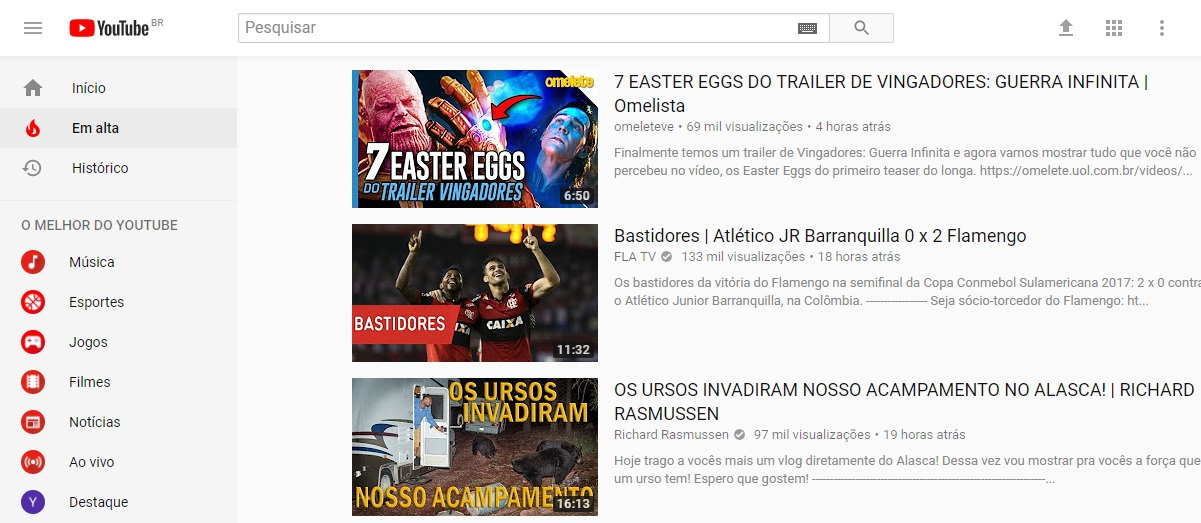
\includegraphics[scale=0.50]{imagens/youtube.jpg}
	\caption{Exemplo de lista de vídeos em alta no YouTube (2017)}
	\label{fig:youtube_em_alta}
\end{figure} 

Para construir o ranque os SRs tentam predizer qual é o item mais adequado àquele usuário \citep{Ricci2011}. Para realizar a tarefa o SR coleta dos usuários suas preferências que podem ser informadas de forma explícita, como avaliação de produtos, ou implícita interpretando suas ações como o histórico de navegação. O princípio do SR é da dependência existente entre o usuário e sua atividade em torno dos itens \citep{Aggarwal:Intro:2016}. Como exemplo, se um usuário comprou um filme de ficção científica, é mais provável que também tenha interesse em outro filme de ficção científica. Dessa forma, o sistema lida com o problema da sobrecarga filtrando itens que sejam menos prováveis do usuário gostar, baseando-se nas demonstrações do interesse prévio em outros itens, seja por outros usuários ou não.

O aumento da importância da Web como meio eletrônico, especialmente para o e-commerce, também se mostrou como força para o desenvolvimento de sistemas de recomendação.  Na Web o usuário pode facilmente informar o seu feedback de produtos sobre o que gostou ou não. Nesse contexto, a aplicação do SR não somente beneficia o usuário, mas também para aqueles que o provem \citep{ ISINKAYE2015261}. Estudos \citep{Mykolas:2015a} demonstram que usuários optam por realizar compras online para poupar tempo. Contudo, com a explosão da variedade de informação disponível, em vez de agir em benefício começa a denigrir a experiência, diminuindo a experiência de uso. É bem aceito que ter escolha é bom, mas ter mais nem sempre é melhor \citep{Ricci2011}.

É importante ressaltar que por fornecer uma informação individualizada, que esteja mais alinhada com o perfil do usuário é o que diferencia os sistemas de recomendação de sistemas de recuperação de informação. Tradicionalmente o motor de buscas deve retornar tudo correspondente a um termo de pesquisa, porém cada vez mais o usuário entra no fator desses sistemas \citep{Burke:2002:HRS:586321.586352}. Sistemas como o Google\footnote{https://www.google.com}, vão além de retornar termos que batem com a consulta, mas também com a quantidade de outras páginas referentes, histórico de buscas, localização, compatibilidade com dispositivos móveis, além de introduzir informações extra a busca, com os quadros do knowledge graph\footnote{ https://www.google.com/intl/bn/insidesearch/features/search/knowledge.html}.

\section{Conceitos}
\label{sec:conceitosSistemaRecomendacao}

Sistemas de recomendação são sistemas de processamento de informação que lidam com diversos tipos de dados para construir recomendações que tentam prever a preferência do usuário \citep{Ricci2011}.  Os dados tratam-se de basicamente de itens que serão apresentados a usuários na forma de recomendações. Técnicas de recomendação variam com dependência do tipo de conhecimento que pode ser extraído de um dado \citep{Ricci2011}. Dados de avaliações possuem pouca informação, o que resulta em técnicas diferentes em relação daquelas que dependem mais da descrição de um item ou relações com as atividades do usuário. Generalizando, SRs referem-se a três tipos de objetos: itens, usuários e transações que são as relações entre usuários e itens.

\begin{itemize}
	\item{\textbf{Itens}: Objetos que são recomendados. Podem ser caracterizados pela complexidade valor ou utilidade. O valor de um item pode ser positivo se é útil para o usuário, ou negativo se não é apropriado ou foi uma decisão errada de seleção por parte do mesmo. O usuário pode ser modelado e representado de diferentes formas, variando bastante em relação do domínio operado pelo SR. Toda vez que um usuário interage com um item constrói-se um custo cognitivo, o que pode entrar na relevância na construção do sistema, mesmo se o usuário não chega a adquirir o item interagido. Alguns exemplos de itens são: livros, notícias (baixa complexidade), computadores, viagens, vagas de trabalho (alta complexidade).}

	\item{\textbf{Usuários}: Usuários de um SR, podendo ter uma variedade de objetivos e características. São explorados uma série de informações variadas para personalizar as recomendações. A informação pode ser estruturada de diversas formas de acordo com o seu tipo, e a seleção de um modelo depende das técnicas a serem utilizadas. Modelos para sistemas de filtragem colaborativa pode usar apenas listas de avaliações de itens por usuários. O modelo de usuário cria o seu perfil, ou seja, armazena suas preferências e necessidades. Usuários também podem ser descritos baseados num padrão de comportamento, como o histórico de navegação na Web sua ou localização.}

	\item{\textbf{Transações}: Genericamente refere-se a transações gravadas das interações entre usuários e o SR. Transações podem ser vistas como um histórico de registros, um log de dados que armazena importantes informações geradas das interações com o sistema. Um registro pode conter a descrição do que foi consultado para uma recomendação particular de um item.}
\end{itemize}

\section{Tarefas de um Sistema de Recomendação}
\label{sec:tarefasSistemaRecomendacao}

Sistemas de recomendação são vistos como mais do que uma ferramenta de prover sugestões de itens que o usuário possa desejar. \citep{Ricci2011} em seu artigo introduziu uma série de funções que podem ser aplicadas a SRs.

\begin{itemize}
	\item{\textbf{Aumento do número de itens vendidos}: Uma das funções mais importantes para aplicações comerciais. O objetivo é ser capaz de vender outros itens comparados àqueles que são vendidos sem qualquer tipo de recomendação. O objetivo é geralmente alcançado devido a itens que são prováveis de serem úteis a necessidade do usuário.}

	\item{\textbf{Vender itens mais diversos}: Também outra função de alta importância, na qual permite o usuário a selecionar itens que podem ser difíceis de encontrar. Num serviço de recomendações de filmes, como o Netflix\footnote{https://www.netflix.com}, o provedor estará interessado que os usuários encontrem conteúdos diversos, não somente os mais populares.}

	\item{\textbf{Aumentar a satisfação do usuário}: Quando um usuário encontra recomendações que sejam de seu interesse, impacta na experiência com o sistema. Um SR bem desenvolvido permite uma combinação precisa de recomendações que juntos a uma interface com boa operabilidade, pode aumentar a noção subjetiva da avaliação de um sistema.}

	\item{\textbf{Aumentar a fidelidade}: Um usuário costuma ser leal a um site que, quando visitado, o reconhece como um consumidor reincidente e o trata como um visitante de valor. É muito comum para um SR levar em consideração as informações obtidas em prévias interações com o usuário. Consequentemente, por quanto mais tempo o usuário interage com o site, mais refinado seu modelo torna, tornando cada vez mais efetivo e customizado o resultado da recomendação.}

	\item{\textbf{Melhor entendimento do que o usuário quer}: Outra função importante, na qual pode ser influenciada por outras aplicações, é a descrição das preferências do usuário, seja coletada de forma explícita ou prevista pelo sistema. Um serviço pode decidir reutilizar esses dados do usuário para anunciar um produto em específico, derivado da coleta das informações de transações do SR.}
\end{itemize}

Usuários também podem desejar um SR quando oferecer suporte a suas tarefas ou objetivos. \cite{Herlocker:2004:ECF:963770.963772} é uma clássica referência no assunto, e define onze tarefas comuns que SR podem ajudar a implementar. 

\begin{itemize}
	\item{\textbf{Encontrar bons itens}: Recomendar a usuários alguns itens em ranque, junto a uma predição de o quão o usuário possa gostar deles. Também comum no uso em sistema comerciais.}

	\item{\textbf{Encontrar todo os bons itens}: Recomendar todos os itens que satisfazem as preferências do usuário. Neste caso é insuficiente apenas encontrar alguns bons itens. Esta função torna-se útil quando existe um número reduzido de itens, ou quando há uma razão crítica para fornecer informação, como em contextos de uso médico ou financeiro.}

	\item{\textbf{Anotações em contexto}: Dado um contexto, enfatizar alguns itens de uma lista a depender das preferências do usuário.}

	\item{\textbf{Recomendar uma sequência}: Recomendar uma sequência de itens invés de gerar uma única recomendação.}

	\item{\textbf{Recomendar um grupo}: Sugerir grupos de itens bem relacionados que possam ser da preferência do usuário.}

	\item{\textbf{Apenas navegando}: Mesmo que o usuário não possua a intenção de comprar um item, o SR deverá ajudá-lo a navegar pelos catálogo de maneira que encaixe no escopo de interesse do usuário.}

	\item{\textbf{Encontrar um sistema de recomendação confiável}: Nem todos os usuários podem confiar no sistema, dessa forma é importante oferecer testes de suas funcionalidades.}

	\item{\textbf{Melhorar o perfil}: Relativo a capacidade de o usuário prover dados ao SR sobre suas preferências. Tarefa fundamental para personalizar o sistema, caso contrário apenas seria possível oferecer recomendações que fosse relativa ao usuário comum.}

	\item{\textbf{Expressar-se}: Usuários podem não se importar com as recomendações, mas o sistema pode permiti-lo a contribuir com as avaliações e expressão de suas opiniões.}

	\item{\textbf{Ajudar outros}: Para alguns é importante contribuir com informações de suas opiniões e avaliações, pois compartilhando sua experiência pode ajudar outros formarem uma opinião.}

	\item{\textbf{Influenciar outros}: Alguns usuários podem ter apenas o objetivo de influenciar outros, ou até usar o SR para denegrir a imagem de alguns itens.}
\end{itemize}

\section{Técnicas de Recomendação}
\label{sec:tecnicnasRecomendacao}

As recomendações utilizadas no sistema são alcançadas através de algumas técnicas que possuem o objetivo de prever informações sobre itens e preferências de usuários. O SR irá produzir recomendações individualizadas como saída, ou será capaz de guiar o indivíduo de forma personalizada a modo de encontrar itens úteis \citep{Burke:2002:HRS:586321.586352}. Apresentadas não somente como técnicas de filtragem colaborativa, \cite{Resnick:1997:RS:245108.245121}, introduz o termo mais genérico de sistema de recomendação, uma vez que tais sistemas podem explicitamente não utilizar recipientes que talvez sejam desconhecidos uns aos outros. 

Para alcançar as principais funções de um SR, é necessário que o sistema seja capaz de identificar que itens possuem alguma utilidade para o usuário \citep{Ricci2011}. O sistema deve prever ou comparar a utilidade de itens, para decidir como recomendá-los. Dessa forma, as recomendações podem variar conforme os dados conhecidos de usuários e itens, podendo ter maior ou menor influência em uma função específica. Como exemplo, durante a etapa da predição pode ser considerado uma informação que não seja necessariamente personalizada, como apenas recomendar itens mais populares. De posse de poucas informações, ou não conclusivas, a premissa é basear-se num item que tem boa aceitação, ou seja, que é útil para muitos, com uma recomendação provável ao usuário genérico.

Ampliando ao já apresentado Tapestry \citep{Goldberg:1992:UCF:138859.138867}, nem todas as técnicas precisam ser baseadas nas informações de preferências de outros usuários. Na literatura já foram discutidos diversas técnicas, como as apresentadas nos trabalhos de \citep{Ricci2011} e  \citep{ Burke:2002:HRS:586321.586352}. Dentre essas abordagens estão:

\begin{itemize}
	\item{\textbf{Filtragem Colaborativa}: O sistema agrega avaliações ou recomendações, reconhecendo características comuns entre usuários baseando-se nos itens de suas avaliações.}

	\item{\textbf{Baseada em conteúdo}: Objetos de interesse são definidos pela associação de suas características. O sistema aprende e recomenda itens similares ao que usuário demonstrou interesse no passado.}

	\item{\textbf{Demográfico}: Objetivam categorizar o usuário baseado nas informações pessoais dos usuários. Recomendações são baseadas nas classes demográficas dos usuários.}

	\item{\textbf{Baseada em conhecimento}: Realizam sugestões de itens baseadas em inferências das preferências do usuário.}
\end{itemize}

Abaixo será apresentado em maiores detalhes o funcionamento das técnicas de filtragem colaborativa e baseada em conteúdo.

\subsection{Filtragem Colaborativa}

Recomendação com \ac{CF} é uma das técnicas mais familiares e já implementadas \citep{Ricci2011}. A similaridade das preferências e desejos de dois usuários é calculada baseada na similaridade do histórico de avaliações dos usuários. A premissa do método é de que a opinião de outros usuários pode ser selecionada e agregada de forma a prover predições razoáveis ao usuário alvo \citep{HCI-009}. Como exemplo, intuitivamente assume-se que usuários que concordam sobre a qualidade de um filme que João gosta, então João provavelmente gostará de outros filmes que outros usuários avaliaram, mas não assistiu.

O perfil de um usuário na CF pode ser continuamente aprimorado conforme o usuário interage com sistema, podendo levar o tempo de uso como fator de avaliação. Em alguns casos a avaliação pode ser apenas binária (\textit{like} ou \textit{deslike}), ou então de valor real que determina um grau de utilidade. Nesse caso, nas avaliações do usuário, o sistema deverá modelar uma função $R(u,i)$ representado o grau de utilidade do item \textit{i} para o usuário \textit{u}.  Basicamente, a tarefa do sistema é estimar um valor de \textit{R} baseado nos pares de usuário e item. Dessa forma, avaliando os dados dessas predições de \textit{R} para o usuário alvo, o sistema recomendará uma quantidade de itens com as maiores utilidades previstas.

Tipicamente, conforme apresentado por \cite{Burke:2002:HRS:586321.586352}, CF divide-se em dois método principais: vizinhança e baseados em modelo. No método da vizinhança o foco é no relacionamento entre itens ou usuários, conhecidos como de \textit{item-item} ou \textit{usuário-usuário} \citep{Ricci2011}, utilizando informações armazenadas com o tempo. O método aborda modelos através da análise da preferência armazenada das classificações de usuário-item, pela avaliação de outros itens similares. Já o método baseado em modelo é criado diretamente do histórico das avaliações para aprender as preferências do usuário, podendo-se usar uma quantidade diversa de técnicas para o aprendizado, como redes neurais. O objetivo é compreender e extrair das interações usuário-item características de destaque para o sistema, podendo criar classes de preferências dos itens.

\subsection{Filtragem Baseada em Conteúdo}

Ao contrário da filtragem colaborativa, sistemas de recomendação baseados em \ac{CBF}, seleciona itens baseados entre as relações de seus conteúdos e as preferências do usuário. A CBF é uma continuação natural das pesquisas nos sistemas de filtragem de informação, \cite{Burke:2002:HRS:586321.586352}.  O método utiliza-se da intuição de que se o usuário demonstrou interesse em certos itens com determinados atributos, é provável de também ter interesse em outros itens de mesmo atributo ou semelhante. Como exemplo, se João gostou dos filmes com o ator \textit{Tom Cruise}, é provável que vá gostar de outros filmes com o mesmo ator. Os sistemas de CBF foram desenhados para explorar cenários com itens que podem ser descritos com um conjunto de propriedades ou atributos \citep{Aggarwal2016}.

Nessa abordagem, o sistema deverá aprender do perfil do usuário seus interesses baseados na combinação das características presentes nos objetos que ele avaliou ou marcou.  O tipo do perfil utilizado no sistema dependerá do método aplicado. A informação das preferências do usuário pode manifestar-se de forma explícita, onde existem avaliações ou indicações dos itens favoritos, ou de forma implícita como itens que o usuário comprou. Nos métodos aplicados na CBF, as descrições dos itens avaliados são usadas como dados de treinamento para criar uma classificação específica para o usuário \citep{Aggarwal2016}. Os perfis da filtragem baseada no conteúdo são modelos de longo prazo, onde mais dados são atualizados conforme mais evidências do usuário são observadas, \cite{Burke:2002:HRS:586321.586352}.

Apesar da descrição do conteúdo, ou seja, atributos particulares dos itens, sejam o centro da análise da utilidade de novos itens para recomendação, a avaliação de outros usuários tem significativo impacto no sistema \citep{Aggarwal2016}. Essa característica apresenta tanto vantagens como desvantagens. Por um lado, num contexto da \textit{partida a frio}, onde há pouca informação disponível sobre as avaliações dos usuários, há margem de utilização enquanto houver outras suficientes informações das preferências do usuário. Mesmo quando um item é novo ou desconhecido, o sistema ainda pode aproveitar suas características para recomendar novos itens, algo que não é possível apenas baseando-se nas avaliações de outros usuários. 

Assim, sistemas de CBF são tipicamente utilizados quando há suficiente informação das preferências do usuário disponíveis. Particularmente, são de mais fácil utilização quando usados em domínios com dados não estruturados e ricos em textos, como páginas da Web.

%\subsection{Arquitetura de Sistemas de Recomendação Baseados em Conteúdo}
	
\subsection{Comparação das Técnicas de Recomendação}

Todas as abordagens dos SR possuem vantagens e desvantagens, dependendo de questões como novos itens, usuários, e quantidade de informação disponível sobre os dois. Em relação a novos usuários, como recomendações partem da comparação de informações do usuário alvo e outros usuários, quanto menos avaliações o sistema possuir, mais difícil será a classificação. Já para novos itens, o problema surge em domínios em constante atualização e novas informações e onde cada usuário pouco avalia. Também pode ser visto como o problema do \textit{early rater}, uma vez que a pessoa que avalia primeiro, pouco se beneficia.

\cite{Burke:2002:HRS:586321.586352} apresentou alguns pontos comuns das diferenças desses sistemas:

\begin{itemize}
	\item{\textbf{Sistemas baseados em filtragem colaborativa}: Dependem da sobreposição de avaliações através dos usuários e possuem dificuldades quando há escassez dessas avaliações dos itens. O problema ressalta que as técnicas colaborativas melhor servem quando a densidade de interesses de usuários é alta através de um universo de itens que não mudam rapidamente.} 

	\item{\textbf{Sistemas baseados em conteúdo}: Possuem o problema da partida a frio, onde o sistema não acumulou dados suficientes para construir uma recomendação confiável. Também são limitados pela quantidade de informações disponíveis e associadas aos itens. Isto acaba colocando a técnica muito dependente da descrição dos dados. Uma grande desvantagem em relação a abordagem colaborativa é que a abrangência de gêneros, onde deixa o usuário sujeito ao mesmo tipo de conteúdo. A depender da CF, pela a avaliação de outros usuários é possível recomendar itens “fora da caixa”.}
\end{itemize}

\section{Aplicações de Sistemas de Recomendação}

O sistema Tapestry \citep{Goldberg:1992:UCF:138859.138867} foi um marco inicial no desenvolvimento de aplicações, introduzindo a filtragem colaborativa. Hoje, SR são quase que obrigatórios para muitas lojas online e serviços de entretenimento, tornou-se algo comum e já disseminado entre usuários. A seguir será apresentado algumas aplicações em destaque que usam sistemas de recomendação.

\subsection{Netflix}

Com a evolução da Internet, as mídias físicas para consumo de entretenimento começaram a decair, especialmente para filmes. O avanço na conexão da banda larga trouxe o modelo do \textit{streaming}\footnote{Transmissão contínua de mídia pela Internet, (https://directradios.com/streaming)} que possibilita o usuário a assistir o conteúdo a qualquer momento, lugar, sem ter que  necessariamente sair de sua residência para ir à uma locadora, por exemplo. Embora o Netflix\footnote{https://www.netflix.com}, tenha iniciado no ramo de aluguel de \ac{DVD}s \citep{keating2012netflixed}, a companhia rapidamente abandonou este modelo e partiu para a transmissão de filmes e em seguida para produção de seus próprios filmes e séries. Dessa forma, o serviço de filmes e séries cresceu, ocupou espaço das televisões, cinemas e alcançou diversos países.

\begin{figure}
	\centering
	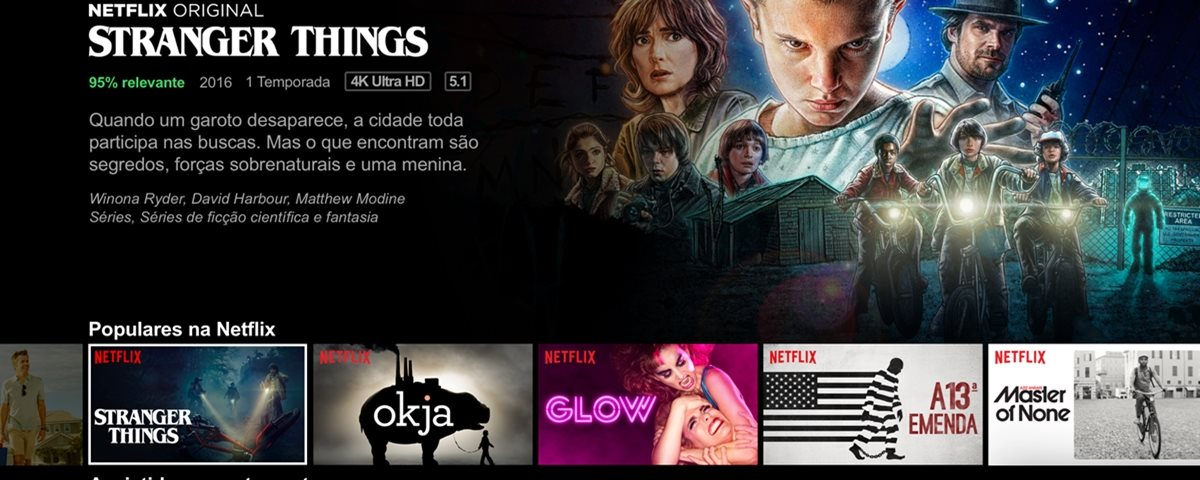
\includegraphics[scale=0.40]{imagens/netflix_recsys.jpg}
	\caption{Recomendação de Filmes no serviço Netflix. Figura elaborada pelo autor (2017).}
	\label{fig:netflix}
\end{figure}

Com a crescente quantidade de títulos disponíveis na plataforma e também de usuários, logo o serviço desenvolveu seu próprio sistema de recomendações de vídeos, baseado nas avaliações de usuários. Em outubro de 2006 a companhia publicou um concurso pelo melhor sistema de filtragem colaborativa que poderia superar a precisão de seu SR, o Cinematch \citep{bennett2007netflix}. Neste ponto o serviço já tinha lançado um banco de dados contendo 100 milhões de avaliações de usuários e 18 mil títulos. O Cinematch analisava as avaliações acumuladas dos usuários semanalmente usando uma variante da correlação de Pearson, com todos os outros filmes para determinar uma lista de filmes similares. Sendo assim, conforme o usuário provia avaliações, o sistema computava uma regressão baseada nessa correlação para determinar uma predição única personalizada. Caso não houvesse nenhuma predição personalizada a média de todas as avaliações é usada. As predições eram apresentadas como conjunto de 5 estrelas.

O desempenho do Cinematch é medido principalmente pelo cálculo da raiz do erro quadrático médio, \ac{RMSE} \citep{Herlocker:2004:ECF:963770.963772}, das predições do sistema contra as avaliações que os usuários informam. Com os sistemas propostos no concurso, a companhia propôs um prêmio para aqueles que conseguissem melhorar a precisão em 10\%. Nesse ano de 2017, a companhia migrou seu sistema de avaliação das tradicionais 5 estrelas para uma avaliação binária, o \textit{Like} e \textit{Dislike} \citep{ VarietyNetflix:2017}. Segundo a companhia, os usuários confundiam a avaliação de 5 estrelas, pois na verdade eram sempre as predições avaliadas para o filme, assim agora as predições aparecem no formato de porcentagem de relevância e a avaliação do usuário é indicada pelos símbolos do gostei ou não gostei. As predições também passaram a serem baseadas apenas no histórico e comportamento do usuário e não mais na média em relação às outras pessoas.

\subsection{Skoob}

Em janeiro de 2009, o analista de sistemas Lindeberg Moreira realizou sua ideia de criar uma plataforma em que pessoas socializassem o ato da leitura \citep{SkoobSocializando:2009}, o Skoob\footnote{ https://www.skoob.com.br}. O sistema criado trata-se de uma rede social para leitores no Brasil \citep{SkoobQuemSomos:2017}. Na plataforma, o usuário montará uma estante virtual realizando buscas pelos livros e em seguida indicar o que já fez com o livro, se já leu, se lerá ou está relendo. Após a seleção dos livros os usuários poderão avaliar seus livros, podendo até escrever resenhas completas ou de capítulos dos livros, compartilhando com outras pessoas na plataforma.

\begin{figure}
	\centering
	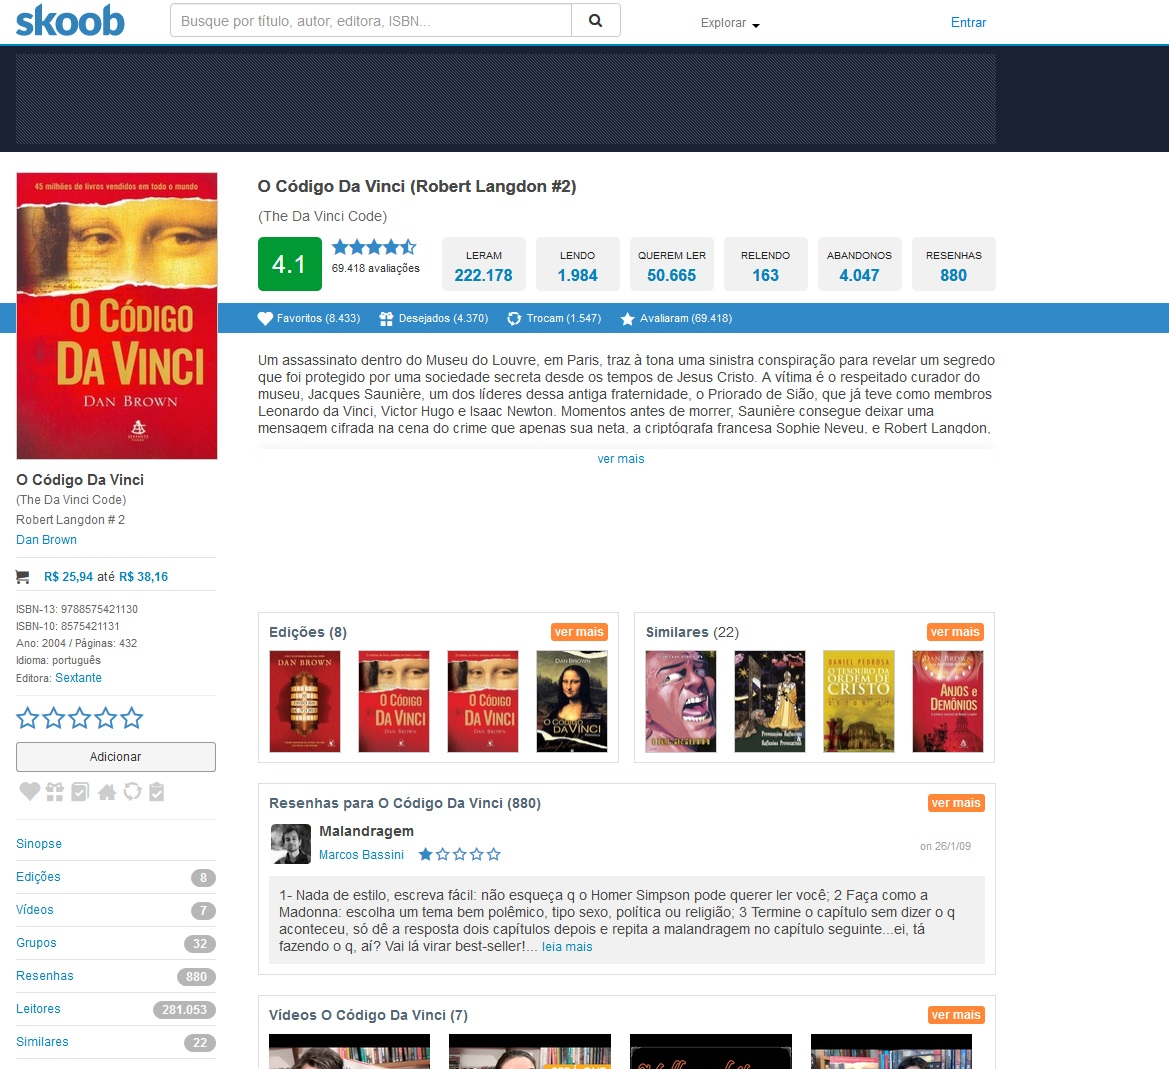
\includegraphics[scale=0.40]{imagens/skoob_recsys.jpg}
	\caption{Página de avaliação do livro no Skoob. Figura elaborada pelo autor (2017).}
	\label{fig:skoob}
\end{figure}

A rede social, conta com algumas mecânicas para ajudar usuários a encontrar livros, com um sistema busca de livros, recomendação com filtragem colaborativa baseada nas avaliações de usuários, dos marcados como mais lidos, lendo, quero ler entre outros. A plataforma também conta com um sistema que indica livros similares. Todos esses processos não somente levam a questão da socialização da leitura e escrita entre indivíduos que compartilham interesses, surgidas a partir da aplicação, mas passam a influenciar a forma como usuários passam a tratar a leitura fora do ambiente da comunidade virtual, é o que aponta \cite{SkoobUFPE:2010}.

\section{Sumário}

Neste capítulo, foi apresentado um panorama geral sobre os sistemas de recomendação. Inicialmente abordando o histórico envolvido e motivações na criação dos conceitos envolvidos do tema. Em sequência foi aprofundado e explicado os conceitos utilizados nesses sistemas. Então, foi apresentado as tarefas e técnicas utilizadas. Também foi aprofundado algumas diferenças e dificuldades entre as principais técnicas de recomendação. Por fim, foi mostrado exemplos de aplicações que utilizam esses sistemas de recomendação. No capítulo \ref{cap:semantic_web} será discutido sobre os conceitos envolvidos na Web Semântica, bem como os princípio dos dados ligados e o serviço da DBPedia\footnote{http://wiki.dbpedia.org}.
\chapter{Web Semântica}
\label{cap:semantic_web}

\begin{quotation}[]{Tim Berners-Lee}
I found myself answering the same questions asked frequently of me by different people. It would be so much easier if everyone could just read my database
\end{quotation}

A introdução e expansão da \textit{World Wide Web} possibilitou acessar e publicar uma grande variedade de conteúdo, seja para o consumo de entretenimento, exposição de opiniões, compras online etc. O crescimento da rede tornou-se tão grande que é latente a dificuldade dos usuários encontrar informações. Para eles, foram criados e desenvolvidos os indexadores de páginas, como o Google\footnote{https://www.google.com}, Yahoo\footnote{https://www.yahoo.com}, Bing\footnote{https://www.bing.com}. Tais sistemas facilitam encontrar informações em serviços populares na Internet. Entretanto, e se quiséssemos encontrar algum médico de confiança para marcar uma consulta, levando em consideração uma agenda de compromissos? Ou então se estamos realizando um trabalho escolar e queremos encontrar os reis do século XV? Essas pesquisas certamente são mais complicadas, e resultados de buscas tradicionais levam a informações fragmentadas, com uma série de outras buscas separadas para alinhar todo o conhecimento e semântica envolvidos nessas tarefas. É nesse ponto que entra o conceito da Web Semântica, como uma extensão da já existente.

O conteúdo da Web tradicional é fundamentalmente desenvolvido para humanos lerem, não para máquinas manipularem de forma produtiva e significante \citep{bernerslee2001semantic}. Originalmente desenvolvida para compartilhar e apresentar conteúdo de forma que fosse possível interagir e navegar entre hipertextos e hipermídia, a \ac{WWW} torna fácil a apresentação de layouts. É possível estruturar um documento com um cabeçalho, um link para outra página, entretanto, dificilmente as máquinas poderão processar semanticamente que informações estão disponíveis e que podem ser organizadas naquela página ou site. Como exemplo, uma página de João com link para seu currículo informando que possui especialização em cardiologia. Todas essas informações podem até serem compreendidas por humanos ao associar a semântica das entidades presentes numa página e analisando links relacionados, mas para a máquina não há uma estrutura comum e eficiente que leve a essas mesmas conclusões.

O objetivo da Web Semântica é de estender a WWW, aproveitando a enorme variedade de dados já existente, mas agregando uma nova camada de metadados que possibilitem o processamento pela máquina e agentes de forma a compreender a semântica das informações apresentadas. Assim, a Web Semântica trata-se de prover formatos para integração de dados de diferentes fontes \citep{SemanticWebW3C}, onde a Web tradicional mantém-se como o meio de publicação e interconexão de documentos, e na contraparte semântica, armazena-se dados que se relacionam com objetos e coisas do mundo real. Um agente pode se deparar com uma página de clínica na Web e não apenas compreenderá que possui palavras como “tratamento, terapia, remédios, médicos”, como tipicamente é encontrado na Web tradicional, mas também saber que o "Dr João" trabalha nessa clínica nas segundas e quartas com horários no formato \textit{dd/mm/YYYY}.

\section{Arquitetura e formato de dados}

O funcionamento da Web Semântica depende da capacidade de máquinas acessar coleções estruturadas de informações, dados e regras de inferência para executar raciocínio automatizado \citep{bernerslee2001semantic}. O desafio é de como representar conhecimento. Inicialmente o desenvolvimento desses sistemas utilizaram uma abordagem centralizadora, requerendo que as partes envolvidas compartilhem exatamente as mesmas definições de conceitos comuns ou hierárquicos. Entretanto, com a quantidade de conteúdo existente hoje em diferentes línguas, controle centralizado é desafiador. Contrastando essa visão inicial, na Web Semântica cria-se linguagens para regras as quais são tão expressivas quanto o necessário para que a Web seja ampla como desejado \citep{bernerslee2001semantic}. Com um sistema que não seja centralizado é possível que não se responda todas as perguntas, ou seja, encontrado todas as informações, mas permite que regras sejam usadas para criar inferências e escolher o curso de ações para poder ou tentar responder tais perguntas.

Com esses fundamentos os pesquisadores da Web Semântica, em especial o \textit{World Wide Web Consortium}, desenvolveram uma série de padrões e formatos de dados para o uso na Web. O intuito é possibilitar máquinas compreenderem documentos com dados semânticos e não discursos e textos criados pelo homem. Uma tecnologia muito importante para o desenvolvimento da representação do conhecimento e protocolo de comunicação entre máquinas, foi a \ac{XML}. Com a XML é possível que qualquer um seja capaz de criar suas próprias \textit{tags} e estruturas de um documento com definição de cada termo presente de forma arbitrária. Desse ponto de vista a XML é fundamental como um padrão de comunicação entre máquinas. Anos seguintes, a W3C introduziu outras três importantes tecnologias presentes no cenário atual da Web Semântica: \ac{RDF}, \ac{SPARQL}, \ac{OWL}.

\subsection{RDF}

Resource Descripton Framework é um modelo de dado para a Web que facilita a junção de dados mesmo que seu \textit{schema} difira, além de permitir a sua evolução sem requerer que seus consumidores tenham que se adaptar \citep{W3CRDF}. No RDF a estrutura da \textit{web} de links é estendida para usar os \ac{URI} para nomear a relação entre qualquer coisa, com ambas as pontas, formando o que é conhecido como a tripla.

\begin{figure}
	\centering
	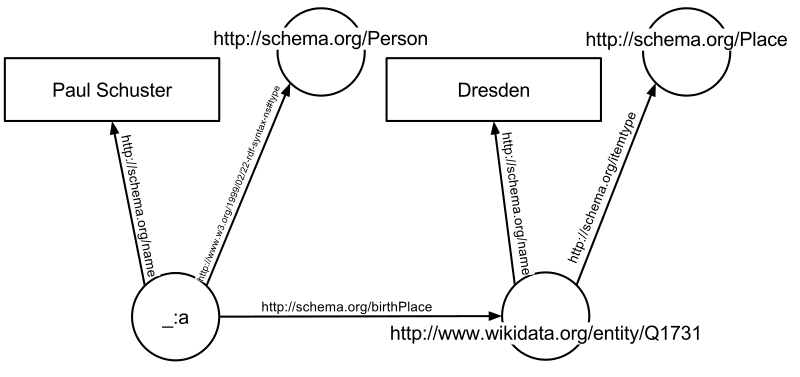
\includegraphics[scale=0.40]{imagens/rdf_example1.png}
	\caption{Exemplo do grafo RDF \citep{RDFWikiImage}}
	\label{fig:rdf_graph}
\end{figure}

\begin{figure}
	\centering
	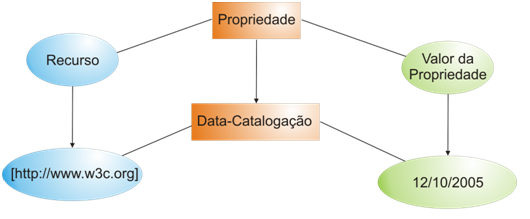
\includegraphics[scale=0.65]{imagens/rdf_example2.png}
	\caption{Exemplo do grafo da tripla sujeito predicado objeto \citep{WebSemanticaDevmedia}}
	\label{fig:rdf_graph2}
\end{figure}

O uso da URI é especialmente notável para a Web, uma vez que não é possível apenas se basear em valores literais, mesmo para representar um atributo de algo, já que é desejado ter a definição e estrutura podendo considerar um domínio em específico. Como exemplo, com uma URI é possível identificar de forma única o predicado “título” que se refere ao título da função em uma empresa, e não um título de filme. Então, a tripla forma um grupo de três entidades que expressam uma declaração sobre o dado semântico, na forma de “sujeito, predicado, objeto”. Com essa estrutura de links é formado um grafo direcionado, com \textit{labels}, aonde suas arestas representam o link nomeado entre dois recursos representados pelos seus nós \citep{W3CRDF}.

\subsection{SPARQL}

O SPARQL é uma linguagem de consulta para o grafo do RDF \citep{SparqlW3C}. Dessa forma, pode-se criar \textit{queries} através de diversos conjuntos de dados de triplas, podendo ser aplicado uma série de filtros para limitar e ordenar os resultados retornados. Diferentemente das linguagens de consulta de banco de dados relacionais, o objeto da coluna não é homogêneo, ou seja, o tipo dado da célula da tabela de resultados é implicado ou definido pelo predicado informado através da URI. O sujeito do RDF pode ser classificado com um análogo a uma entidade nos bancos de \ac{SQL}, diferindo onde os campos (ou atributos) são representados como predicados e/ou objetos separados.

O exemplo do Código Fonte \ref{cod:sparql-example} demonstra a consulta de dados de uma ontologia \textit{foaf}\footnote{http://xmlns.com/foaf/spec/}, conhecida como "friend of a friend".

\begin{lstlisting}[caption=Exemplo de consulta na linguagem SPARQL, language=SPARQL, frame=single, label={cod:sparql-example}, float, numbers=left]
PREFIX foaf: <http://xmlns.com/foaf/0.1/>
PREFIX rdf: <http://www.w3.org/1999/02/22-rdf-syntax-ns#>
SELECT ?name
       ?email
WHERE
  {
    ?person  a          foaf:Person .
    ?person  foaf:name  ?name .
    ?person  foaf:mbox  ?email .
  }
}
\end{lstlisting}

\subsection{OWL}

Ontology Web Language é uma linguagem para definir e instanciar ontologias na Web \citep{OWLW3C}. Um programa que deseja comparar ou combinar informações entre dois bancos de dados com URIs distintas, deve saber se termos podem ser usados para descrever o significado da mesma coisa \citep{bernerslee2001semantic}. O objetivo é que um programa descubra o significado comum seja para o que for encontrado entre os conjuntos de dados. A solução proposta na Web Semântica para esse problema é a utilização de uma coleção de informações denominadas de ontologias. Na filosofia uma ontologia tem por objeto o estudo das propriedades do ser, tratando da natureza da existência. Entretanto, no campo da inteligência artificial e na Web, é definido como os termos básicos e relações que compreendem um vocabulário de um domínio, bem como regras para combiná-los junto com relações para definir extensões desse vocabulário \citep{Patil:1992:DKS:3087223.3087302}.

Em essência a ontologia é um documento que define formalmente as relações entre termos. As ontologias podem ser vistas de forma semelhante à hierarquia de classes na programação orientada a objetos. Tipicamente uma ontologia para a Web possui uma taxonomia e um conjunto de regras de inferência. A taxonomia define classes (ou conceitos) de objetos e suas relações, sendo assim, um endereço pode ser definido como um tipo de localidade e o código de uma cidade pode ser definido para ser aplicado apenas a localizações, entre outros exemplos.

A linguagem OWL provê três sublinguagens, OWL Lite, OWL DL, OWL Full como apresentado pela \cite{OWLW3C}.

\begin{itemize}
	\item{\textbf{OWL Lite}: Para a criação hierárquica e simples de limitações de \textit{features}. Como exemplo, é possível oferecer suporte a limitações de cardinalidade que só permitam valores de 0 ou 1. É mais simples de prover suporte.}

	\item{\textbf{OWL DL (descrição lógica)}: Oferece suporte a uma expressividade máxima sem perder a completude computacional (todas as implicações são garantidas para serem computadas), decidibilidade (todos os cálculos finalizaram em um tempo finito). Inclui todas as construções com restrições e separação de tipos (uma classe também não pode ser indivíduo ou propriedade, uma propriedade também não pode ser um indivíduo ou uma classe).}

	\item{\textbf{OWL Full}: Oferece o máximo de expressividade e é sintaticamente livre do RDF sem garantias computacionais. Nessa linguagem uma classe pode ser tratada simultaneamente como uma coleção de indivíduos ou indivíduo como todo. Então, a OWL Full permite uma ontologia ter seu significado ampliado ao pré-definido (RDF ou OWL) vocabulário.}
\end{itemize}

Todas as sub-linguagens são extensões de sua predecessora, sendo assim cada ontologia válida em OWL Lite é uma ontologia válida em OWL DL que por sua vez é uma ontologia válida em OWL Full \citep{OWLW3C}. É notável destacar que o inverso das relações não é verdadeiro. Completando, todo documento OWL é um documento em XML construído com o RDF.

\subsubsection{Estrutura de um documento}

Com a OWL é possível descrever de forma natural classes e relacionamentos entre documentos e aplicações na Web \citep{OWLReport:2005}. Os termos descritos devem estar dispostos de tal maneira que não cause ambiguidade, assim é necessário que seja informado quais vocabulários serão empregados. Para o uso de vocabulários a \cite{OWLW3C} informa que deve-se definir no topo do documento os \textit{xml namespaces} \footnote{No XML, os namespaces são nomes únicos para elementos e atributos no documento. Para resolver as ambiguidades e facilitar as referências antes dos nomes são utilizados prefixos}, conforme mostrado no código fonte \ref{cod:owl-prefixes}.

\begin{lstlisting}[caption=Exemplo do topo de um documento OWL, language=XML, frame=single, label={cod:owl-prefixes}, float, numbers=left]
<rdf:RDF
    xmlns     ="http://www.w3.org/TR/2004/REC-owl-guide-20040210/wine#"
    xmlns:vin ="http://www.w3.org/TR/2004/REC-owl-guide-20040210/wine#"
    xml:base  ="http://www.w3.org/TR/2004/REC-owl-guide-20040210/wine#"
    xmlns:food="http://www.w3.org/TR/2004/REC-owl-guide-20040210/food#"
    xmlns:owl ="http://www.w3.org/2002/07/owl#"
    xmlns:rdf ="http://www.w3.org/1999/02/22-rdf-syntax-ns#"
    xmlns:rdfs="http://www.w3.org/2000/01/rdf-schema#"
    xmlns:xsd ="http://www.w3.org/2001/XMLSchema#">
\end{lstlisting}

Acrescentando, a \ac{W3C} recomenda incluir no documento um cabeçalho XML que preceda as definições das ontologias como apresentado no código fonte \ref{cod:owl-head}

\begin{lstlisting}[caption=Exemplo do cabeçalho XML de um documento OWL, language=XML, frame=single, label={cod:owl-head}, float, numbers=left]
<!DOCTYPE rdf:RDF [
    <!ENTITY vin  "http://www.w3.org/TR/2004/REC-owl-guide-20040210/wine#" >
    <!ENTITY food "http://www.w3.org/TR/2004/REC-owl-guide-20040210/food#" > ]>
\end{lstlisting}

\begin{lstlisting}[caption=Exemplo de propriedades transitivas no OWL, language=XML, frame=single, label={cod:owl-props}, float, numbers=left]
<owl:ObjectProperty rdf:ID="subordinate">
    <rdf:type rdf:resource="&owl;TransitiveProperty"/>
    <rdfs:domain rdf:resource="#Agent"/>
    <rdfs:range rdf:resource="#Agent"/>
</owl:ObjectProperty>

<Agent rdf:ID="Joao">
    <subordinate rdf:resource="#Pedro"/>
</Agent>

<Agent rdf:ID="Pedro">
    <subordinate rdf:resource="#Maria"/>
</Agent>
\end{lstlisting}

\begin{lstlisting}[caption=Exemplo do cabeçalho de uma ontologia, language=XML, frame=single, label={cod:owl-ontology-head}, float, numbers=left]
<owl:Ontology rdf:about="">
  <rdfs:comment>An example OWL ontology</rdfs:comment>
  <owl:priorVersion rdf:resource="http://www.w3.org/TR/2003/PR-owl-guide-20031215/wine"/>
  <owl:imports rdf:resource="http://www.w3.org/TR/2004/REC-owl-guide-20040210/food"/>
  <rdfs:label>Wine Ontology</rdfs:label>
  ...
\end{lstlisting}

Por último será informado o cabeçalho da ontologia junto a suas propriedades. Nesse cabeçalho é importante fornecer informações sobre ela própria. Para descrevê-las utiliza-se as propriedades do OWL, uma vez que a ontologia é um recurso, assim demonstrado no código fonte \ref{cod:owl-ontology-head}

Dentro da definição da ontologia poderão ser informados as classes e indivíduos relacionados como as propriedades e suas relações. As propriedades podem ser descritas como transitivas, simétricas, funcionais ou inversamente funcional. Como exemplo, numa propriedade transitiva de subordinado, se é dito que João é subordinado de Pedro e Pedro é subordinado de Maria, portanto João é subordinado de Maria. No código fonte \ref{cod:owl-props} é demonstrado a declaração desse tipo de propriedade.

\subsection{Estrutura na rede semântica}

\begin{figure}
	\centering
	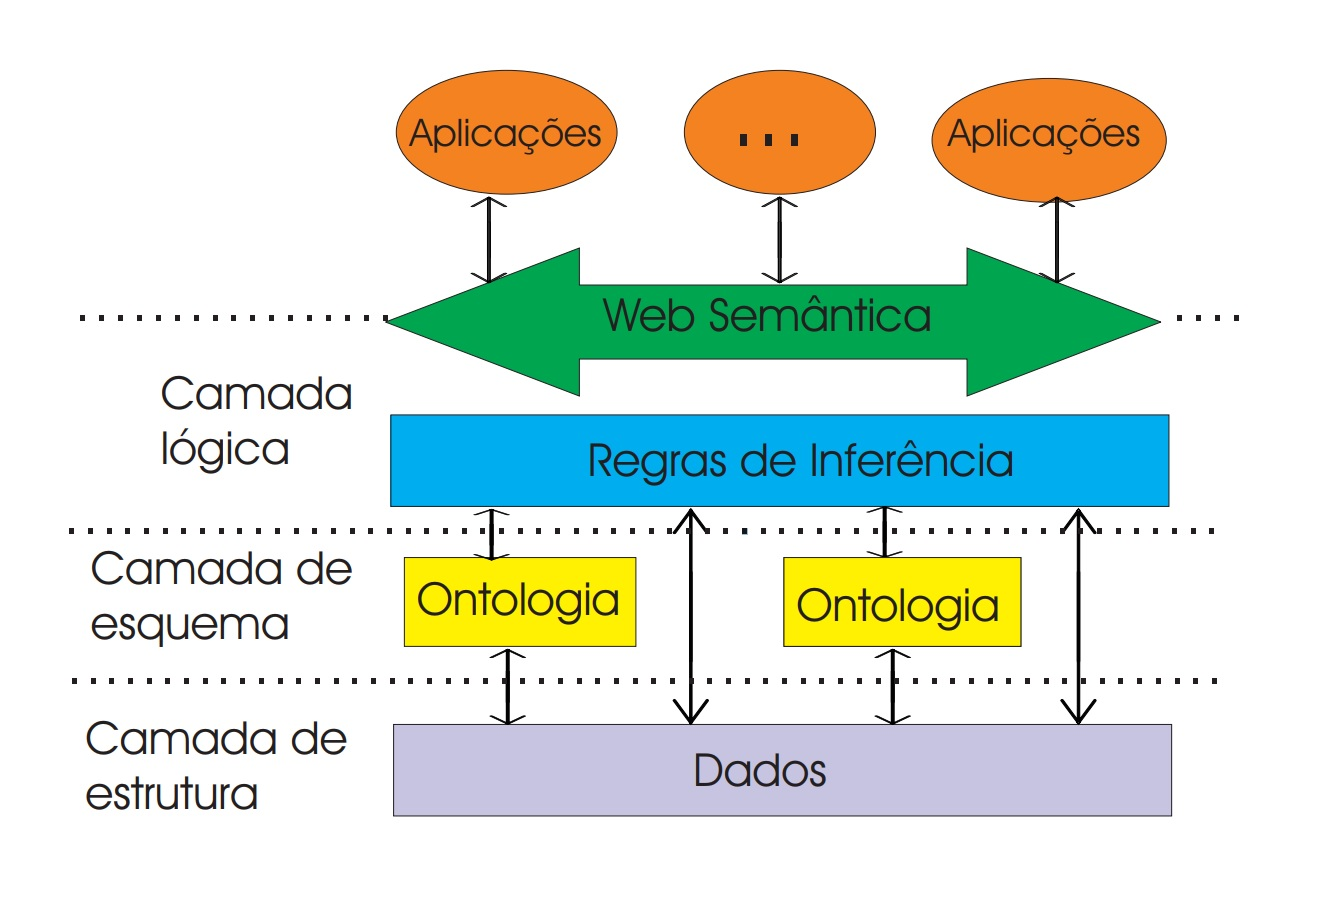
\includegraphics[scale=0.35]{imagens/sw_layers.jpg}
	\caption{Camadas na rede semântica. \citep{OWLReport:2005}}
	\label{fig:sw-layers}
\end{figure}

\begin{figure}
	\centering
	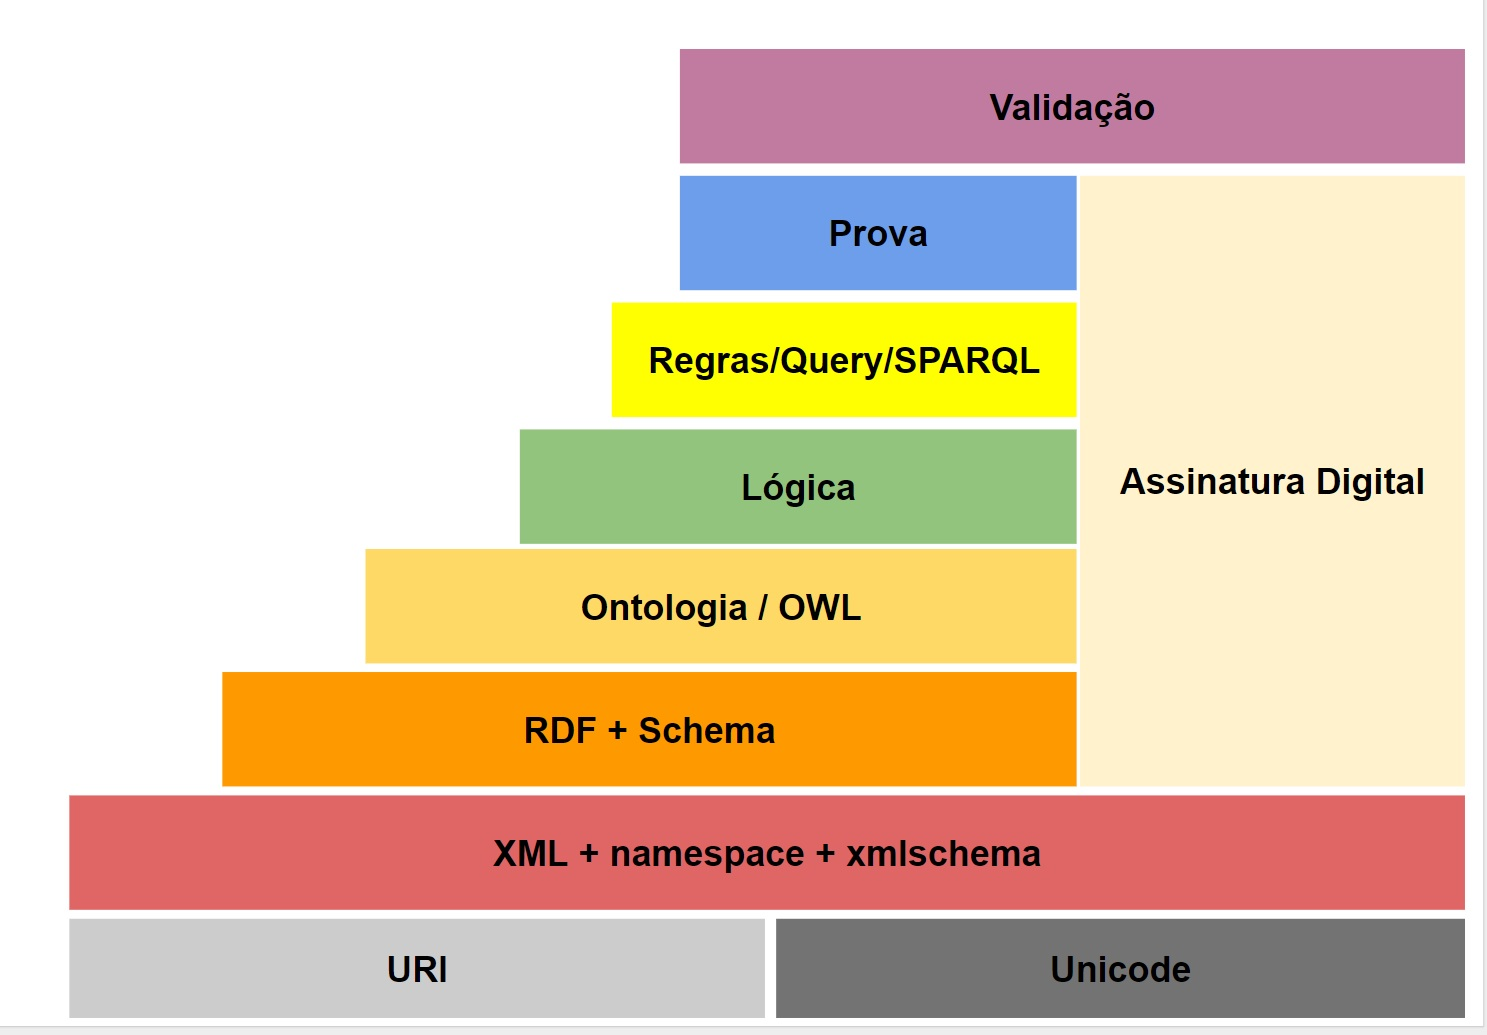
\includegraphics[scale=0.30]{imagens/sw_w3c_stack.jpg}
	\caption{Camadas na rede semântica. Figura elaborado pelo autor de acordo com a publicação de \cite{SemanticWebStack}}
	\label{fig:sw-w3c-stack}
\end{figure}

A introdução das tecnologias para alcançar os princípios idealizados na Web Semântica são implantados em camadas. De acordo com \cite{bernerslee2001semantic} é possível dividir esses serviços em três grandes camadas, como demonstrado na Figura \ref{fig:sw-layers}. Na camada de estrutura os dados são organizados e definidos seus significados, na qual utiliza-se as triplas do RDF. A camada com os esquemas estão as ontologias, utilizando-se o OWL para a representação de conceitos, inferências através das taxonomias e conjunto de regras. Por último na camada lógica é definida para fazer inferência sobre os dados. Dessa forma, o desenvolvimento dessas tecnologias (ainda em andamento) e padronização dos formatos foi formulado pela W3C como uma pilha das camadas \citep{SemanticWebStack} da Web Semântica confiável, conforme mostrado na figura \ref{fig:sw-w3c-stack}.

\section{Dados ligados}

A evolução da WWW tornou cada vez mais acessível a publicação e acesso a documentos pela navegação no espaço global, através links dos hipertextos \citep{Bizer2009}. Com os navegadores da Web pode-se passear pelos links nesse espaço e em especial com o uso dos buscadores, que indexam páginas para facilitar a recuperação. Tais mecanismos já estão amplamente difundidos na publicação de documentos, mas quando comparados aos dados\footnote{Note que embora os termos "dados" e "documentos" possam ser análogos, no contexto da Web, documentos tratam-se das páginas dos sites e dados, de fato a informação em si. Assim, na Web os documentos apenas objetivam o aspecto da apresentação não contento a semântica dos dados presentes.} em si, esses princípios ainda foram timidamente aplicados. Assim, com o crescimento da Web Semântica trouxe-se a ênfase em criar uma Web para os dados, capaz descrever entidades individuais presentes nos documentos, conectando-se por links categorizados para relacionar tais entidades. O objetivo não é somente colocar dados na Web, mas utilizar links que ambas máquinas (principalmente) e humanos possam navegar.

Suportando essa evolução da Web \citep{LinkedData:2006} introduziu um conjunto de melhores práticas para a publicação e conexão de dados estruturados na Web, denominado de \textit{Linked Data} (dados ligados). A adoção dessas práticas permite a extensão da Web como um espaço de dados global conectado de diversos domínios, desde pessoas, livros, publicações até dados governamentais dos mais variados assuntos. Com essa Web de dados surge a oportunidade para novos tipos de aplicações \citep{Bizer2009}, como navegadores customizados para um determinado domínio podendo saltar entre diferentes fontes de dados.

Resumidamente, a \cite{LinkedDataW3C} define que para a Web de dados ser uma realidade é necessário que os dados estejam disponíveis em padrões de formatos que sejam buscáveis e manipuláveis pelas ferramentas e tecnologias da Web Semântica. Complementando, é preciso também ter acesso ao relacionamento de dados. O conjunto de \textit{datasets} inter-relacionados na Web, para criar links tipificados entre dados de diferentes fontes é o que se denomina de dados ligados.

Ao contrário dos documentos \ac{HTML} na Web dos hipertextos, os dados ligados se baseiam-se nos documentos contendo dados em RDF. Assim são construídos links que são tipificados para realizar declarações sobre coisas arbitrárias no mundo. \cite{LinkedData:2006} enumerou um conjunto das regras para a publicação e conexão dos dados, conhecidos como os princípios dos dados ligados:

\begin{enumerate}
	\item{Usar URIs para nomear coisas}
	\item{Usar \ac{HTTP} URIs para que pessoas possam procurar seus nomes.}
	\item{Quando alguém procura uma URI, forneça informação útil, utilizando os padrões como RDF e SPARQL.}
	\item{Inclua links para outras URIs, para que assim eles possam descobrir mais coisas.}
\end{enumerate}

Um exemplo notável do uso das dados ligados, é o projeto da DBPedia\footnote{ http://wiki.dbpedia.org} que essencialmente torna o conteúdo da Wikipedia\footnote{https://www.wikipedia.org} disponível em RDF.

\subsection{Linked Open Data}

Posteriormente em 2010, para incentivar o uso dados ligados no meio governamental, \cite{LinkedData:2006} desenvolveu um "sistema de avaliação" dos dados ligados. O objetivo era expandir o termo introduzindo os dados abertos, onde fossem publicados sob uma licença que não impede o livre reuso. No sistema de avaliação consta um esquema de pontuação em estrelas de 1 a 5, onde cada estrela a mais também acumula as definições das estrelas anteriores, conforme consta na figura \ref{fig:lod-rating}.

O \ac{LOD} tornou-se o projeto de maior adoção dos princípios dos dados ligados \citep{Bizer2009}, sendo um esforço colaborativo iniciado em 2007 para suportar as definições e tecnologias da Web Semântica introduzidas pela W3C. O motim para o início da colaboração era de mapear os dados da Web identificando os conjuntos que já estavam disponíveis sob licença aberta. O projeto inclui dados de várias fontes, como a Wikipedia\footnote{https://www.wikipedia.org}, Geonames\footnote{http://www.geonames.org}, Wordnet\footnote{https://wordnet.princeton.edu} entre diversos outros de múltiplos domínios, alcançando um impressionante diagrama como mostrado na Figura \ref{fig:lod-graph}.

\begin{figure}
	\centering
	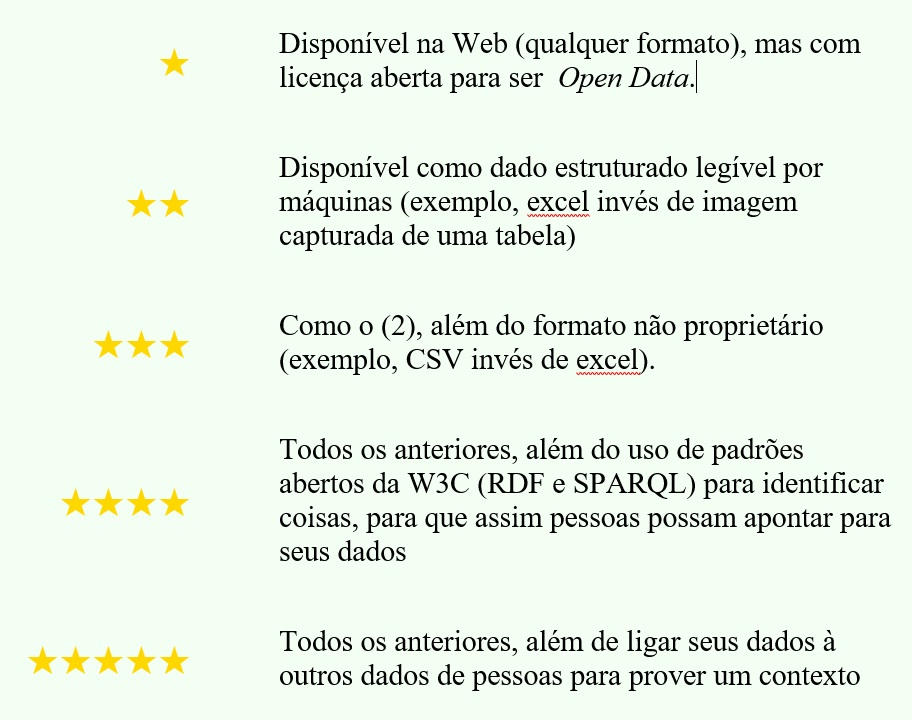
\includegraphics[scale=0.50]{imagens/lod_rating.jpg}
	\caption{Sistema de avaliação do LOD \citep{SemanticWebStack}}
	\label{fig:lod-rating}
\end{figure}

\begin{figure}
	\centering
	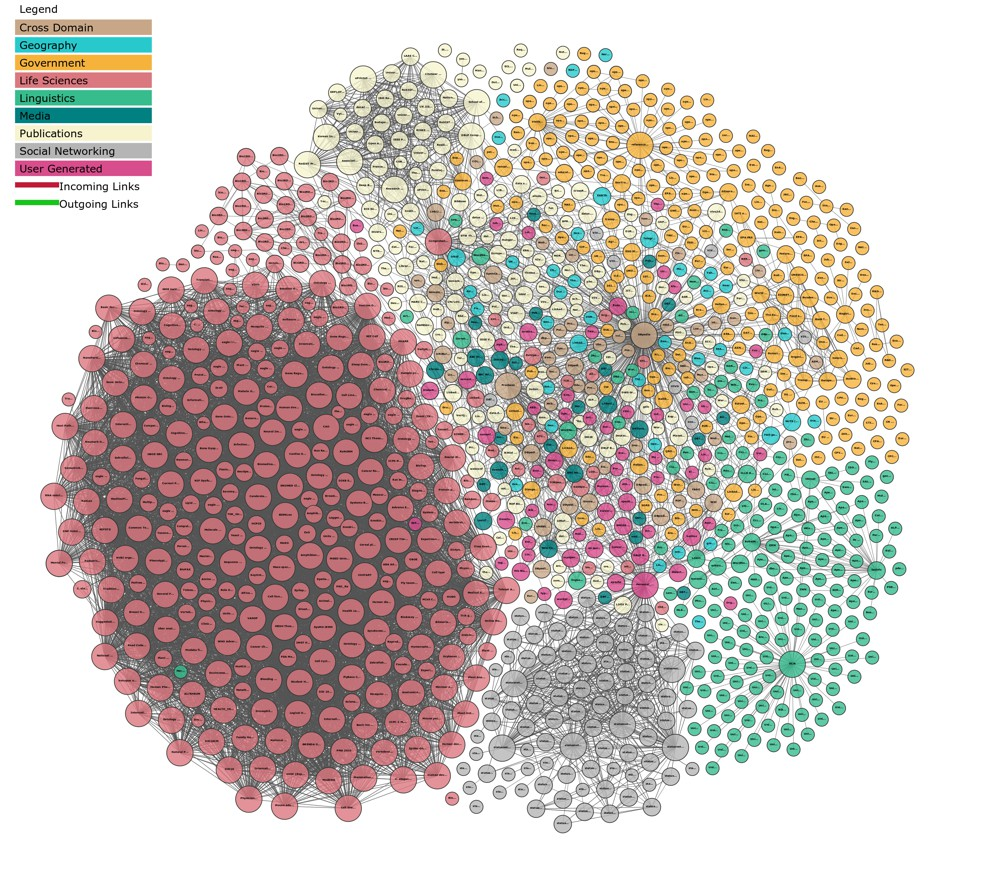
\includegraphics[scale=0.7]{imagens/lod_graph.png}
	\caption{Diagrama da nuvem dos dados ligados \citep{LODGraph}}
	\label{fig:lod-graph}
\end{figure}

\section{Similaridade Semântica}

A similaridade semântica entre dois termos, recursos, itens ou documentos é uma métrica para medir a distância de seus significados ou semântica, dado suas ontologias \citep{Slimani2013}. O objetivo é estabelecer características em comum entre dois conceitos. A distância entre dois conceitos para humanos pode não ter uma definição formal, já que se pode criar um juízo de valor diferente no relacionamento entre eles. Como exemplo, para uma pessoa a maçã e a banana podem estar mais relacionadas do que a maçã e a pera para outra. A similaridade e relação semântica podem por vezes serem determinadas como a mesma coisa, ambas como métricas de distâncias entre termos, contudo a similaridade semântica é mais específica \citep{Slimani2013}. A relação semântica é calculada usando um modelo de espaço vetorial e uma métrica de similaridade, como a similaridade do cosseno \ref{eq:cosine_sim} que dado dois vetores $A$ e $B$ como uma representação de dois documentos e $A_i$ e $B_i$ seus componentes, seja calculado o produto vetorial euclidiano. \citep{Singhal2001}.

\begin{equation}
	A \cdot B = \norm{A}_2 \norm{B}_2 \cos(\theta)
\label{eq:cosine_sim_eu}
\end{equation}

\begin{equation}
	similaridade = \cos(\theta) = \frac{ A \cdot B }{ \norm{A}_2 \cdot \norm{B}_2 }
	= \frac{ \sum_{i=1}^{n} A_i B_i }{ \sqrt{ \sum_{i=1}^{n} A_i^{2} } \sqrt{ \sum_{i=1}^{n} B_i^{2} } }
\label{eq:cosine_sim}
\end{equation}

Entretanto, para a similaridade semântica é levado em consideração relações léxicas de sinonímia e hiperonímia onde o significado é abrangido pelo outro termo mais geral (como carro e veículo) \citep{Gracia2008}. Na prática, a similaridade semântica pode ser medida pelo menor caminho entre dois termos utilizando suas ontologias associadas. Para calcular a similaridade podem ser usadas diversos tipos de ontologias. \cite{Slimani2013} descreve dois principais tipos de ontologias usadas para medir similaridade.

\begin{itemize}
	\item{\textbf{Propósito genérico}: \textit{Wordnet}\footnote{https://wordnet.princeton.edu} é um banco de dados que modela o conhecimento léxico da língua inglesa. Nomes, verbos, adjetivos e advérbios são agrupados em conjuntos sinônimos, onde cada um expressa um conceito distinto. Essa ontologia pode ser utilizada para criar um \textit{score} de similaridade. Pode ser considerada um ontologia para termos de linguagem natural.}

	\item{\textbf{De domínio específico}: \textit{ULMS}\footnote{https://www.nlm.nih.gov/research/umls} é um sistema de linguagem médica com uma rede semântica de ontologias de multiuso, multilíngue para biomedicina, conceitos e assuntos relacionados à saúde. O banco de dados do sistema possui uma coleção de vocabulários de conceitos e termos e seus relacionamentos que são denominados de \textit{Metathesaurus}. Cada Metathesaurus é classificado como pelo menos uma categoria semântica.}
\end{itemize}

\subsection{Medidas de Similaridade Semântica}

Na literatura já foram apresentadas algumas medidas de similaridade semântica, mas comumente existem três fatores principais \citep{Slimani2013} que podem ser associados na topologia (i.e. nós do grafo direcionado) das ontologias: \textit{path length}, \textit{depth}, \textit{density}. Todos esses fatores afetam a medida da distância semântica, assim como as características entre dois termos, que podem aumentar ou diminuir as medidas de acordo com suas semelhanças. Quanto a densidade entre dois termos trata-se do número de filhos dos quais pertencem ao menor caminho (\textit{path}) da raiz ao mais específico conceito entre esses termos. Os fatores que influenciam nas medidas levam a definição de uma classificação que podem ser divididas em quatro principais \citep{Slimani2013}: baseadas em estrutura, conteúdo, recursos ou características e as híbridas que combinam as características estruturais (\textit{path length}, \textit{depth}, \textit{density}) e alguma outra abordagem.

\subsubsection{Baseadas em estrutura}

As medidas baseadas em estrutura (\textit{Structured-based ou Path-based}, utilizam funções que computam a similaridade baseada na hierarquia e estrutura da ontologia, ou seja, onde um conceito é definido como “é parte de”, “é um” etc. A função calcula o tamanho do caminho que liga os termos e seus posicionamentos no grafo direcionado da ontologia. Quanto mais dois conceitos são similares, mais \textit{links} existem entre eles. Dentre as medidas baseadas em estrutura se destacam:

\begin{itemize}
	\item{\textbf{\textit{Shortest Path} \citep{Rada:1989}}: A medida do menor caminho é um tipo de medida de distância que é primariamente voltada para lidar com hierarquias em redes semânticas. A função da similaridade entre conceitos $C_1$ e $C_2$ é definida como:

	\begin{equation}
		Sim(C_1, C_2) = 2 * Max(C_1, C_2) - SP
	\label{eq:shortest_path}
	\end{equation}

	A função $Max$ é o maior tamanho do caminho entre $C_1$ e $C_2$, quanto a $SP$ é menor caminho relacionando os dois conceitos.}

	\item{\textbf{\textit{Weighted Links}}: Similar a medida do menor caminho, contudo é introduzido um conceito de pesos para os links entre os conceitos a serem comparados.}

	\item{\textbf{\cite{Wu:1994}}: Para essa medida sejam dois conceitos $C_1$ e $C_2$, é levado em consideração a noção intuitiva de que quanto maior a profundidade, mais similares os conceitos são. Na função tem-se que $N_1$ e $N_2$ são a quantidade de links da forma "é um" de $C_1$ e $C_2$, onde o conceito mais específico é o mais próximo ancestral  $C$ entre eles.

	\begin{equation}
		Sim_{W \& P}(C_1, C_2) = \frac{2H}{N_1 + N_2 + 2H}
	\label{eq:wu_palmer}
	\end{equation}	}
\end{itemize}

\subsubsection{Baseadas em conteúdo}

As medidas baseadas no conteúdo, são aquelas que utilizam a informação do conteúdo para medir similaridade. O conteúdo de um conceito é definido pela frequência de termos dado uma coleção de documentos. Grande parte das medidas deste tipo utilizam a informação compartilhada de dois conceitos pais $C_1$ e $C_2$, dos qual $S(C_1; C_2)$ é o conjunto de conceitos que os engloba, conforme a Equação \ref{eq:mis}.  O menor $p(C)$ é utilizado quando há mais de um pai em comum que $C$ é o \ac{MIS}, ou seja, o conceito mais informacional que os engloba.

	\begin{equation}
		P_{mis}(C_1, C_2) = min_{C \in S(C_1;C_2)} \{p(C)\}
	\label{eq:mis}
	\end{equation}

Algumas das medidas deste tipo são:

\begin{itemize}

	\item{\textbf{\cite{Resnik:1999}}: O principio desta medida define que dois conceitos são mais similares se eles possuem mais informações compartilhadas. A informação compartilhada entre $C_1$ e $C_2$ é o conteúdo de conceitos que os engloba no grafo. A definição de \textit{Resnik} define a medida como a seguinte equação:

	\begin{equation}
		Sim_{Resnik}(C_1, C_2) = - \ln (p_{mis}(C_1, C_2))
	\label{eq:resnik}
	\end{equation}}

	\item{\textbf{\cite{Lin1993PrincipleBasedPW}}: A proposta é incorporar o vetor semântico e a ordem das palavras para calcular a similaridade. A medida combina o menor caminho $SP$ entre dois conceitos e a profundidade $N$ da taxonomia em relação ao conceito $C$ mais em comum. A definição da equação segue conforme abaixo:

	\begin{equation}
		Sim_{Li}(C_1, C_2) = \mathrm{e}^{-\alpha * SP} * \frac{ \mathrm{e}^{\beta * N} - \mathrm{e}^{- \beta * N} }{ \mathrm{e}^{\beta * N} + \mathrm{e}^{- \beta * N} }
	\label{eq:li}
	\end{equation}}
\end{itemize}

\subsubsection{Baseadas em características ou recursos}

Baseia-se em características ou recursos (\textit{Featured-based}), que partem do princípio de valorizar informações importantes em relação ao conhecimento sobre um termo. A medida assume que os conceitos são descritos por termos indicando suas propriedades ou \textit{features}. A similaridade entre dois conceitos é definida por uma função (\ref{eq:tversky}) que relaciona suas propriedades ou relacionamentos a outros termos similares na hierarquia da ontologia. \cite{Tversky:1977} apresenta uma medida \textit{Feature-based} de termos para calcular a similaridade entre diferentes conceitos, contudo o posicionamento desses termos na taxonomia e a informação do conteúdo não são levadas em consideração. A proposta é de que com termos descritos por um conjunto de palavras como propriedades do conceito, então as que são em comum tendem a aumentar a similaridade, enquanto as que não são em tendem a diminuí-la. Dessa forma, é definida uma equação onde $C_1$ e $C_2$ representam o conjunto de descrições dos termos e $\alpha \in [0,1]$ é a relação de relevância das características que não são em comum. O valor de $\alpha$ aumenta o quão mais em comum dois conceitos são, e decresce com suas diferenças, e não é necessariamente uma relação de simetria, mas mais baseada na similaridade \citep{Slimani2013}.

\begin{equation}
	Sim_{Tversky}(C_1, C_2) = \frac{ |C_1 \cap C_2| }
	{ |C_1 \cap C_2| + \alpha |C_1 - C_2| + (\alpha - 1)|C_2 - C_1| }
\label{eq:tversky}
\end{equation}

\section{Projetos na Web Semântica}

\subsection{DBPedia}

A DBPedia (DB para \textit{database}) é um esforço colaborativo para a extração de dados do Wikipedia para publicação de dados essencialmente em RDF \citep{Auer:2007:DNW:1785162.1785216}. Um dos objetivos é possibilitar que outros explorem a criar uma experiência da enciclopédia mais abrangente, utilizando serviços e aplicações na Web Semântica. O projeto é um dos mais famosos que aplica os conceitos de dados ligados, onde sua importância não somente é dada pela publicação dos dados da Wikipedia, mas também da incorporação de links de outros \textit{datasets}. De fato, o DBpedia, por muitas vezes é considerado um núcleo dentro da iniciativa do LOD.

O projeto tem o foco em converter o conteúdo presente do Wikipedia em conhecimento estruturado utilizando as tecnologias da Web Semântica, para que outros agentes possam explorar realizando consultas e ligando a outros conjuntos de dados \citep{Auer:2007:DNW:1785162.1785216}. Assim, o projeto cobre uma das limitações da Wikipedia que é a dependência de apenas ter a busca em texto livre para encontrar informação. Desse papel, o projeto promove três importantes contribuições:

\begin{itemize}
	\item{Desenvolvimento de um \textit{framework} para extração de informação, o qual converte o conteúdo da Wikipedia em RDF.}

	\item{Prover o conteúdo da Wikipedia como um largo, multi-domínio \textit{dataset} de RDF. Já são cerca de 900 milhões de triplas mapeadas (2021). A Tabela \ref{tab:dbpedia-triples} mostra um recorte das entidades mapeadas do DBPedia.}

	\item{Interligar o DBpedia com outros conjuntos de dados abertos, o que expande a contagem das triplas RDF para mais de bilhão.}

	\item{Desenvolvimento de uma série de interfaces e módulos de acesso para que tal \textit{dataset} possa ser acessado por serviços da Web ligado a outros sites.}
\end{itemize}

\begin{table}[]
\centering
\resizebox{\textwidth}{!}{%
\begin{tabular}{|l|r|r|r|r|r|r|}
\hline
\multicolumn{7}{|c|}{\textbf{Amostra de Dados do DBPedia}}                                                                                                                                                                                                            \\ \hline
                       & \multicolumn{6}{c|}{\textbf{Línguas}}                                                                                                                                                                                                        \\ \hline
\textbf{Instâncias}    & \multicolumn{1}{l|}{\textbf{Inglês}} & \multicolumn{1}{l|}{\textbf{Espanhol}} & \multicolumn{1}{l|}{\textbf{Português}} & \multicolumn{1}{l|}{\textbf{Francês}} & \multicolumn{1}{l|}{\textbf{Alemão}} & \multicolumn{1}{l|}{\textbf{Russo}} \\ \hline
Pessoas                & 1.445.104                            & 99.147                                 & 60.056                                  & 134.749                               & 179.421                              & 86.269                              \\ \hline
Atores                 & 6.501                                & 13.831                                 & 7.546                                   & 14.019                                & 0                                    & 0                                   \\ \hline
Artistas               & 96.282                               & 34.898                                 & 14.603                                  & 32.562                                & 0                                    & 30.266                              \\ \hline
Políticos              & 40.343                               & 7.460                                  & 4.110                                   & 11.461                                & 0                                    & 0                                   \\ \hline
Lugares                & 735.062                              & 156.377                                & 123.114                                 & 148.586                               & 168.082                              & 91.099                              \\ \hline
Instuições de   ensino & 49.172                               & 1.709                                  & 514                                     & 2.943                                 & 2.600                                & 1.418                               \\ \hline
Filmes                 & 87.282                               & 12.140                                 & 11.643                                  & 15.669                                & 18.707                               & 14.912                              \\ \hline
Livros                 & 31.029                               & 2.217                                  & 1.343                                   & 3.549                                 & 0                                    & 18.491                              \\ \hline
Software               & 31.401                               & 6.284                                  & 4.245                                   & 8.980                                 & 5.286                                & 0                                   \\ \hline
\end{tabular}%
}
\caption{Recorte da tabela de dados de triplas de entidades mapeadas no DBPedia. \citep{DBPedia:2014}}
\label{tab:dbpedia-triples}
\end{table}

\begin{figure}
	\centering
	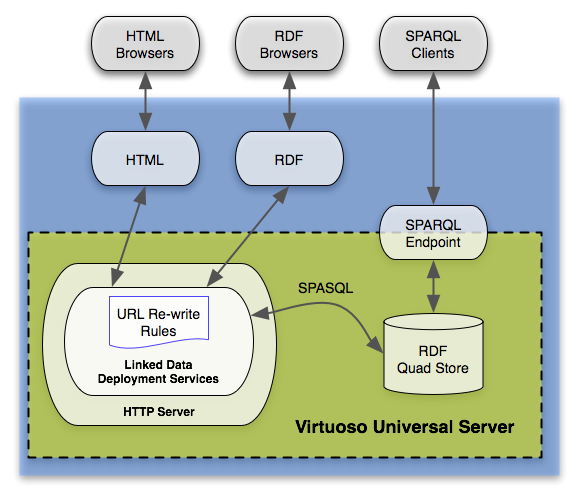
\includegraphics[scale=0.55]{imagens/dbpedia_virtuoso.png}
	\caption{Ilustração da arquitetura do DBPèdia \citep{DBPediaVirtuoso}}
	\label{fig:dbpedia-virtuoso}
\end{figure}

Como a iniciativa compõe o movimento do LOD, os dados do DBpedia podem ser importados por aplicações \textit{third party} utilizando a licença aberta. O projeto faz uso da plataforma do \textit{Virtuoso Universal Server}\footnote{https://virtuoso.openlinksw.com} para prover os dados de RDFs através de uma interface e um \textit{endpoint} em SPARQL. Na Figura \ref{fig:dbpedia-virtuoso} é apresentado um panorama da arquitetura do projeto.

\subsection{Google Knowledge Graph}

O \textit{Knowledge Graph} é uma base de conhecimento desenvolvida pelo Google\footnote{https://www.google.com} para melhorar e ampliar seu mecanismo de busca \citep{GoogleKnowledge}. Alinhado aos objetivos da Web Semântica, o projeto pretende expandir o buscador com um grafo de conhecimento, onde foi mapeado entidades de dados legíveis para máquinas com o intuído recuperar a informação semântica nos termos buscados. De forma simples, o intuito é ter a informação de coisas e não de \textit{strings}. Como exemplo, ao ser buscado a palavra "leão", não será apenas retornado uma lista de sites que possuem referências a palavra, mas também prover a semântica e taxonomias envolvidas com a ontologia e relacionados.

\begin{figure}
	\centering
	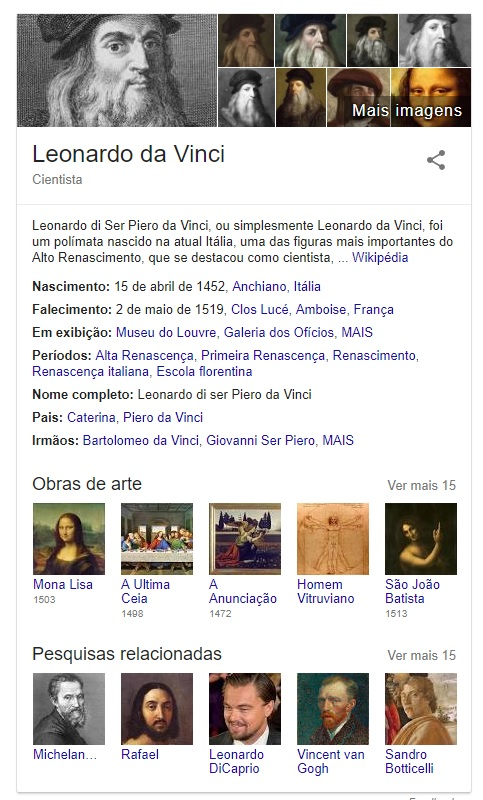
\includegraphics[scale=0.8]{imagens/knowledge_graph.jpg}
	\caption{Ilustração do sumário de dados mapeados no Google Knowledge Graph.}
	\label{fig:knowledge-graph}
\end{figure}

Com \textit{Knowledge Graph} é possível pesquisar por pessoas, lugares, esportes, filmes e diversas informações que o Google mapeou no grafo do conhecimento. O serviço já conta com mais de 500 milhões de objetos e 3.5 bilhões de fatos sobre o relacionamento entre diferentes objetos. O objetivo do Google é ampliar o mecanismo de busca em três sentidos: Possibilitar encontrar o item certo, obter um melhor sumário, ser mais amplo e profundo. Um dos primeiros passos da companhia para atingir os objetivos do projeto é a construção do painel do sumário. Quando pesquisamos por \textit{Leonardo Da Vinci}, procurando seja pelas suas pinturas ou por pintores da renascença, o sistema montará um quadro de dados, conforme a Figura \ref{fig:knowledge-graph} com as informações, além trazer itens com relações próximas, como seus quadros e outros artistas relacionados. Com esse tratamento \cite{GoogleKnowledge} alega que será possível melhor compreender o que os usuários buscam, além de dar importantes passos para migrar de um motor informação para um de conhecimento, algo importante para o uso em seus assistentes virtuais.

\section{Sumário}

Neste capítulo, foi apresentado os conceitos que fundamentam o desenvolvimento de sistemas para representação de conhecimentos, assim como a abordagem e objetivos da Web Semântica sobre o tema. Em sequência foram introduzidas as principais tecnologias e princípios que são utilizados e o aprofundamento do significado das ontologias. Também foi abordado um panorama sobre a estrutura das tecnologias utilizadas na Web Semântica. Ainda foi introduzido o princípio e prática dos dados ligados e sua extensão com os dados abertos. Ainda foi exposto um panorama da similaridade semântica e tipos de medidas. Por fim, foram apresentados projetos proeminentes no cenário da Web Semântica. No capítulo \ref{cap:proposal} será discutido os conceitos da proposta do sistema de recomendação implementados neste trabalho.

\chapter{Recomendação com similaridade semântica ponderada por links de recursos na DBPedia}
\label{cap:proposal}

\begin{quotation}[]{Steve Jobs}
You can't connect the dots looking forward; you can only connect them looking backwards. So you have to trust that the dots will somehow connect in your future.
\end{quotation}

Desde tempos o homem busca construir ferramentas e máquinas que ampliem e sustem sua capacidade de trabalho e produção. Com o advento dos programas de máquina, o \textit{software} tornou-se essencial para a demanda de problemas e desafios população. Como avaliado por \citep{Sommerville2010}, o software não se restringe a propriedades materiais das leis da física ou por processos de manufatura, o que por um lado simplifica a engenharia de software devido falta de restrições físicas, mas por outro, o torna complexo e custoso para mudanças. Assim, com a crescente quantidade e diversidade de computadores e dispositivos, é cada vez mais relevante a qualidade de software, visando a legibilidade, manutenção e evolução.

Neste capítulo serão apresentados os conceitos para a criação de sistema de recomendação com similaridade semântica ponderada por links de recursos na DBPedia\footnote{http://wiki.dbpedia.org}, sendo baseado nas preferências do usuário. Serão discutidas as tecnologias, arquiteturas, modelos dos dados, recomendação e algoritmos.

\section{Arquitetura}

Na arquitetura do sistema proposto, existe uma camada que é responsável pela construção das recomendações que possui os seguintes principais serviços:

\begin{itemize}
	\item{\textbf{Geração de Tokens}: Um dos objetivos do sistema é recomendar itens baseando-se no conteúdo não estruturado, no caso a sinopse dos filmes. A primeira tarefa é extrair as palavras, os \textit{tokens} relevantes dos textos, como nomes, adjetivos, lugares, entre outras, utilizando o processo de \ac{NLP}.}

	\item{\textbf{Cálculo da métrica de similaridade}: Após a geração das palavras importantes dos filmes, o sistema deve possuir um serviço para realizar o cálculo da similaridade entre dois tokens quaisquer, tirando proveito dos serviços da Web Semântica, no caso o DBPedia. Mais a frente será apresentada a equação da similaridade construída para este projeto, conforme consta na seção \ref{ssec:sim_rec}.}

	\item{\textbf{Geração das recomendações}: No último serviço, o sistema deverá construir um modelo dados através da geração de tokens para comparar as preferências do usuário com um filme, utilizando a métrica de similaridade proposta. Na seção \ref{sec:dataModel} é apresentado como é construído esses modelos e na seção \ref{ssec:sim_rec} o método utilizado para gerar a comparação e prover as recomendações.}
\end{itemize}

\section{Processo de Recomendação}

A proposta é criar uma recomendação baseada em conteúdo, ou seja, nos interesses que o usuário demonstrou no passado. A \textit{feature} analisada nos itens a serem avaliados, trata-se de um conteúdo não estruturado, no caso a descrição do item. Para este trabalho foi definido o domínio de filmes como exemplo de utilização, sendo assim, utilizando o texto da sinopse dos filmes como base para recomendação. A seguir será apresentado todas as etapas desde a captura dos dados até a apresentação das recomendações.

\begin{figure}
	\centering
	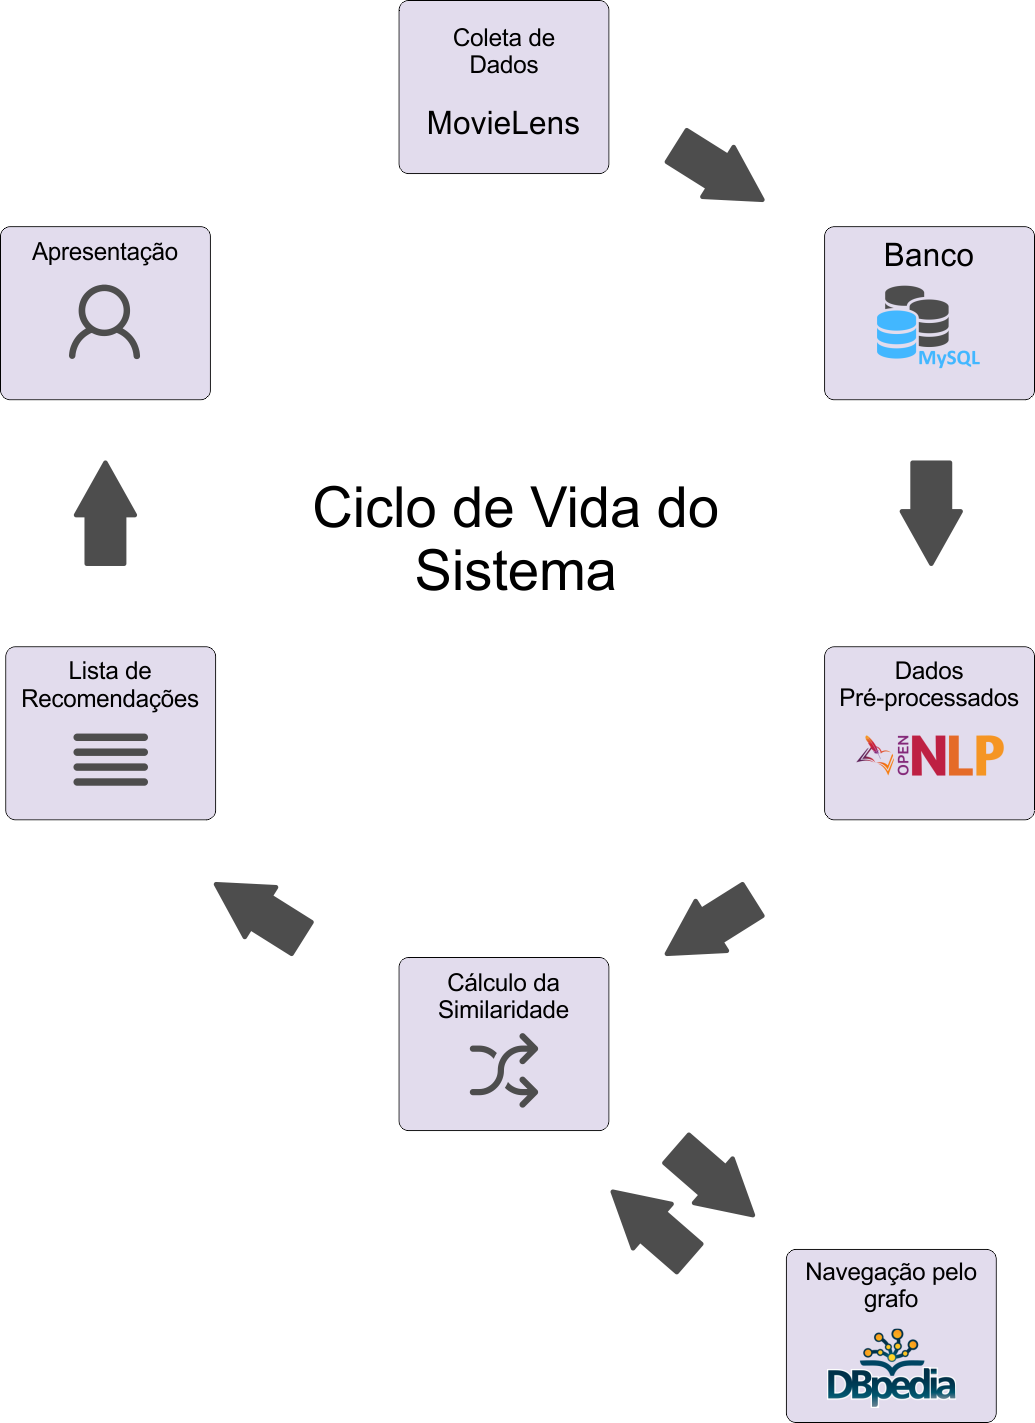
\includegraphics[scale=0.42]{imagens/recsys_fluxo.png}
	\caption{Fluxo das camadas do sistema de recomendação.}
	\label{fig:recsys_fluxo}
\end{figure}

\begin{enumerate}
	\item{\textbf{Coleta dos filmes}: Serão coletados dados dos filmes utilizando o projeto MovieLens\footnote{https://movielens.org} (ver \ref{sec:dataModel}).}

	\item{\textbf{Pré-processamento dos filmes}: Nessa etapa após a coleta dos filmes, os dados serão previamente processados para a geração de \textit{tokens} com \ac{NLP}, analisando a descrição dos itens (sinopse dos filmes). Após processados os \textit{tokens} serão persistidos no banco de dados.}

	\item{\textbf{Coleta das preferências do usuário}: Serão coletadas as avaliações dos usuários pelo projeto MovieLens, podendo assim montar um perfil de preferências.}

	\item{\textbf{Cálculo da Similaridade}: Após a etapa de pré-processamento dos filmes, será realizado o cálculo da similaridade entre os tokens do modelo do usuário e do filme, utilizando o métrica proposta \ac{RLWS}.}

	\item{\textbf{Geração das recomendações}: De posse do cálculo da similaridade, será gerado um conjunto de tamanho qualquer com os melhores \textit{scores} obtidos do cálculo desta similaridade. Posteriormente essa coleção filmes sugeridos será armazenada no banco, podendo ser atualizada conforme o perfil do usuário altera, ou novos filmes são cadastrados na base de dados. Na seção \ref{ssec:sim_rec} é demonstrado e discutido o algoritmo central para a similaridade e recomendação.}

	\item{\textbf{Apresentação dos resultados}: Por fim o sistema apresentará os resultados das recomendações para o usuário.}
\end{enumerate}

A Figura \ref{fig:recsys_fluxo} mostra como esse fluxo de funcionalidades é operado por todo o sistema. A seguir será o modelo dados elaborado para este trabalho.

\section{Modelo de dados}
\label{sec:dataModel}

Para a estrutura do sistema de recomendação foi elaborado um modelo de dados para o usuário, levando em conta suas preferências, além do modelo para as informações dos filmes. Nesta seção serão apresentados como os dados estão estruturados no banco de dados, além de estabelecer um modelo formal para o usuário e o filme, prontos para serem executado pelos camada de recomendação.

\subsection{Banco de dados}

Para trabalhar com as informações dos usuários e dos filmes, permitindo criar seus modelos para recomendação, os dados foram modelados e organizados de tal forma que possam ser facilmente persistidos e recuperados assim que necessário. A Figura \ref{fig:user_model} mostra como esses dados estão estruturados e interligados. É importante ressaltar algumas observações quanto a essa estrutura:

\begin{itemize}
	\item{A entidade \textit{rating} persiste as avaliações dos usuários, medidas de 0 a 5. Desta entidade será construída as preferências do usuário, ou seja, extraídos aqueles filmes que possuem boas avaliações refletindo aquilo que o usuário tem interesse.}

	\item{A entidade \textit{recomendation} persiste as sugestões de filmes calculadas pelo sistema, e o atributo \enquote{similarity} trata-se do algoritmo de similaridade utilizado, o que torna-se especialmente útil para realizar comparações com outros métodos (será discutido no \ref{cap:evaluation}).}

	\item{A entidade \textit{movie} persiste os dados dos filmes retirados do projeto MovieLens\footnote{https://movielens.org}, assim como o processamento da sinopse dos filmes para geração dos \textit{tokens}.}

	\item{A entidade \textit{idf} persiste o cálculo do \ac{IDF} da Equação \ref{eq:tfidf}, que servirá para o cálculo da similaridade cosseno, por motivos de comparação que serão discutidos no \ref{cap:evaluation}.}

	\item{As entidades \textit{lod\_cache} e \textit{lod\_cache\_relation} tratam-se do serviço de cache para o cálculo da similaridade, assim poupando tempo para consultas do serviço do DBPedia. Na seção \ref{sec:cache} a estrutura de cache dos sistema é melhor abordada.}
\end{itemize}

\begin{figure}
	\centering
	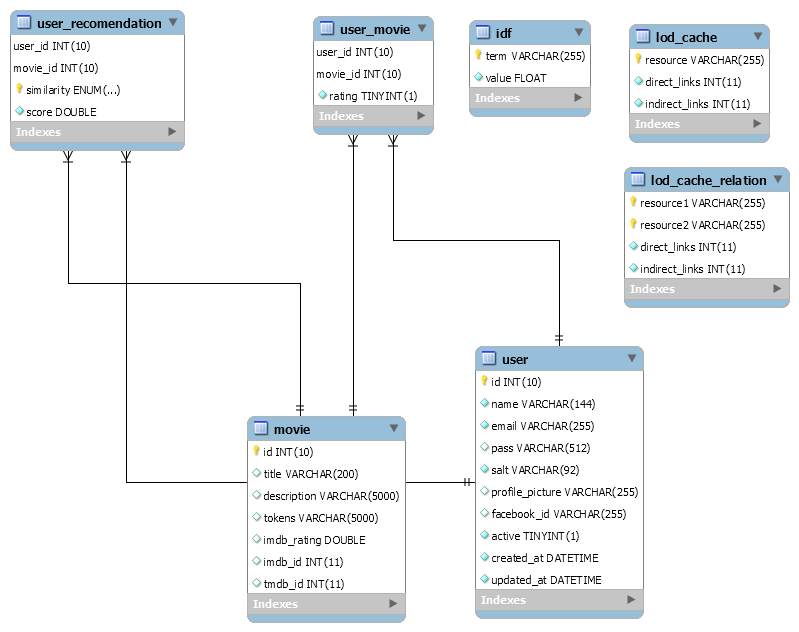
\includegraphics[scale=0.5]{imagens/user_model.png}
	\caption{Diagrama da modelagem dos dados extraído do banco MySQL}
	\label{fig:user_model}
\end{figure}

\label{ssec:database}
\subsection{Modelo de filmes}

Com a estrutura de dados utilizada para os filmes, é importante também formalizar como é seu modelo na recomendação, afinal este é o item a ser recomendado para o usuário. É definido um conjunto $X$ como sendo conjunto de todos os filmes, onde cada filme $F \subset X$ é um conjunto de tokens únicos $t_f$ extraídos pelo processo de \ac{NLP} (ver seção \ref{ssec:data_nlp}) através da sinopse deste. Para simplificar a formalização dos modelos, nota-se que o conjunto de termos $F$ do filme representa o filme junto com seus metadados, conforme definido em \ref{ssec:database}.

Desda forma formaliza-se o modelo de filmes conforme mostra as equações \ref{eq:film_model} e \ref{eq:film_model2}.

\begin{equation}
	X = \bigcup\limits_{i=1}^{\infty} F_{i}
\label{eq:film_model}
\end{equation}

\begin{equation}
	F = \{t_{f_1}, ..., t_{f_n} \; | \; 1 \leq n \leq \mathbb{N}^*\}
\label{eq:film_model2}
\end{equation}

\subsection{Modelo de usuários}
\label{ssec:user_model}

Os usuários inicialmente são estruturados como um conjunto de filmes, sendo extraídos aqueles bem avaliados por ele, à partir de uma nota de relevância $r$ baseada num modelo de cinco estrelas, onde nenhuma estrela é totalmente irrelevante e cinco totalmente relevante. Os filmes bem avaliados serão aqueles com relevância $r \geq 3,5$, portanto sendo suas preferências. Contudo, desta forma ainda não é possível realizar a comparação com o modelo de filmes utilizando a métrica de similaridade proposta (ver \ref{ssec:sim_rec}), devido a comparação ser de termo a termo. Uma opção inicial seria simplesmente calcular todos os termos dos filmes de preferência do usuário, utilizado no processo de \ac{NLP}, e uni-los num grande conjunto, porém isto tornaria o modelo de usuário muito custoso para ser utilizado, além de não escalar bem conforme as preferência do usuário aumentam. Sendo assim, optou-se por calcular os \enquote{melhores termos únicos} que representam o usuário, como sendo um conjunto de termos de um tamanho definido. Para calcular esses \enquote{melhores termos} é aplicado um modelo de frequência, o \ac{TFIDF} (ver Equação \ref{eq:tfidf}), que busca criar um ranking de termos determinando o quão importante são numa coleção, no caso a união de todos os conjuntos filmes e seus termos. Com isso é definido $Y$ como sendo o conjunto de todos os usuários $U$, e este por sua vez a união de todos os filmes $F_u$ e $P$ um subconjunto com aqueles de sua preferência, contendo todos os termos. Esses termos são denominados de termos do usuário, representado pelo elemento $t_u$. Assim como o modelo de filmes, os conjuntos $U$ e $P$ de termos do usuário também representa seus metadados. Posteriormente, define-se o conjunto $M_u$ sendo o \textbf{modelo do usuário} dos melhores termos $t_u \in P$, ao passarem pela seleção da função $M_{tfidf}$, que um define um subconjunto de um tamanho definido pela constante $z$. Por fim, o conjunto $Z$ é a união de todos os modelos de usuário $M_u$. O tamanho de $M_u$ será explorado no capítulo \ref{cap:evaluation}. As equações \ref{eq:user_model1} à \ref{eq:user_model5} formalizam a construção do modelo do usuário.


\begin{equation}
	Y = \bigcup\limits_{i=1}^{\infty} U_i \quad \text{ (todos os usuários)}
\label{eq:user_model1}
\end{equation}

\begin{equation}
	U = \bigcup\limits_{i=1}^{\infty} F_{u_i} \quad \text{ (todos os filmes do usuário)}
\label{eq:user_model2}
\end{equation}

\begin{equation}
	\begin{aligned}
		P = \bigcup\limits_{i=1}^{\infty} F_{u_i} \quad \{F_{u_i} \;|\; 3,5 \leq r \leq 5 \;\;\land\;\; r \in \mathbb{R} \;\;\land\;\; \frac{r}{0,5} \in \mathbb{N}\}\\
		\text{(todos os filmes de preferência do usuário)}
	\end{aligned}
\label{eq:user_model3}
\end{equation}

\begin{equation}
	\begin{aligned}
		(\forall t_u \in F_u \;\land\; F_u \subset P) \quad M_u = \{t_u \;| \; M_{tfidf}(P, z), \; |M_u| = z \; \land \; z \in \mathbb{N}^*\} \\
		\text{ (aplicação dos melhores termos do usuário)}
	\end{aligned}
\end{equation}

\begin{equation}
	Z = \bigcup\limits_{i=1}^{\infty} M_{u_i} \quad \text{ (todos os modelos de usuários)}
\label{eq:user_model5}
\end{equation}

\subsection{Preparação dos dados para recomendação}
\label{ssec:data_nlp}

Antes da execução das recomendações é necessário realizar a etapa do pré-processamento dos dados. Para cada filme são gerados \textit{tokens} que são palavras relevantes presentes na descrição. Essas palavras relevantes tratam-se do processo de exclusão daquelas que pouco agregam significado ao que se refere a temática do filme, como é o exemplo de preposições, conjunções e artigos.

Para extração dessas palavras, foi utilizado o processo denominado de \ac{NLP} que envolve uma série de tarefas para o processamento de linguagens naturais \footnote{Linguagem desenvolvida naturalmente pelo ser humano de forma não premeditada, no caso a escrita}, para compreensão e interação entre máquinas e humanos, conforme é apresentado por \cite{Collobert:2011}. A Figura \ref{fig:nlp} ilustra as tarefas comuns no processamento de linguagem natural. O foco é extrair dos termos palavras com fortes significados, como adjetivos, verbos, além de também identificar substantivos, inclusive os compostos. Abaixo consta as tarefas que foram utilizadas para no processo de preparação dos dados:

\begin{itemize}
	\item{\textbf{Tokenization}: Esta tarefa consiste em segmentar um texto em partes da linguagem, sendo responsável por criar separar em tokens. Muitas vezes também é utilizado o processo de \textit{chunking} que visa ir além de separar as palavras mas segmentar o texto em frases em partes maiores do texto, algo que não foi utilizado neste projeto.}
	\item{\textbf{Tagging, \ac{POS}}: O objetivo desta tarefa é reconhecer as palavras do processo de tokenization como "partes do discurso", criando \textit{tags} para identificar o que elas representam na linguagem. Nesta parte é onde se classificam as palavras em verbos, adjetivos, substantivos, pontuações etc.}
	\item{\textbf{\ac{NER}}: Esta tarefa objetiva reconhecer nas palavras e tokens aquelas que tratam-se de nomes próprios, além de associá-las à algum tipo, como pessoas, lugares, moedas etc.}
\end{itemize}

\begin{figure}
	\centering
	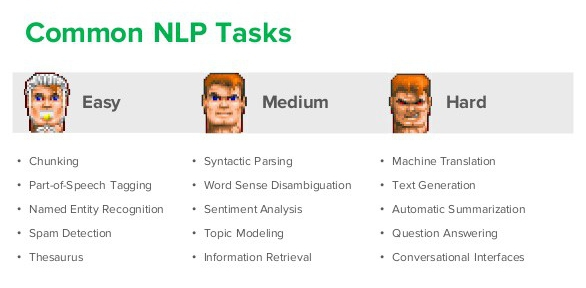
\includegraphics[scale=0.70]{imagens/nlp.jpg}
	\caption{Segmentação de tarefas no NLP. \citep{NLP2016}}
	\label{fig:nlp}
\end{figure}

Para facilitar a execução dessas tarefas do \ac{NLP}, optou-se por utilizar o \textit{framework} OpenNLP\footnote{https://opennlp.apache.org}, conforme também abordado na seção \ref{ssec:open_nlp}, que através de um modelo de treinamento, possibilita facilmente realizar o processo de \textit{tagging}, identificando as partes do discurso. Uma vez realizada a anotação do texto definiu-se apenas capturar as palavras marcadas com as \textit{tags} conforme mostra a tabela \ref{tab:nlp_tags}. Vale ressaltar que essas definições foram concebidas para língua inglesa, uma vez que as sinopses importadas do projeto MovieLens\footnote{https://movielens.org} estão nessa língua.

Em seguida é incluído ao conjunto de termos os tokens da tarefa \ac{NER}, o que não é meramente o reconhecimento de nomes próprios do texto, mas também de nomes compostos. Esse processo é de grande valia para a etapa de similaridade uma vez que tendo um nome como "Buzz Lightyear", apenas utilizando o processo da marcação das partes do discurso, resultaria em dois termos "Buzz" e "Lightyear", sendo que o ideal seja também ter o nome composto por inteiro. Os substantivos próprios obtidos pelo processo \ac{POS} também são mantidos no conjunto de termos, uma vez que o framework utilizado no processo de \ac{NLP} apenas extrai, nomes, lugares e organizações. Para os nomes reconhecidos nesse processo também foi realizada uma formatação para adequação à consultas \ac{SPARQL}, ou seja, nomes compostos como "Buzz Lightyear" são formatados para "Buzz\textunderscore Lightyear", mantendo as iniciais maiúsculas e separando as palavras por "\textunderscore" . A tabela \ref{tab:nlp_example} demonstra alguns exemplos do tratamento da descrição de filmes para geração de \textit{tokens}.

\begin{table}[H]
	\centering
	\caption{Relação das tags das partes do discurso}
	\def\arraystretch{1.3} % padding da linhas da tabela
	\begin{tabular}{| m{1.3cm} | m{9.4cm}| c | m{2cm}}
		\hline
		\multicolumn{1}{|c|}{\bfseries Tag} & \multicolumn{1}{c|}{\bfseries Descrição} \\ \hline
		NN & Substantivo comum, singular ou incontável \\ \hline
		NNS	& Substantivo comum, plural \\ \hline
		NNP	& Substantivo próprio, singular \\ \hline
		NNPS & Substantivo próprio, plural \\ \hline
		JJ & Adjetivo \\ \hline
		JJR & Adjetivo comparativo \\ \hline
		JJS & Adjetivo superlativo \\ \hline
		FW & Palavra estrangeira \\ \hline
		VB & Verbo, forma base \\ \hline
	\end{tabular}
\label{tab:nlp_tags}
\end{table}

\begin{table}[H]
	\centering
	\caption{Exemplos da geração de tokens}
	\def\arraystretch{1.3} % padding da linhas da tabela
	\begin{tabular}{|p{2cm}|p{6cm}|p{6cm}|}
	\hline
	\textbf{Filme} & \textbf{Sinopse} & \textbf{Tokens} \\ \hline
	Toy Story & Led by Woody, Andy's toys live happily in his room until Andy's birthday brings Buzz Lightyear onto the scene. Afraid of losing his place in Andy's heart, Woody plots against Buzz. But when circumstances separate Buzz and Woody from their owner, the duo eventually learns to put aside their differences.& Woody, Andy, Toys, Room, Andy, Birthday, Scene, Place, Andy, Heart, Woody, Plots, Circumstances, Woody, Owner, Duo, Put, Differences, Buzz\_Lightyear \\ \hline
	GoldenEye & James Bond must unmask the mysterious head of the Janus Syndicate and prevent the leader from utilizing the GoldenEye weapons system to inflict devastating revenge on Britain. & Unmask, Mysterious, Head, Janus, Syndicate, Prevent, Leader, Goldeneye, Weapons, System, Inflict, Devastating, Revenge, Britain, James\_Bond \\ \hline
	\end{tabular}
\label{tab:nlp_example}
\end{table}

\section{Modelo de Recomendação}
\label{ssec:sim_rec}

A criação de um modelo de recomendação envolve sugerir novos itens, sendo caracterizada como uma predição de o quão provável o usuário terá interesse no conteúdo recomendado. Nesta seção serão apresentadas as etapas que existem para construção deste modelo, que envolve a definição da métrica de similaridade, através da equação da similaridade semântica (ver \ref{ssec:formula_rlws}) e da construção da recomendação (ver \ref{ssec:rec_alg}).

Conforme abordado no capítulo \ref{cap:semantic_web}, a similaridade semântica utiliza e retira proveito das estruturas de uma ontologia que neste caso trata-se das acessíveis através do DBPedia\footnote{http://wiki.dbpedia.org}. Cada termo de um filme será considerado como um potencial recurso na DBPedia, e os recursos tratam-se de entidades de ontologias mapeadas no grafo dos princípios do \ac{LOD}. Diante disso, a métrica proposta é estabelecer uma equação de similaridade, utilizando-se de um modelo que considera a estrutura desses recursos, analisando a quantidade de relações e links diretos ou indiretos entre tais recursos. Para estabelecer a equação proposta, considerou-se dois trabalhos relacionados com similaridade semântica, o de \cite{PassantLDSD} que apresenta a equação \ac{LDSD}, e mais recentemente de \cite{PiaoResim}, que propõem o \ac{RESIM}. O primeiro trabalho tenta estabelecer a importância que um recurso tem em relação ao total de relações da união de dois recursos, sem preferências entre links diretos e indiretos, enquanto que \cite{PiaoResim} estende e modifica esse entendimento criando uma média ponderada entre as relações dos recursos e a similaridade entre suas propriedades.

Este trabalho propõe um novo método denominado de \ac{RLWS}, para realizar a medida da similaridade entre dois recursos presentes no DBPedia, criando uma média ponderada entre a relevância dos links diretos e indiretos, para gerar um valor na escala de 0 a 1, onde valores menores denotam menor similaridade.

\subsection{Equação para similaridade semântica}
\label{ssec:formula_rlws}

A Equação \ref{eq:rlws} demonstra o cálculo da similaridade semântica, que consiste em um conjunto de 5 funções  $C_d$, $C_i$, $C_{di}$, $C_{do}$, $C_{io}$. Estas funções tratam-se de levar em consideração a quantidade links de um recurso ou entre recursos dentro de um conjunto seguindo os princípios do \ac{LOD}, de acordo com a seguinte definição \citep{PiaoResim}:

\begin{definition}
Um conjunto que segue os princípios LOD é um grafo $G$ tal que $G = (R, L, I)$ aonde $R = \left\{r_1, r_2, ..., r_n\right\}$ é um conjunto de recursos identificados por suas URI, $L = \left\{i_1, i_2, ..., i_n\right\}$ é um conjunto de instâncias desses links entre recursos, como $i_i = <l_j, r_a, r_b>$.
\end{definition}

\begin{equation}
	RLWS(r_a, r_b) =
	\begin{dcases*}
		1 \text{,} \;\; URI(r_a) = URI(r_b) \;\; \text{ou} \;\; r_a \; \textit{ dbo:wikiPageRedirects } \; r_b\\
		\frac{S_d(r_a, r_b) * w_d + S_i(r_a, r_b) * w_i}{w_d + w_i}, \; \text{caso contrário}
	\end{dcases*}
\label{eq:rlws}
\end{equation}

\begin{equation}
	S_d(r_a, r_b) = 1 - \frac{1}{1 + \frac{\sum_i C_{di}(l_i, r_a, r_b) + \sum_i C_{do}(l_i, r_a, r_b)}{1 + \log (C_d(r_a) + C_d(r_b))}}
\label{eq:rlws_ex1}
\end{equation}

\begin{equation}
	S_i(r_a, r_b) = 1 - \frac{1}{1 + \frac{\sum_i C_{ii}(l_i, r_a, r_b)}{1 + \log (C_i(r_a) + C_i(r_b))}}
\label{eq:rlws_ex2}
\end{equation}

\begin{figure}
	\centering
	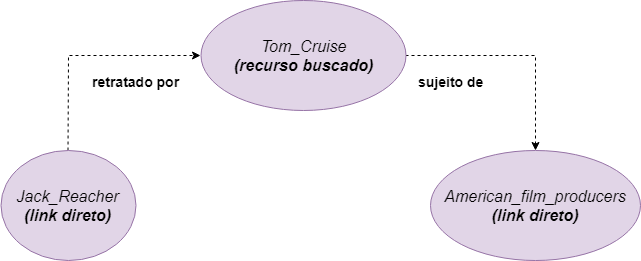
\includegraphics[scale=0.4]{imagens/cd_links.png}
	\caption{Imagem que retrata os links diretos saintes e entrantes de um recurso.}
	\label{fig:cd_links}
\end{figure}

A equação possui um condicional que implica o valor 1 quando dois recursos comparados tenham a mesma \textit{URI} ou estejam relacionados pela propriedade \textit{dbo:wikiPageRedirects}. Essa propriedade nada mais trata de redirecionamentos do próprio serviço do DBPedia, que quando consultando recursos como "Movie" e "Film", resultam na mesma página, pois são redirecionamentos. Para maior generalização o termo "link" será utilizado para se referir tanto a ligações como recursos ou propriedades relacionadas. As funções $C_d$ e $C_i$ tratam-se de computar os links distintos de um recurso qualquer, ou seja todas as ligações distintas a outros recursos, de forma direta e indireta respectivamente. No caso da função $C_d$, são computados todos os recursos distintos que sejam alcançados por uma propriedade qualquer através de um recurso analisado em questão, mais aqueles que partem de outro recurso e chegam nesse mesmo desejado. O exemplo da Figura \ref{fig:cd_links} apresenta o recurso "Tom\_Cruise" a ser calculado, que possui um link direto sainte para o recurso "American\_film\_producers" através da propriedade "sujeito de", e outro link direto de entrada pelo recurso "Jack\_Reacher" através da propriedade "retratado por".

\begin{lstlisting}[caption=Consulta SPARQL para contagem de links diretos, language=SQL, frame=single, label={cod:sparql_cd}, float, numbers=left]
PREFIX  :  <http://dbpedia.org/resource/>
PREFIX  dbo:  <http://dbpedia.org/ontology/>
SELECT (count (distinct ?p1) as ?x)
WHERE {
	{values (?r1) {(<http://dbpedia.org/resource/r1>)} ?r1 ?p1 ?r2 . FILTER (?r1 != ?r2)}
	UNION
	{values (?r1) {(<http://dbpedia.org/resource/r1>)} ?r2 ?p1 ?r1 . FILTER (?r1 != ?r2)}
	FILTER ( ?p1 != dbo:wikiPageID )
	FILTER ( ?p1 != dbo:wikiPageRevisionID )
	FILTER ( ?p1 != dbo:wikiPageRedirects )
	FILTER ( ?p1 != dbo:wikiPageExternalLink )
	FILTER ( ! isLiteral(?r2) )
}
\end{lstlisting}

A contagem desses links é realizada através da consulta \ac{SPARQL} conforme a Figura \ref{fig:cd_links}. Alguns filtros de propriedades são realizados, pois não são relevantes para a consulta. A propriedade \textit{dbo:wikiPageRedirect} é realizada por outra consulta a parte, mas é adicionada no filtro, para não levá-la em consideração durante a contagem. Para a função $C_i$ apenas são contabilizados os links indiretos de saída, por motivos de desempenho de consultas SPARQL no DBPedia. A imagem \ref{fig:ci_links} retrata o cenário para os links indiretos, e o Código \ref{cod:sparql_ci} a contagem dos links indiretos. Quanto para as funções $C_{di}$, $C_{do}$ e $C_{io}$, referem-se a contagem dos links distintos compartilhados entre dois recursos, sendo os dois primeiros de forma direta e o último de forma indireta. Os Códigos \ref{cod:sparql_cdio} e \ref{cod:sparql_cio} apresentam as consultas \ac{SPARQL} para realizar a contagem dos links.

\begin{figure}
	\centering
	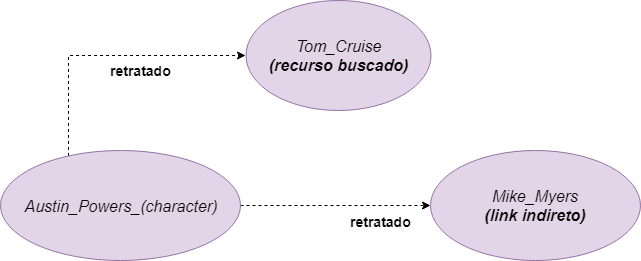
\includegraphics[scale=0.5]{imagens/ci_links.png}
	\caption{Imagem que retrata os links indiretos saintes de um recurso.}
	\label{fig:ci_links}
\end{figure}

\begin{lstlisting}[caption=Consulta SPARQL para contagem de links indiretos., language=SQL, frame=single, label={cod:sparql_ci}, float, numbers=left]
PREFIX  :  <http://dbpedia.org/resource/>
PREFIX  dbo:  <http://dbpedia.org/ontology/>
SELECT (count (distinct ?r2) as ?x)
WHERE {
	{values (?r1) {(<http://dbpedia.org/resource/r1>)} ?r2 ?p1 ?r1 . ?r2 ?p2 ?r3 . FILTER (?r1 != ?r3 && ?r2 != ?r1 && ?r2 != ?r3)}
	FILTER ( ?p1 != dbo:wikiPageID )
	FILTER ( ?p1 != dbo:wikiPageRevisionID )
	FILTER ( ?p1 != dbo:wikiPageRedirects )
	FILTER ( ?p1 != dbo:wikiPageExternalLink )
	FILTER ( ! isLiteral(?r2) )
	FILTER ( ?p2 != dbo:wikiPageID )
	FILTER ( ?p2 != dbo:wikiPageRevisionID )
	FILTER ( ?p2 != dbo:wikiPageRedirects )
	FILTER ( ?p2 != dbo:wikiPageExternalLink )
}
\end{lstlisting}

\begin{lstlisting}[caption=Consulta SPARQL para contagem de links diretos (saíntes e entrantes) entre dois recursos., language=SQL, frame=single, label={cod:sparql_cdio}, float, numbers=left]
PREFIX  :  <http://dbpedia.org/resource/>
PREFIX  dbo:  <http://dbpedia.org/ontology/>
SELECT (count(distinct ?p1) as ?x)
WHERE {
	{values (?r1 ?r2) {(<http://dbpedia.org/resource/r1> <http://dbpedia.org/resource/France>)} ?r1 ?p1 ?r2 . FILTER (?r1 != ?r2) }
	UNION
	{values (?r1 ?r2) {(<http://dbpedia.org/resource/r2> <http://dbpedia.org/resource/Paris>)} ?r1 ?p1 ?r2 . FILTER (?r1 != ?r2) }
	FILTER ( ?p1 != dbo:wikiPageID )
	FILTER ( ?p1 != dbo:wikiPageRevisionID )
	FILTER ( ?p1 != dbo:wikiPageRedirects )
	FILTER ( ?p1 != dbo:wikiPageExternalLink )
	FILTER ( ! isLiteral(?r2) )
}
\end{lstlisting}

\begin{lstlisting}[caption=Consulta SPARQL para contagem de links indiretos (saíntes) entre dois recursos., language=SQL, frame=single, label={cod:sparql_cio}, float, numbers=left]
PREFIX  :  <http://dbpedia.org/resource/>
PREFIX  dbo:  <http://dbpedia.org/ontology/>
SELECT (count (distinct ?r2) as ?x)
WHERE {
	{values (?r1 ?r3) {(<http://dbpedia.org/resource/r1> <http://dbpedia.org/resource/r2>)} ?r2 ?p1 ?r1 . ?r2 ?p2 ?r3 . FILTER (?r1 != ?r3 && ?r2 != ?r1 && ?r2 != ?r3)}
	FILTER ( ?p1 != dbo:wikiPageID )
	FILTER ( ?p1 != dbo:wikiPageRevisionID )
	FILTER ( ?p1 != dbo:wikiPageRedirects )
	FILTER ( ?p1 != dbo:wikiPageExternalLink )
	FILTER ( ! isLiteral(?r2) )
	FILTER ( ?p2 != dbo:wikiPageID )
	FILTER ( ?p2 != dbo:wikiPageRevisionID )
	FILTER ( ?p2 != dbo:wikiPageRedirects )
	FILTER ( ?p2 != dbo:wikiPageExternalLink )
}
\end{lstlisting}

O objetivo da equação é obter o quão relevante é o relacionamento entre dois recursos em relação a soma dos relacionamentos deles a quaisquer outros, obtendo $S_d$ para uma "similaridade direta" entre $r_a$ e $r_b$, e $S_i$ para uma "similaridade indireta". Posteriormente essas similaridades são aplicada na média ponderada com os pesos $w_d$ e $w_i$, obtendo esta similaridade semântica média com o peso dos links. É importante ressaltar que para manter a equação correta é necessário que a soma dos pesos seja igual 1. A introdução das funções de $\log$ tem o objetivo de transformar os dados, suavizando o enviesamento da proporção entre os valores do total da soma de links diretos em relação aos links da comparação de $r_a$ e $r_b$. De caráter ilustrativo, quando comparamos termos como "United\_States" e "Group" em relação aos links indiretos, tem uma soma de 429.116 links que em comparação entre o que relaciona um ao outro é de 2.010.

Por último é destacável notar que a equação exibe os axiomas abaixo que são importantes para a consistência da similaridade:

\begin{itemize}
	\item{\textbf{Similaridade reflexiva}: $RLWS(r_a, r_a) = RLWS(r_b, r_b), \text{ para todo } r_a \text{ e } r_b$.}
	\item{\textbf{Simetria}: $RLWS(r_a, r_b) = RLWS(r_b, r_a), \text{ para todo } r_a \text{ e } r_b$.}
\end{itemize}

\subsection{Algoritmo da recomendação}
\label{ssec:rec_alg}

Com equação de similaridade semântica entre dois recursos é possível comparar os termos dos filmes que por sua vez habilita a construção de um \textit{ranking} de filmes mais similares em relação as preferências do usuário. Para montar esse perfil de preferências, conforme foi apresentado na seção \ref{ssec:user_model}, o usuário se tornará um conjunto de termos, podendo ser interpretado como uma \textit{query}, no mesmo formato do modelo de filmes, onde objetivo é uma comparação entre um conjunto e outro, utilizando a similaridade proposta. Apesar de ser possível utilizar todos os termos de todos os filmes que o usuário gostou, optou-se por escolher uma quantidade determinada de "melhores termos únicos". Esses melhores termos são calculados através de um modelo construído pela frequência, o \ac{TFIDF}. Esse cálculo trata-se de uma estatística que tem por objetivo de refletir o quão importante um termo é para o documento numa coleção \citep{rajaraman_ullman_2011}.

A Equação \ref{eq:tf}, trata-se da frequência do termo em relação ao documento, o que neste caso refere-se a cada termo de um filme do usuário e sua frequência em relação aos termos desse filme. Quanto a segunda, \ref{eq:idf}, refere-se ao inverso da frequência do documento, que busca balancear os termos muito frequentes em relação aos pouco frequentes, uma vez que não necessariamente todos os termos tem importância igual. Dessa forma é construída um conjunto de termos únicos de todos os filmes do usuário que para cada um deles seja contabilizado a presença na coleção dos filmes. Por fim, cada termo recebe um \textit{score}, conforme a Equação {\ref{eq:tfidf}}.

\begin{equation}
	TFIDF(t) = TF(t) * IDF(t)
\label{eq:tfidf}
\end{equation}

\begin{equation}
	TF(t) = \frac{f_{t,d}}{f_{t',d} : t' \in d}
\label{eq:tf}
\end{equation}

\begin{equation}
	IDF(t) = \log (\frac{N}{d \in D : t \in d})
\label{eq:idf}
\end{equation}

Com a equação pronta basta estabelecer um \textit{ranking} de termos, escolhendo aqueles com os melhores \textit{scores}, para montar o perfil do usuário. Nota-se que com esta equação obtém-se um score por termo de cada filme, e eventualmente este termo pode reaparecer em outro conjunto de termos de outro filme, possuindo um score diferente. Entretanto, como é estabelecido um ranking de melhores termos únicos, não há interesse na presença de dois termos iguais com scores diferentes, o interesse é montar um perfil com termos distintos e variados com melhor pontuação. Vale ressaltar que conforme estabelecido em \ref{ssec:user_model} é definida uma constante $z$ como sendo o tamanho do conjunto desses \enquote{melhores termos} extraídos desse ranking criado. No capítulo \ref{cap:evaluation} o impacto do tamanho do perfil do usuário será melhor explorado.  Sendo assim, é definida a Equação \ref{eq:max_tfidf}, como extensão para obtenção dos melhores termos, que avalia cada termo único $t$ do modelo de usuário $M_u$, escolhendo aqueles com melhor score.

\begin{equation}
	M_u(t) = max \; TFIDF(t)
\label{eq:max_tfidf}
\end{equation}

Definido o conjunto de termos do usuário, este será comparado com o conjunto de termos de todos os filmes que o usuário não tenha informado preferência, ou seja, que ele desconheça, denominado de $D_u$, pois o objetivo é recomendar novos itens. Para melhor compreensão o conjunto dos termos do filme $F$ e do usuário $U$, representam respectivamente seus metadados, conforme estabelecido em \ref{ssec:database}. Sendo assim, almeja-se obter os filmes com os melhores \textit{scores} de recomendação, definido por $R_{max, U}$, que é o resultado da maximização das melhores recomendações $R$ obtida pela equação função $S(M_u, F)$, cuja fornece a similaridade entre o modelo de usuário e o filme. As equações abaixo demonstram a formalização do cálculo da recomendação:

\begin{equation}
	D_u = X - U \quad \text{(filmes que o usuário desconhece)}
\label{eq:rec_model_movies}
\end{equation}

\begin{equation}
	\begin{aligned}
		(\forall t_u \in M_u \;\land\; \forall t_f \in F) \quad recModel(U, F) = M_u \times F\\
		= \{\{t_{u_1}, t_{f_1}\}, \{t_{u_1}, t_{f_2}\}, ..., \{t_{u_n}, t_{f_m}\}\},\; n = |M_u| \;\land\; m = |F|\\
		\text{(recModel é o produto cartesiano do modelo de usuário e do filme)}
	\end{aligned}
\label{eq:rec_model_eq}
\end{equation}

\begin{equation}
	\begin{aligned}
		S(M_u, F) = \{\{t_u, f_f\} \subset M_u \times F \;|\; avg[RLWS_{max, t_u}(t_u, t_f)]\}\\
		\text{(a similaridade com o recModel do filme e o usuário)}
	\end{aligned}
\label{eq:rec_model_similarity}
\end{equation}

\begin{equation}
	\begin{aligned}
		(\forall U \subset Y\; \land \; F \subset D_u) \quad R_{max, U} = \; max_{F \subset D_u}[S(M_u, F)]\\
		\text{(Rank de recomendações maximizando $S$ com filmes desconhecidos)}
	\end{aligned}
\label{eq:rec_model_max}
\end{equation}

Para que a similaridade entre o modelo de usuário e o filme seja concebida, é definido o modelo de recomendação $recModel(U, F)$, como sendo a função que gera o produto cartesiano entre cada termo $t_f \in M_u$ e $t_f \in F$. Em seguida o cálculo de $S$ trata-se da média da maximização do $RLWS$ de cada termo $t_u$ do modelo do usuário, com os termos $t_f$ do filme, para que então seja criado o \textit{ranking} de filmes com maior \textit{score}. Nota-se que não haverão termos repetidos tanto no modelo do usuário como no modelo do filme, portanto cada termo "tem a mesma relevância no conjunto". Esse processo de recomendação possui ainda algumas observações, conforme descrito abaixo:

\begin{itemize}
	\item{Caso a quantidade de termos do usuário seja menor que a do filme, será feita uma comparação partindo-se dos termos do filme, assim a similaridade dos filmes mantém-se simétrica.}
	\item{Caso um dos termos a ser comparado não se trate de um recurso no DBPedia, então esta comparação é descartada e não impacta na similaridade.}
	\item{São escolhidos os \textit{n} melhores scores das comparações entre filmes e o usuário. Caso um score seja igual, a escolha entre um e outro será aleatória.}
\end{itemize}

O pseudo-código \ref{alg:alg_recomendacao} exemplifica os passos para o cálculo da similaridade entre os termos do usuário e os termos do filme.

\begin{algorithm}
	\caption{Pseudocódigo da geração dos filmes recomendados/sugeridos.}
    \begin{algorithmic}[1]
        \Function{GeraRecomendacoes}{$U, z, n, X, w_i, w_d$}
        	\State $D_u \gets X - U$\Comment{outros filmes}
        	\State $M_u \gets M_{tfidf}(U, z)$\Comment{calcula os $z$ melhores termos únicos com TFIDF}
        	\State $R \gets \varnothing$\Comment{conjunto vazio das recomendações}
        	\ForAll{filme $F \subset D_u$}
        		\If{$|M_u| > |F|$}\Comment{verifica quem é maior para manter simetria}
        			\State $R.inclui \gets$ \Call{CalculaRLWSEntreTermos}{$M_u, F, w_i, w_d$}
				\Else
					\State $R.inclui \gets$ \Call{CalculaRLWSEntreTermos}{$F, M_u, w_i, w_d$}
        		\EndIf
        	\EndFor
        	\Return $max(R, n)$\Comment{retorna o conjunto de $n$ filmes com maior score}
        \EndFunction
    \end{algorithmic}
\label{alg:alg_recomendacao}
\end{algorithm}

\begin{algorithm}
	\caption{Cálculo do RLWS entre termos do usuário e do filme.}
	\begin{algorithmic}[1]
        \Function{CalculaRLWSEntreTermos}{$M_u, F, w_i, w_d$}\Comment{$w_d$ - é o peso para os links diretos, $w_i$ - é o peso para os links indiretos}
        	\State $comparacoes \gets 0$\Comment{total de comparações de termos válidos}
        	\State $similaridade \gets \varnothing$\Comment{conjunto vazio das recomendações}
        	\ForAll{termo $t_u \in M_u$}
        		\State $melhorScore\gets -1$
        		\ForAll{termo $t_f \in F$}
        			\State $s \gets RLWS(t_u, t_f, w_i, w_d)$
        			\If{$s$ valido \textbf{AND} $s > melhorScore$}
        				\State $melhorScore \gets s$
        			\EndIf
        		\EndFor
        		\If{$melhorScore > -1$}\Comment{descarta os não encontrados no DBPedia}
        			\State $similaridade \gets similaridade + melhorScore$
        			\State $comparacoes \gets comparacoes + 1$
        		\EndIf
        	\EndFor
			\If{$comparacoes > 0$}
				\Return $similaridade / comparacoes$
			\Else
				\Return $0$
			\EndIf
        \EndFunction
    \end{algorithmic}
\end{algorithm}

A Figura \ref{fig:rlws_ex} ilustra como é o fluxo da recomendação e seu cálculo. No exemplo define-se que $M_u$ como o conjunto de termos extraídos do texto "Lula fala com a mídia no Paraná", e por sua vez $F$ como os termos do texto "Presidente saúda imprensa em Curitiba". O objetivo é de que dois textos \textbf{possuem palavras diferentes, mas são similares}.

\begin{figure}
	\centering
	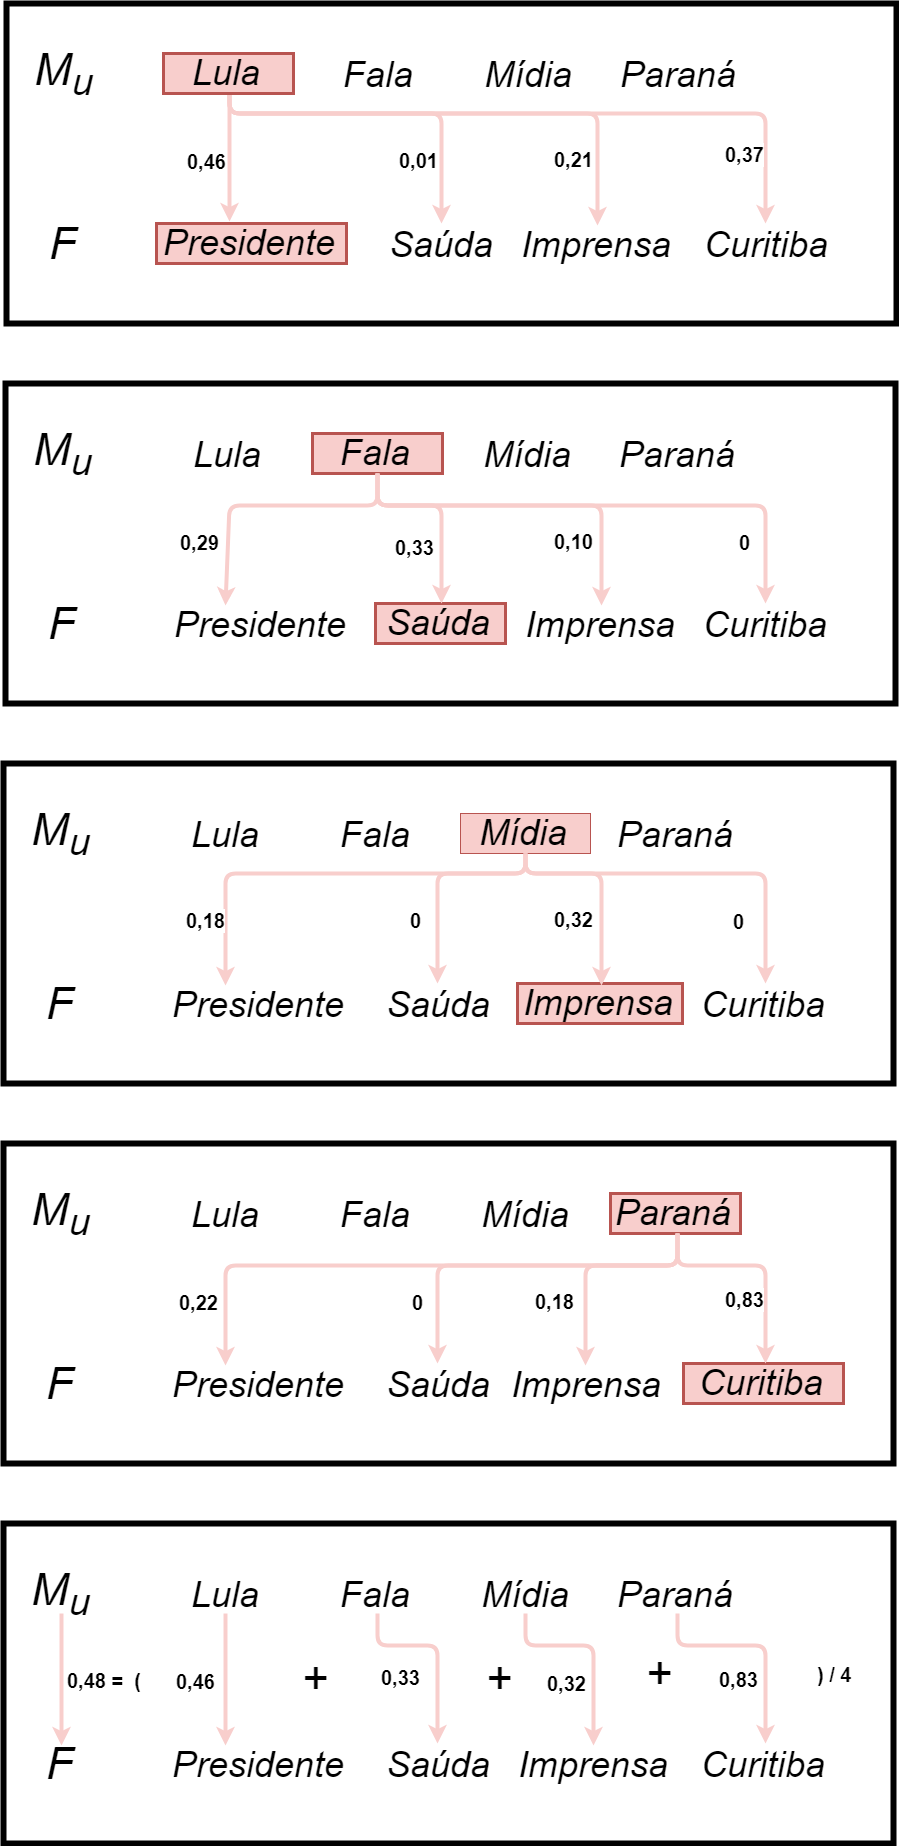
\includegraphics[scale=0.32]{imagens/rlws_ex.png}
	\caption{Imagem que exemplifica o fluxo da recomendação.}
	\label{fig:rlws_ex}
\end{figure}

\section{Estrutura de Cache para Recomendação}
\label{sec:cache}

É importante ressaltar que para este projeto foi desenvolvido um sistema de \textit{cache} para o cálculo da similaridade de recomendação dos filmes, dividido-se em duas camadas:

\begin{itemize}
	\item{\textbf{Cache remoto com banco de dados}: Para calcular a similaridade entre dois tokens quaisquer, o sistema utiliza uma Equação (\ref{eq:rlws}) de similaridade que tira proveito do serviço da DBPedia. Na equação, conforme abordado em \ref{ssec:sim_rec} realiza-se a contagem de links diretos e indiretos dos recursos. Essa contagem posteriormente é armazenada no banco de dados para uma consulta mais ágil.}
	\item{\textbf{Cache local, em memória}: A cada comparação realizada é verificado inicialmente se a mesma está presente no cache remoto, evitando consultas desnecessárias ao DBPedia. Após a verificação, a comparação é armazenada num cache local em memória de execução (\ac{RAM}). O objetivo é que durante o cálculo da recomendação de um usuário não seja necessário realizar a todo instante consultas ao banco, visto o volume de comparações, já que cada palavra dos termos do usuário é comparada com todas as palavras dos filmes. O processo de realizar tais consultas ao banco no momento da comparação prejudica o desempenho da aplicação. Assim, optou-se por utilizar a estrutura de \textit{cache} em memória fornecida pelo \textit{framework} Spring\footnote{https://spring.io}. Após um determinado número de comparações o sistema verifica quais delas precisam ser persistidas, salvando-as em sequência e posteriormente liberando o cache em memória.}
\end{itemize}

Com esse sistema minimiza-se o tráfego de dados entre a aplicação, o DBPedia e o banco de dados durante a comparação de filmes, acelerando o processo, além de ter um bom balanço de desempenho entre o cache remoto e cache local

\section{Tecnologias}

Para o desenvolvimento do sistema foram escolhidas algumas tecnologias para arquitetura software, como linguagens de programação, \textit{framework} \ac{MVC}, processamento e banco dados, entre outras. A seguir serão apresentadas as tecnologias utilizadas.

\subsection{JAVA}

JAVA\footnote{https://www.java.com} é uma linguagem de programação de propósito genérico, desenvolvida originalmente por James Gosling na Sun Microsystems\footnote{ https://www.oracle.com/br/sun/index.html} em 1995. Atualmente a linguagem foi comprada pela Oracle Corporation\footnote{https://www.oracle.com}. As características em destaque da linguagem estão no fato de ser baseada em classes e orientada a objetos. A \ac{OOP} é um paradigma de programação que abstrai conceitos em objetos, que podem conter dados, campos e comportamentos nomeados de \textit{methods} \citep{Lewis2000}.

Outra caraterística importante da linguagem trata-se da filosofia apresentada pelos desenvolvedores de “escreva uma vez, rode em qualquer lugar”. A filosofia trata-se da linguagem ser compilada por uma \ac{VM} possibilitando escrever um mesmo pedaço de código que possa ser portado para outra plataforma sem necessidade de alterá-lo, uma vez que cada \ac{VM} implementa as especificidades da nova plataforma abstraindo o acesso ao \ac{SO}.

A linguagem JAVA é usada em diversos sistemas e plataformas, com inúmeros propósitos, desde aplicações \textit{desktop}, pesquisa científica, desenvolvimento Web entre outros propósitos.

\subsection{Spring Boot}

Spring Boot\footnote{https://projects.spring.io/spring-boot/} é um projeto da Pivotal Software\footnote{https://pivotal.io} para facilitar o processo de configuração e publicação de aplicações e serviços providos pelo Spring\footnote{https://spring.io}, com baixo esforço e configuração. O \textit{Spring} é um framework \textit{open source}\footnote{Modelo de desenvolvimento que promove um licenciamento livre para o design ou esquematização de um produto} que provê um compreensivo conjunto de modelos de configuração para aplicações JAVA. O elemento principal do \textit{Spring} é prover infraestrutura para aplicações oferecendo os seguintes principais recursos:

\begin{itemize}
	\item{\textbf{Inversão de Controle}: \ac{IOC}, também conhecido como \textit{dependency injection} é um princípio em que as “dependências” devem ser supridas, injetadas por outro objeto. As dependências são objetos que serão usados como “serviços” para acessar suas funcionalidades, dentro dos \textit{containers} de \ac{IOC}. A injeção é a passagem da dependência para um objeto (o cliente) \citep{DependencyInjection2006}. O termo “inversão de controle” origina-se do fato que a criação de valores de classes externas ao objeto não deve ser realizada pelo próprio objeto mas, sim pelos \textit{containers} de \ac{IOC}.}

	\item{\textbf{Acesso a dados}: O framework possui diversas bibliotecas para o acesso a dados, tanto para bancos relacionais como não relacionais. Também é oferecido um sistema \ac{ORM} que trata-se de uma técnica para traduzir o formato de dados de um banco relacional para \ac{OOP}, facilitando sua manipulação.}

	\item{\textbf{Arquitetura MVC}: Fornece todo suporte para customizar e criar uma arquitetura \ac{MVC}.}
\end{itemize}

\subsection{HTML, CSS, Javascript}

O HTML\footnote{https://www.w3.org/html}, \ac{CSS}\footnote{https://www.w3.org/Style/CSS/} e JavaScript forma a principal pilha de tecnologias utilizadas na Web. O HTML é uma linguagem de marcação mantida pela \ac{W3C} para criação de páginas, originalmente desenvolvida por Tim-Berners-Lee \citep{Raggett1998}. O objetivo é a fácil construção e publicação de conteúdo no ambiente Web e consequentemente na \ac{WWW}. No \textit{Spring Boot} as páginas HTML podem ser escritas utilizando algum dos mecanismos de \textit{templates}, como o \textit{thymeleaf}. Uma das vantagens da utilização desses mecanismos é a herança de visualizações, assim como facilidade de interligar em manipular os dados passados pela camada do \textit{controller} no \ac{MVC}.

O \ac{CSS} é uma linguagem para criar regras de estilização das páginas \ac{HTML}. O CSS cria ou altera um formato de apresentação (tamanho, cores, margens etc) de algum elemento do HTML, como blocos, parágrafos, imagens entre outros. Quanto ao JavaScript é uma linguagem de programação originalmente criada por Brendan Eich na Netscape Communications\footnote{ http://isp.netscape.com}. A linguagem é utilizada para controlar o comportamento de páginas HTML, oferecendo dinamicidade, podendo alterar elementos da página em tempo real.

\subsection{MySQL}

O MySQL\footnote{https://www.mysql.com} trata-se de um \ac{SGBD} que utiliza a linguagem \ac{SQL} para manipulação de dados guardados em um sistema de arquivos \citep{MySQLSGBD}. Originalmente desenvolvido por Michael Widenius em 1994, o seu foco é para o desenvolvimento de aplicações Web, embora tenha se popularizado para a maioria das plataformas existentes \citep{MySQLDevelopers}. Foi o banco de dados escolhido para a persistência de dados da aplicação, além de ser de fácil integração com o \textit{framework} \textit{Spring Boot}.

\subsection{Apache Jena}

Apache Jena\footnote{https://jena.apache.org} é um \textit{framework} \textit{open source} para Web Semântica, escrito na linguagem Java. A biblioteca provê uma \ac{API} que facilita a extração e criação de dados nos grafos do \ac{RDF}, além de oferecer suporte para a linguagem de consulta \ac{SPARQL}. O objetivo da escolha dessa tecnologia para o projeto, é para facilitar a busca e navegação pelo grafo de entidades (\textit{resources}) no sistema da DBPedia\footnote{http://wiki.dbpedia.org} utilizando \ac{SPARQL}. Após o \ac{SR} extrair entidades das descrições do filme, essas serão buscadas no serviço da Web Semântica estendendo o conhecimento do recurso.

\subsection{Apache OpenNLP}
\label{ssec:open_nlp}

Apache OpenNLP\footnote{https://opennlp.apache.org} é um \textit{framework} \textit{open source} de aprendizado de máquina que é usado para processamento de \ac{NLP}. A biblioteca provê uma \ac{API} com serviços para geração de \textit{tokens}, sentenças, segmentação, reconhecimento de partes da fala, extração de entidade de nome, geração de \textit{chunks} (pedaços), entre outras tarefas do \ac{NLP}.

No projeto essa tecnologia será utilizada para o \ac{NER} e extração de partes gramaticais presentes na descrição do filme, assim como a geração dos \textit{tokens}. O objetivo é que com essa biblioteca seja possível gerar \textit{tokens} com entidades encontradas, de nomes localizações, como também partes do texto de nomes próprios, substantivos e adjetivos.

\subsection{Apache Lucene}

Apache Lucene\footnote{https://lucene.apache.org} é um \textit{framework} \textit{open source} para sistemas de recuperação de informação e recomendação. O projeto oferece dois principais recursos: indexação e pesquisa de texto. Lucene é muito reconhecido por sua utilidade na implementação em mecanismos de buscas na Internet \citep{McCandless2010}. O projeto também é muito utilizado em sistemas de recomendação com implementação de diversos algoritmos para calcular a similaridade de documentos.
No projeto essa tecnologia será utilizada para tirar proveito dos algoritmos de similaridade, como o \textit{cossine similarity} (ver \ref{eq:cosine_sim}), possibilitando realizar comparações com as métricas propostas no trabalho.

\section{Sumário}

Neste capítulo foram apresentadas as funcionalidades para a proposta do sistema de recomendação, assim como as tecnologias empregadas. Também foram abordadas as etapas do ciclo de vida da aplicação, demonstrando o modelo de dados, assim como a etapa de preparação para recomendação. Por fim foi elaborada a proposta de um novo método de similaridade semântica, mostrando suas características e equações, além dos algoritmos para geração das recomendações. No próximo capítulo serão apresentados os resultados obtidos com novo método elaborado, junto técnicas para sua obtenção, assim como a comparação com outros modelos.

\chapter{Avaliação}
\label{cap:evaluation}

Neste capítulo serão apresentadas as avaliações da solução proposta, metodologias utilizadas, conjunto de dados estudados, métricas e discussões sobre o significado dos resultados em relação aos objetivos inicialmente traçados. Espera-se que com o desenvolvimento de uma métrica de similaridade semântica, explorando as relações de recursos no DBPedia\footnote{http://wiki.dbpedia.org}, seja possível tirar vantagem para sugerir itens, invés da análise mais sintática do conteúdo utilizado em métodos como \ac{TFIDF}. Também é desejado verificar o impacto do uso da sinopse do filme, um dado não estruturado, invés de itens mais comuns como gênero, diretor, atores, com o objetivo de \enquote{fugir} das recomendações que prendam mais o usuário no mesmo tipo de filmes, mas ainda assim ser capaz de ser relevante aos seus interesses.

Inicialmente serão apresentados os dados utilizados e resultados iniciais do uso da métrica de similaridade utilizada, analisando os efeitos desejados. Posteriormente o método de recomendação que utiliza a similaridade semântica apresentado na seção \ref{ssec:formula_rlws} será comparado com o método da similaridade do cosseno, utilizando-se métricas que serão definidas e apresentadas. O resultado esperado é de que utilizando um método que leve em consideração relações semânticas tenha melhores resultados daqueles que apenas possuem análises sintáticas. Por fim, serão abordadas discussões sobre resultados alcançados além de pontos de melhoria.

\section{Metodologia}
\label{sec:methodology}

Na avaliação de um sistema de recomendação é importante entender sua eficácia e seus algoritmos envolvidos, uma vez que uma análise incorreta pode levar subestimação ou superestimação da sua real precisão, como aponta \cite{Aggarwal2016:Evaluation}. Sendo assim, recomendadores podem ser avaliados tanto usando métodos denominados como \textit{online} ou \textit{offline}. Num sistema \textit{online} as opiniões e reações dos usuários são consideradas e medidas de acordo com as recomendações apresentadas, tendo sua participação de fato, como algo crucial para a compreensão dos resultados. Contudo, como a avaliação desse método requer a participação do usuário, o que nem sempre é viável, também existe o método \textit{offline}, onde um conjunto de diferentes tipos de dados históricos dos usuários são utilizados \citep{Herlocker:1999}. Para os experimentos descritos nesta seção, serão utilizados em sua maioria um conjunto de dados offline retirados do projeto MovieLens\footnote{https://movielens.org}, conforme apresentado na seção \ref{sec:av_data_set}. Utilizando-se da mesma metodologia também serão avaliados resultados de testes online, mas para um grupo bem pequeno, apenas para realizar uma comparação da diferença de resultados encontrados.

O objetivo dos experimentos que serão apresentados, é avaliar se a utilização da similaridade semântica junto ao método de recomendação proposto, é capaz de trazer resultados melhores nas métricas de avaliação em relação a similaridade do cosseno utilizando \ac{TFIDF}.  Os resultados tratam-se das análises das métricas extraídas das avaliações realizadas por usuários em relação as recomendações geradas por esses métodos.

Para realizar os testes entre os dois métodos de recomendação é necessário construir um perfil do usuário,
formado através dos filmes que avaliou. Cada usuário deve ter pelo menos 10 avaliações. Com intuito de captar os interesses do usuário, definiu-se que para montar o modelo do usuário com seus melhores termos, serão utilizados apenas os filmes com avaliação igual ou superior a 3,5, sendo 5 a avaliação máxima. No capítulo \ref{cap:proposal} foi definido que o perfil do usuário seria um conjunto $M_u$ dos melhores termos, possuindo um tamanho $z$ constante. Nos experimentos a seguir foi estipulado $z$ como 15 termos. A quantidade de termos definida possui um impacto grande na performance do sistema, uma vez que a complexidade do algoritmo da comparação entre termos é de $O(zm)$ (considerando $z$ como constante tem-se $O(m)$), sendo $m$ a quantidade de termos do filme. A Figura \ref{fig:tempo_x_termos} demonstra um gráfico da quantidade de termos do modelo do usuário em relação ao tempo de processamento, considerando que todos os dados estão no \textit{cache local}, conforme abordado no capítulo \ref{cap:proposal}, ou seja, o melhor caso.

\begin{figure}
	\centering
	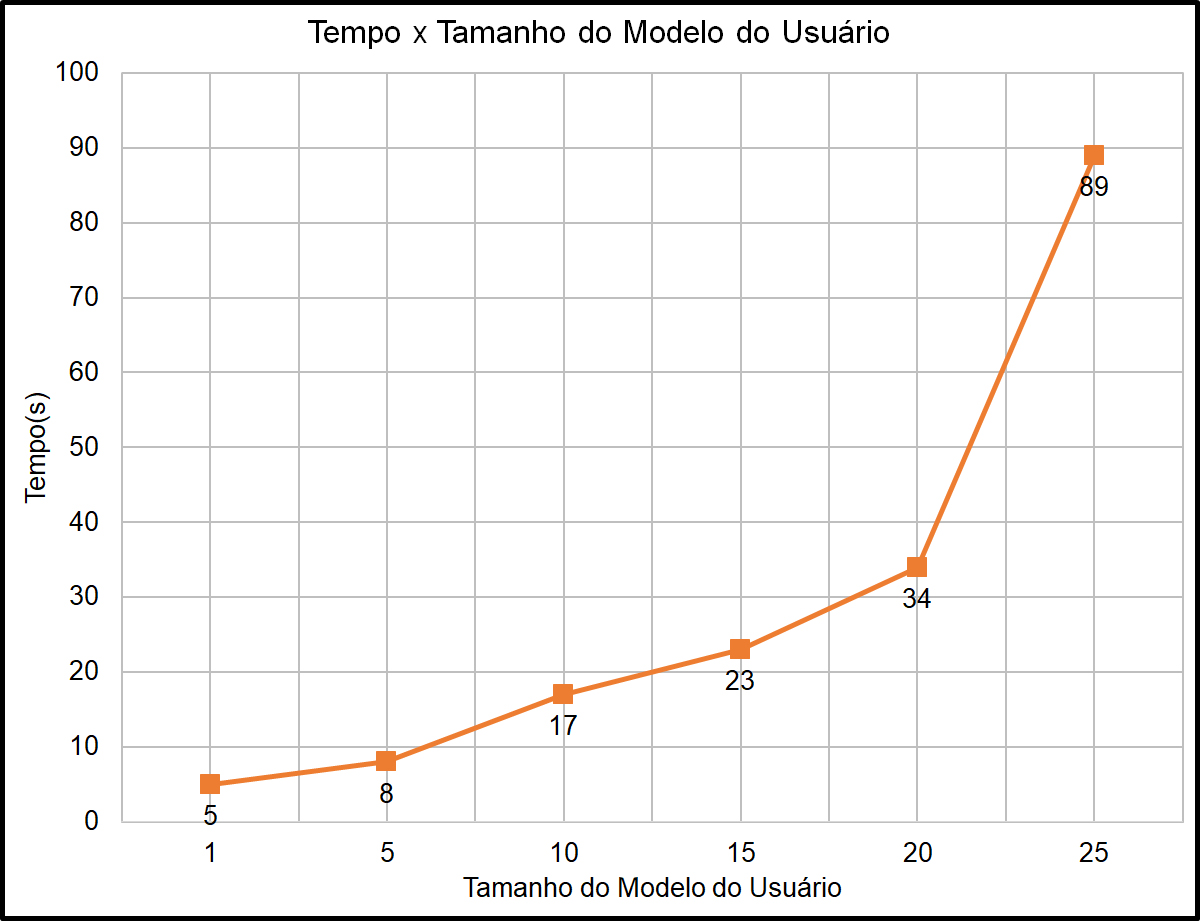
\includegraphics[scale=0.3]{imagens/tempo_x_termos.jpg}
	\caption{Gráfico da relação do tamanho do modelo do usuário (quantidade de termos usados) com o tempo de processamento para recomendação de um usuário. Todas as comparações de termos estão em \textit{cache}. Execução numa máquina com processador \textit{i7 6700K}, 16GB RAM, \textit{Windows 10}.}
	\label{fig:tempo_x_termos}
\end{figure}

Definida a metodologia para a construção do perfil do usuário, na análise dos resultados serão realizados 3 experimentos para construir as recomendações. O total de recomendações possíveis trata-se de todos os outros filmes que o usuário não avaliou, o que torna extremamente trabalhosa a sua avaliação, portando indo contrário aos propósitos de um \ac{SR}, como filtrar e classificar resultados personalizados, poupando-o tempo na busca por informações. Sendo assim, apenas uma quantidade pequena de filmes serão recomendados, sendo um total de 20 recomendações com melhores scores, por experimento, uma vez que o importante é avaliar os bons primeiros resultados, ou aqueles exibidos primeiramente, pois conforme cada vez o usuário tem que continuar procurando por resultados, pior pode ser a percepção de relevância, conforme argumentado por \cite{Manning:2008}. 

Os três experimentos consistem nas seguintes abordagens:

\begin{enumerate}
	\item{\textbf{Experimento 1}: Serão construídas recomendações utilizando o método apresentado na seção \ref{ssec:formula_rlws}, definindo os pesos como 0,8 para links diretos e 0,2 para indiretos. A seguir este experimento será referido como \textbf{RLWS DIRECT}, indicando que a prioridade nos relacionamentos diretos entre recursos.}
	\item{\textbf{Experimento 2}: Semelhante ao experimento 1, mas com pesos 0,2 para links diretos e 0,8 para indiretos. Este experimento será referido como \textbf{RLWS INDIRECT} para indicar a prioridade dos relacionamentos indiretos entre recursos.}
	\item{\textbf{Experimento 3}: Recomendações construídas utilizando o método da similaridade do cosseno, referenciada por \textbf{COSINE}.}
\end{enumerate}

O objetivo da variação dos pesos para a similaridade \ac{RLWS} é analisar o comportamento privilegiando o relacionamento direto ou indireto de recursos na DBPedia.
 
É importante ressaltar que para os testes \textit{online}, os usuários serão entrevistados, fornecendo um conjunto de 10 filmes de sua preferência, além de que não será detalhado qual método foi utilizado para as recomendações geradas por cada experimento. Para cada item recomendado o usuário terá de avaliar com uma nota de 0 a 5 estrelas, onde serão considerados os itens relevantes como aqueles que possuírem 3,5 estrelas ou mais. Já para os testes offline, como não há como saber a avaliação do usuário, será utilizada uma média das avaliações de outros usuários, onde também serão consideradas relevantes aquelas avaliações com média superior ou igual a 3,5 estrelas.

Para medir os resultados das recomendações dos experimentos serão utilizadas métricas como \textit{Precision} e \textit{Recall}, que dependem de um modelo de classificação binária \citep{Powers_2008}, sendo assim avaliações maiores ou iguais a 3,5 estrelas serão consideradas relevantes ou positivas, e inferiores como irrelevantes ou negativas. Na seção \ref{sec:av_metrics} serão melhor discutidas as métricas empregadas para avaliar os experimentos, assim como seus resultados.

Na seção seguinte será apresentado os dados trabalhados e gerados durante a execução dos experimentos.

\section{Conjunto de dados}
\label{sec:av_data_set}

Os dados usados durante os experimentos tratam-se de filmes , usuários com seus termos extraídos pelo processo do \ac{NLP}, além de avaliações. A Tabela \ref{tab:dataset} demonstra a quantidade de dados utilizados durante os testes. Note que os \enquote{URIs válidas} tratam-se termos extraídos das sinopses que possuem uma \ac{URI} associada a um recurso no DBPedia\footnote{http://wiki.dbpedia.org}. Os \enquote{usuários, teste offline} e \enquote{online} tratam-se da quantidade de usuários utilizados do total, em que foram geradas as recomendações dos experimentos.

\begin{table}[H]
\centering
\def\arraystretch{1.3}
\begin{tabular}{|l|l|}
	\hline
	\textbf{Dado}          & \textbf{Quantidades}   \\ \hline
	Filmes                 & 5.107                  \\ \hline
	Usuários               & 100.004                \\ \hline
	Usuários, teste offline & 30					\\ \hline
	Usuários, teste online & 4						\\ \hline
	Total de avaliações       & 11.997.970          \\ \hline
	Total URIs             & 22.978                 \\ \hline
	Total URIs válidas     & 18.630                 \\ \hline
	Total de comparações de URIs & 6.306.451        \\ \hline
\end{tabular}
\caption{Contagem dos dados utilizados durante os testes.}
\label{tab:dataset}
\end{table}

O total de URIs válidas é um ponto de contenção importante de ser analisado, uma vez que se o termo não se trata de um recurso na DBPedia, a comparação do \ac{RLWS} é descartada. Sendo assim, algo importante para a viabilidade da similaridade é de que a maioria dos termos extraídos das descrições dos filmes, tenha uma \ac{URI} associada ao recurso. A Tabela \ref{tab:lod_statistics} demonstra algumas estatísticas em relação aos termos extraídos dos filmes. Abaixo é descrito os conceitos construídos para a análise dos dados da tabela.

\begin{itemize}
	\item{\textbf{Cobertura DBPedia}: Trata-se do percentual dos termos encontrados que possuem uma \ac{URI} associada no DBPedia. É importante que este valor seja alto, pois caso não sejam encontrados os termos no serviço da web semântica a similaridade torna-se inválida.}
	
	\item{\textbf{Cobertura Links Diretos}: É o percentual de links que possuem pelo menos um relacionamento direto com outro termo dentro do conjunto de dados do experimento. Este valor revela o quão útil pode ser comparar dois termos quaisquer buscando por relacionamentos diretos no DBPedia, conforme abordado no capítulo \ref{cap:proposal}.}
	
	\item{\textbf{Cobertura Links Indiretos}: Similar à cobertura de links indiretos, mas agora sendo o percentual de links que possuem pelo menos um relacionamento indireto com outro termo.}
	
	\item{\textbf{Cobertura de Filmes com Links Diretos}: É o percentual de filmes contendo pelo menos um termo com ao menos um relacionamento direto a outro termo. Este valor tem o intuito de demonstrar a viabilidade da comparação utilizando a métrica \ac{RLWS} para comparar filmes utilizando-se os termos extraídos das suas descrições. A ideia é de que a maioria dos filmes possam utilizar a comparação de termos, tendo pelo menos um termo com relacionamento a outro encontrado.}
	
	\item{\textbf{Cobertura de Filmes com Links Indiretos}: O mesmo da cobertura de filmes com links diretos, mas agora sendo o percentual para os indiretos.}
\end{itemize}

\begin{table}[H]
\centering
\begin{tabular}{|l|l|}
\hline
\textbf{Dado}                           & \textbf{Valor} \\ \hline
Cobertura DBPedia                       & 81,08\%        \\ \hline
Cobertura Links Diretos                 & 21,63\%        \\ \hline
Cobertura Links Indiretos               & 64,41\%        \\ \hline
Cobertura de Filmes com Links Diretos   & 99,96\%        \\ \hline
Cobertura de Filmes com Links Indiretos & 100,00\%       \\ \hline
\end{tabular}
\caption{Estatística da cobertura dos dados dos links de recursos na DBPedia}
\label{tab:lod_statistics}
\end{table}

É importante ressaltar que os dados das coberturas apenas consideram os \enquote{links válidos}, ou seja, aqueles que possuem uma URI associada no DBPedia. Nota-se também que os dados mencionados na tabela em relação a cobertura de links diretos e indiretos trata-se das comparações realizadas nos experimentos, sendo assim, não se completam, pois ainda existem links com relacionamentos que não foram comparados.

Algo relevante para destacar quanto à relação entre recursos é de que a quantidade de relacionamentos entre recursos cujo a quantidade links diretos é maior que 0, é de aproximadamente 0,12\% em relação ao total de relações entre recursos, conforme constatado na Tabela \ref{tab:lod_cache_stats}. Já era esperado que a maioria dos recursos não tivesse propriedades diretamente conectadas entre si, devido a variedade de comparações indiscriminada entre termos do usuário e termos dos filmes. Isso resulta numa tabela de dados altamente esparsa em relação ao cálculo a participação direta na equação \ac{RLWS}, o que por consequência leva a uma tabela de dados grande contendo diversas comparações zeradas. Quanto a proporção de relacionamentos indiretos maiores que 0 em relação ao total é de aproximadamente 8,05\%. Embora esses valores sejam baixos, o foco é de que para cada termo existam pelo menos um relacionamento a outro termo, seja direta ou indiretamente, e de que esse relacionamento esteja distribuído pela maioria dos filmes, algo que é evidenciado pelos dados da Tabela \ref{tab:lod_statistics}. Na tabela abaixo ainda são apresentados os de recursos relacionados que possuem a propriedade \textit{dbo:wikiPageRedirects}, ou seja, aqueles que o DBPedia resolve sua \ac{URI} como sendo a mesma, portanto para a similaridade considerados iguais.

\begin{table}[H]
\centering
\def\arraystretch{1.3}
\begin{tabular}{|l|l|}
\hline
\textbf{Dado}                                   & \textbf{Quantidades} \\ \hline
Relação entre recursos                          & 6.306.451            \\ \hline
Relação entre recursos, direto $> 0$ 			& 7.977                \\ \hline
Relação entre recursos, indireto $> 0$ 			& 510.533              \\ \hline
Relação entre recursos, redirecionados entre si & 194                  \\ \hline
Relação entre recursos, direto e indireto $= 0$ & 5.794.914            \\ \hline
\end{tabular}
\caption{Contagem da relação entre recursos utilizados durante os experimentos.}
\label{tab:lod_cache_stats}
\end{table}

\section{Métricas de avaliação}
\label{sec:av_metrics}

Existem diversas métricas que são usadas tanto em avaliações \textit{online} e \textit{offline}, mas as mais comuns são as de \textit{accuracy}, embora existam outras como \textit{user coverage}, \textit{novelty}, \textit{trust} \citep{Jannach:2010}. Para este trabalho foram utilizadas tanto avaliações \textit{online} e \textit{offline}, com métodos de precisão para avaliar as classificações da recomendações, como \textit{Precision} e \textit{Recall}. Abaixo serão abordados os conceitos das métricas de avaliação utilizadas nos experimentos.

\subsection{Precision}

Avaliando recomendações com métodos \textit{offline} apenas utilizando dados históricos da preferência do usuário, somente pode informar aqueles itens que foram de conhecimento do usuário, portando todos os outros itens terão de avaliados de outras formas, que não seja diretamente pela sua opinião, o que pode levar à falso positivos e/ou negativos. Por outro lado, avaliando com usuários reais, esses podem julgar todos os itens recomendados, podendo de fato definir se a predição foi correta ou não. Com a avaliação do usuário é possível construir uma tabela de classificação conforme a Figura \ref{fig:truth_table} \citep{Jannach:2010}, onde há o cruzamento entre o que o recomendador apresentou e o que usuário avaliou. Se um item foi apresentado na recomendação e o usuário tenha gostado, avaliado como relevante, tem-se um caso de predição correta, ou \textit{true positive}. Outro resultado positivo, trata-se de quando o usuário não tenha gostado e o recomendador omitiu o resultado, ou seja uma omissão correta ou \textit{true negative}. Assim os resultados positivos estão na diagonal da esquerda para direita da tabela, e os resultados não desejados e negativos estão na outra diagonal. 

\begin{figure}
	\centering
	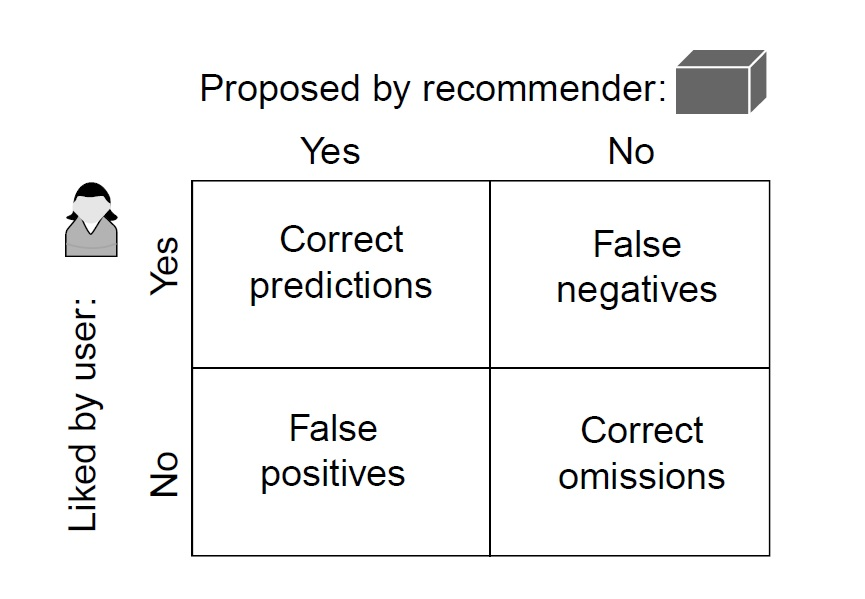
\includegraphics[scale=0.4]{imagens/truth_table.jpg}
	\caption{Tabela de tipos de erros baseada na ilustração de \cite{Jannach:2010}.}
	\label{fig:truth_table}
\end{figure}

Considerando e classificando os resultados dessa forma binária, em positivos e negativos, defini-se \textit{precision}, precisão ou confiança, como sendo a fração de resultados previstos e avaliados pelo usuário como positivos, ou seja, os \textit{true positive}, em relação a quantidade de todos os itens recomendados \citep{Powers_2008}. A Equação \ref{eq:precision} demonstra o cálculo da precisão $P$, onde $tp$ trata-se da quantidade de itens \textit{true positive} e $fp$ como \textit{false positive}.

\begin{equation}
	P = \frac{tp}{tp + fp}
\label{eq:precision}
\end{equation}

Como a quantidade de resultados pode ser muito grande para calcular a precisão, e até para que o próprio usuário o faça, por extensão também defini-se como $P@k$, como sendo a precisão até $k$ primeiros resultados retornados pelo recomendador \citep{Aggarwal2016:Evaluation}. A Equação \ref{eq:precision_at_k} demonstra a variação do cálculo de $P$ onde $r$ trata-se da quantidade de itens relevantes até o \textit{rank} $k$. \ref{eq:precision_at_k}.

\begin{equation}
	p@k = \frac{r}{k}
\label{eq:precision_at_k}
\end{equation}

\subsection{Mean Average Precision (MAP)}

Outra métrica de precisão trata-se da \ac{MAP}, que busca estipular um único valor de precisão em relação ao conjunto de avaliações de múltiplos usuários \citep{Manning:2008}. A equação \ref{eq:map} demonstra o cálculo, onde $AveP(u)$ trata-se da média das precisões $p@k$ do usuário $u \in U$, onde $|R|$ é quantidade de itens relevantes até $k$-ésimo \textit{rank}. Posteriormente obtém-se o $MAP$ como sendo a média $AveP$ para todos os usuários avaliados. A Figura \ref{fig:map_ex} exemplifica o cálculo da métrica, onde os quadrados \enquote{verdes} representam os itens \textit{true positive} e os itens vermelhos os \textit{false positive}.

\begin{equation}
	AveP(u) = \frac{\sum_{k=1}^{n} p@k}{|R|}, \; u \in U
\label{eq:avep}
\end{equation}

\begin{equation}
	MAP = \frac{\sum_{u=1}^{|U|}AveP(u)}{|U|}
\label{eq:map}
\end{equation}

\begin{figure}
	\centering
	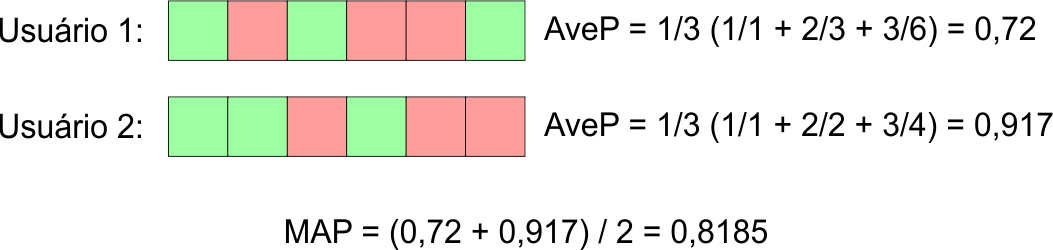
\includegraphics[scale=0.4]{imagens/map_ex.jpg}
	\caption{Exemplo do cálculo do MAP.}
	\label{fig:map_ex}
\end{figure}

\subsection{Mean Reciprocal Rank (MRR)}

A métrica \ac{MRR} trata-se da média da classificação recíproca (\textit{reciprocal rank}) de cada usuário \citep{Burges:2006}, sendo esta o multiplicativo inverso a posição do primeiro item correto no \textit{rank} de recomendações, ou top-N itens. O objetivo é obter um valor geral que informe o quão longe o primeiro resultado positivo está do primeiro item. A Equação \ref{eq:mrr} demonstra o cálculo onde $\frac{1}{k}$ trata-se do \textit{reciprocal rank} até o $k$-ésimo item. A Figura \ref{fig:mrr_ex} exemplifica o cálculo da métrica, onde os quadrados \enquote{verdes} representam os itens \textit{true positive} e os itens vermelhos os \textit{false positive}.

\begin{equation}
	MRR = \frac{1}{|U|} \sum_{u=1}^{|U|} \frac{1}{k}, \; u \in U
\label{eq:mrr}
\end{equation}

\begin{figure}
	\centering
	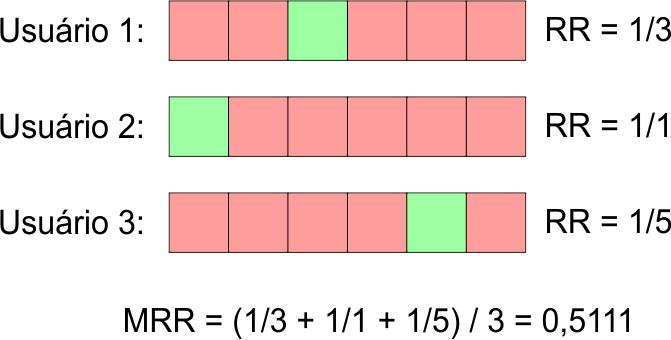
\includegraphics[scale=0.4]{imagens/mrr_ex.jpg}
	\caption{Exemplo do cálculo do MRR.}
	\label{fig:mrr_ex}
\end{figure}

\section{Resultados}
\label{sec:results}

Antes de apresentar os resultados das recomendações com as avaliações dos usuários, é importante avaliar algumas premissas e comportamentos da própria equação de similaridade, a \ac{RLWS}. Inicialmente o esperado é de que recursos que sejam intuitivamente próximos, ou provavelmente tenham diversas relações entre si,  como \textit{Earth} e \textit{Moon}, possuam maior similaridade do que \textit{Earth} e \textit{Table}. E de fato, mesmo nos dois extremos de pesos, seja priorizando as links diretos ou indiretos, existe uma diferença considerável quando termos estão intuitivamente mais próximos do que aqueles que provavelmente não terão relacionamentos em comum, conforme mostra Figura \ref{tab:rlws_results}. É importante ressaltar que \enquote{RLWS DIRECT} refere-se à configuração de pesos $w_d = 0,8, w_i = 0,2$, enquanto que \enquote{RLWS INDIRECT} é o inverso, assim priorizando os relacionamentos indiretos entre dos termos.

\begin{table}[H]
\centering
\begin{tabular}{|l|l|l|l|}
\hline
\textbf{Termo 1} & \textbf{Termo 2}    & \textbf{RLWS DIRECT} & \textbf{RLWS INDIRECT} \\ \hline
France           & Paris               & 0,434                   & 0,858                   \\ \hline
France           & Juice               & 0,111                   & 0,443                   \\ \hline
France           & Art                 & 0,190                   & 0,760                   \\ \hline
Brazil           & Brasilia            & 0,193                   & 0,770                   \\ \hline
Brazil           & Box                 & 0,050                   & 0,200                   \\ \hline
Brazil           & Paper               & 0,163                   & 0,652                   \\ \hline
Brazil           & Beach               & 0,282                   & 0,726                   \\ \hline
Car              & Automobile          & 1,0                     & 1,0                     \\ \hline
United\_States   & Washington,\_D,C,   & 0,372                   & 0,842                   \\ \hline
China            & Hong\_Kong          & 0,377                   & 0,842                   \\ \hline
Ariana\_Grande   & Selena\_Gomez       & 0,320                   & 0,800                   \\ \hline
Selena\_Gomez    & Elon\_Musk          & 0,022                   & 0,087                   \\ \hline
Coconut          & Plant               & 0,393                   & 0,683                   \\ \hline
Tom\_Cruise      & Lady\_Gaga          & 0,162                   & 0,646                   \\ \hline
Star             & Galaxy              & 0,339                   & 0,809                   \\ \hline
Earth            & Moon                & 0,485                   & 0,866                   \\ \hline
Earth            & Table               & 0,033                   & 0,132                   \\ \hline
Book             & Movie               & 0,125                   & 0,500                   \\ \hline
Book             & Metal               & 0,096                   & 0,386                   \\ \hline
Johnny\_Cash     & June\_Carter\_Cash  & 0,579                   & 0,868                   \\ \hline
Johnny\_Cash     & Al\_Green           & 0,176                   & 0,705                   \\ \hline
Johnny\_Cash     & Elvis\_Presley      & 0,316                   & 0,816                   \\ \hline
Johnny\_Cash     & Kris\_Kristofferson & 0,317                   & 0,804                   \\ \hline
Johnny\_Cash     & Carlene\_Carter     & 0,457                   & 0,743                   \\ \hline
\end{tabular}
\caption{Tabela de amostra de comparações entre termos usando \ac{RLWS}.}
\label{tab:rlws_results}
\end{table}

É importante ressaltar que mesmo para termos que estejam aparentemente mais distantes, como \textit{Selena\_Gomez} e \textit{Ariana\_Grande}, por se tratarem de "coisas" que não são imediatamente próximas, ainda possuem uma alta similaridade, devido as conexões que ambas as pessoas possuem quanto ao domínio da música e aparições em temas de filmes, programas etc. Já quando compara-se \textit{Selena\_Gomez} com \textit{Elon\_Musk}, mesmo também sendo uma comparação entre pessoas, já possuem uma similaridade bem menor, o que também é intuitivamente esperado. Também se observa na comparação \textit{Johnny\_Cash} e \textit{June\_Carter\_Cash}, uma alta similaridade, pois os dois foram casados e cantores. Outra observação importante é quanto aos termos \textit{Car} e \textit{Automobile} que possuem similaridade 1. Isso é devido que os dois possuem a propriedade \textit{dbo:wikiPageRedirect} conectando seus recursos, o que por regra na equação terá valor 1. Esses redirecionamentos também ocorrem nos termos \textit{Future} e \textit{Futuristic}, \textit{Power} e \textit{Powerful} entre outros. Para uma série de termos esses redirecionamentos contribuem para o desempenho da equação, devido a sua real proximidade, apesar de serem termos diferentes.

Nota-se que intuitivamente os resultados das comparações fazem sentido tanto usando pesos que privilegiam links diretos ou indiretos, o que é vital para coerência no momento da comparação termo a termo. Outro fato importante é a consideração de itens que possuem redirecionamentos, ainda que sejam raros, mas para palavras como "Carro" e "Automóvel" é sensato dizer que são similares.

Avaliadas as premissas e os resultados para a similaridade semântica proposta, em sequência serão calculados as métricas mencionadas na seção \ref{sec:av_metrics}, medindo assim o impacto do modelo de recomendação assim como a própria similaridade \ac{RLWS}. Os testes dos experimentos mencionados na seção \ref{sec:methodology} serão divididos em dois resultados, os testes com dados de \enquote{usuários offline} e \enquote{usuários offline}.

\subsection{MAP}

Para medir a assertividade do \ac{SR} foi utilizada a métrica \ac{MAP} perante dois conjuntos de usuários, os dos testes \textit{offline} (sendo no total de 30) e os \textit{online} (com total de 4). As Figuras \ref{fig:map_line} e \ref{fig:map_box_plot} apresentam os resultados obtidos nos três experimentos, tanto para os testes online quanto para os offline. 

O mais notável dos valores obtidos é o fato de que os testes do experimento 2, com \textit{RLWS INDIRECT}, teve um desempenho consideravelmente melhor que os outros nos dois testes, em especial a seu par que privilegia os links diretos, sendo 51\% superior (0,532 contra 0,351) ao \textit{COSINE} para $p@5$ nos testes \textit{offline}. Quanto aos resultados utilizando a métrica \textit{RLWS DIRECT}, há uma divergência entre os testes das Figuras \ref{fig:map_line_a} e \ref{fig:map_line_b}, sendo que o primeiro teste obteve um desempenho próximo à métrica \textit{COSINE}, na verdade até perdendo, enquanto que nos testes \textit{offline} ganha em 27\% (0,447 contra 0,351) para os itens até o \textit{rank} 5. Nos testes offline ambas as variantes \ac{RLWS} obtiveram um desempenho consideravelmente superior à similaridade do cosseno, já para os testes \textit{online} o maior destaque vai para o experimento 2, com \textit{RLWS INDIRECT}.

Mesmo com um desempenho inferior, o experimento \textit{RLWS DIRECT} obteve um resultado próximo da similaridade do cosseno nos testes online, o que indica que com um peso um pouco menor para os relacionamentos diretos como $w_d = 0,65, w_i = 0,35$, pode-se obter melhores resultados. A influencia dos relacionamentos diretos é esperada que tenha um impacto menor numa visão geral, devido a improbabilidade de um termo possuir tal conexão com outro, conforme é evidenciado pelas estatísticas apresentadas nas Tabelas \ref{tab:lod_statistics} e \ref{tab:lod_cache_stats}. Outra observação importante é que para os 5 primeiros itens as duas métricas \ac{RLWS} possuem uma maior precisão, o que pode ser notado tanto para os limites superiores e \textit{outliers} nas Figuras \ref{fig:map_box_plot_a} e \ref{fig:map_box_plot_b}.

\begin{figure}
    \begin{subfigure}{.5\textwidth}
        \centering
        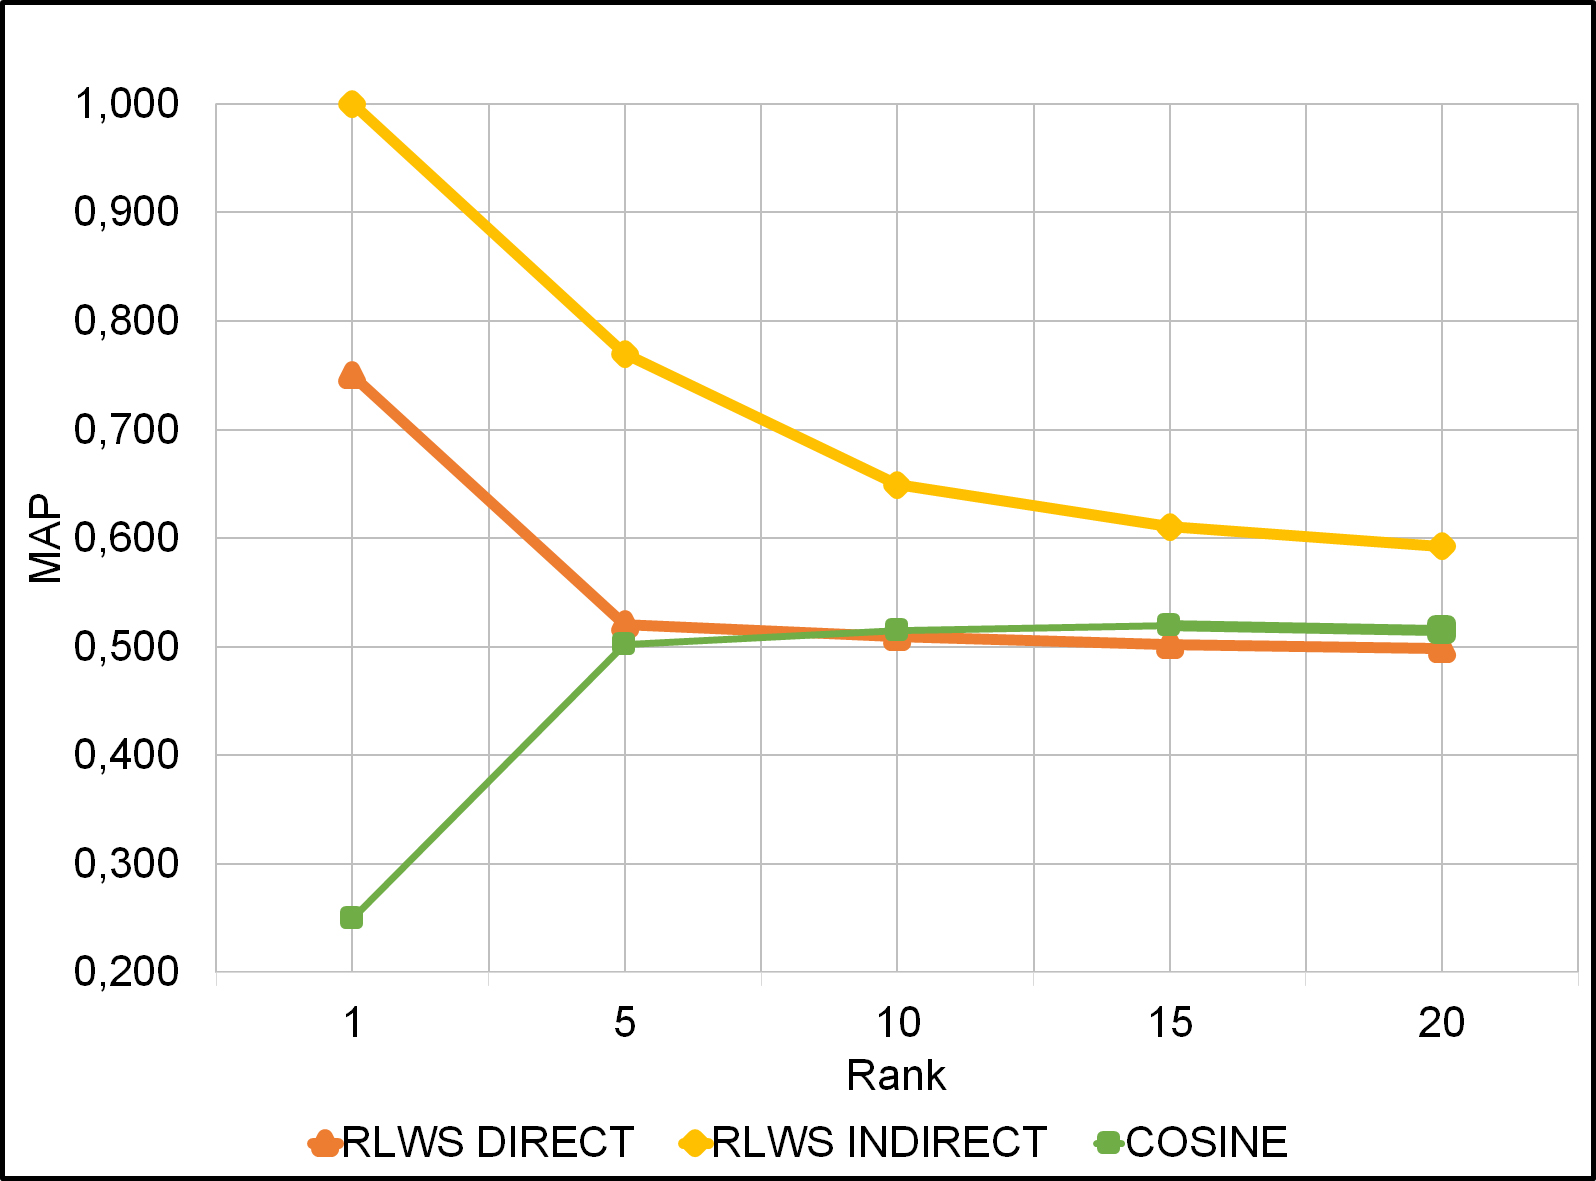
\includegraphics[width=.8\linewidth]{imagens/map_results_online.jpg}
        \caption{testes online}
        \label{fig:map_line_a}
    \end{subfigure}%
    \begin{subfigure}{.5\textwidth}
        \centering
        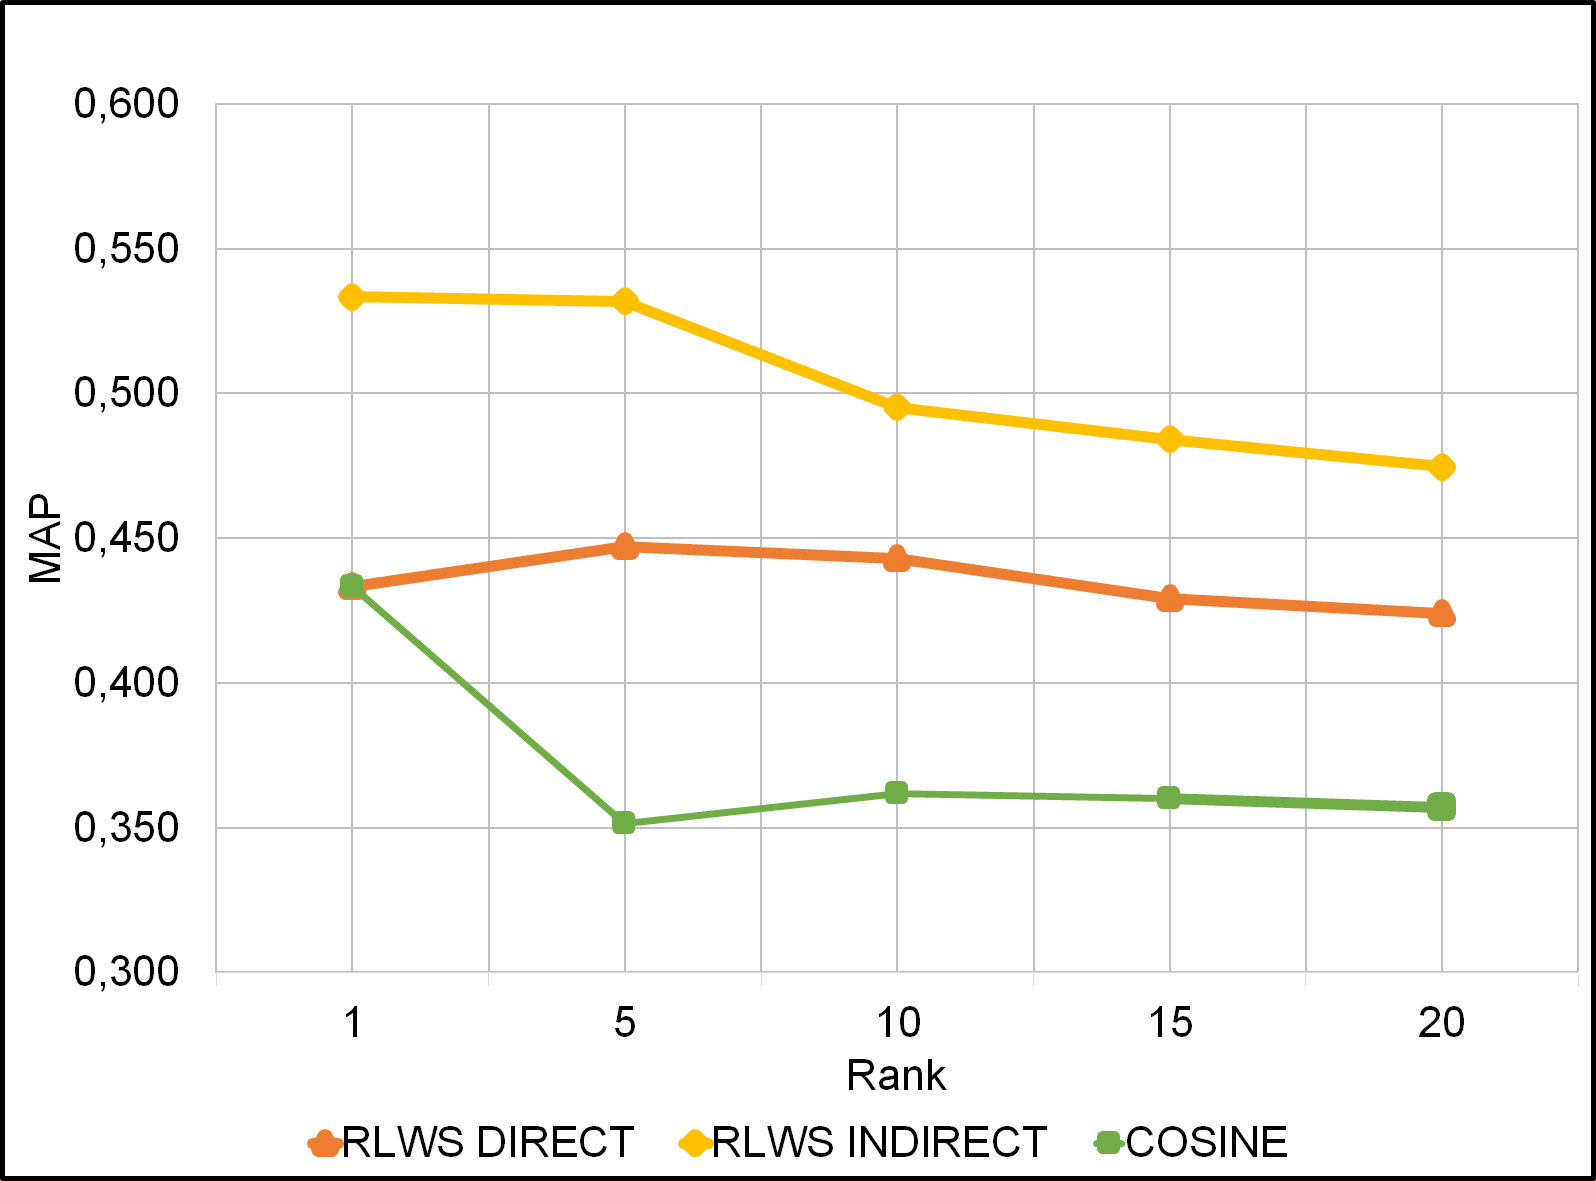
\includegraphics[width=.8\linewidth]{imagens/map_results_offline.jpg}
        \caption{testes offline}
        \label{fig:map_line_b}
    \end{subfigure}
    \caption{MAP - Gráfico com linhas dos três experimentos nos testes online e offline}
    \label{fig:map_line}
\end{figure}

\begin{figure}
    \begin{subfigure}{.5\textwidth}
        \centering
        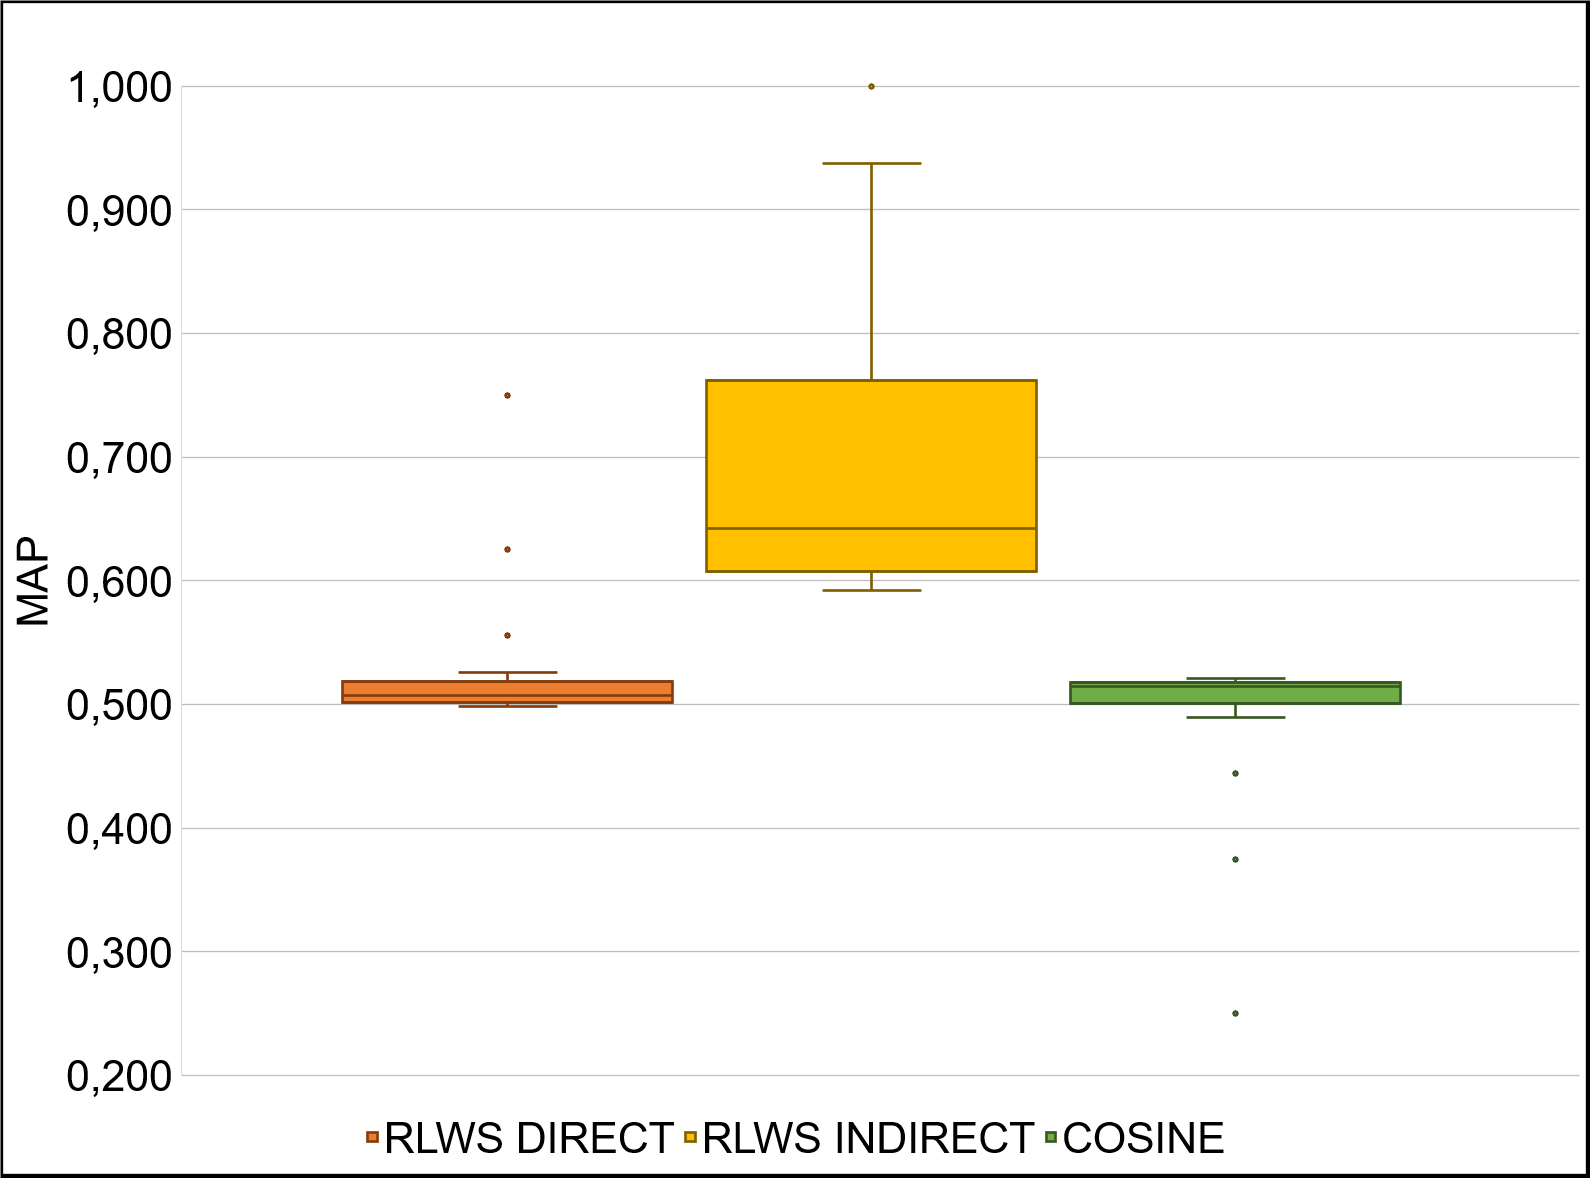
\includegraphics[width=.8\linewidth]{imagens/map_box_plot_online.jpg}
        \caption{testes online}
        \label{fig:map_box_plot_a}
    \end{subfigure}%
    \begin{subfigure}{.5\textwidth}
        \centering
        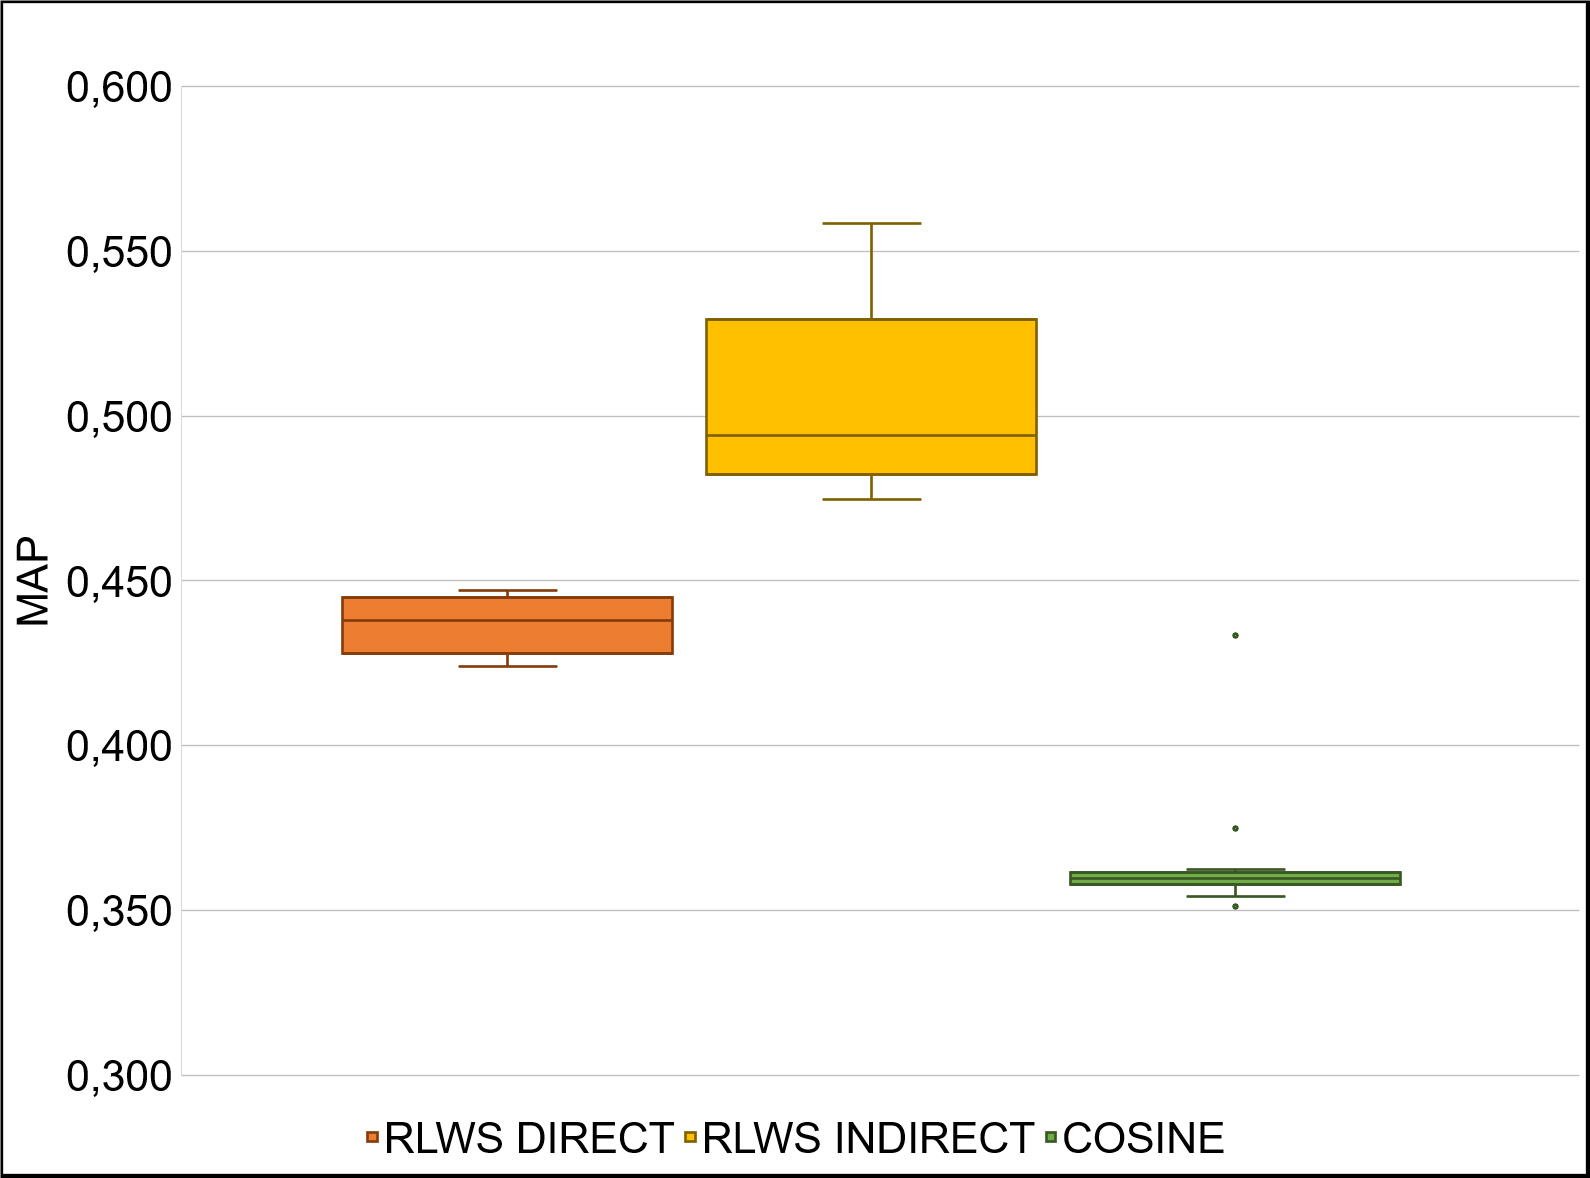
\includegraphics[width=.8\linewidth]{imagens/map_box_plot_offline.jpg}
        \caption{testes offline}
        \label{fig:map_box_plot_b}
    \end{subfigure}
    \caption{MAP - Gráfico de caixa dos três experimentos nos testes online e offline}
    \label{fig:map_box_plot}
\end{figure}

\subsection{MRR}

Para avaliar a objetividade do \ac{SR} foi utilizada a métrica \ac{MRR} perante dois conjuntos de usuários, os dos testes \textit{offline} (sendo no total de 30) e os \textit{online} (com total de 4). As Figuras \ref{fig:mrr_line} e \ref{fig:mrr_box_plot} apresentam os resultados obtidos nos três experimentos para ambos os testes. 

Assim como na métrica \ac{MAP}, também é possível observar um desempenho consideravelmente superior para o experimento 2 com a similaridade \textit{RLWS INDIRECT}, sendo 26\% (0,724 contra 0,574) superior a similaridade do cosseno nos testes \textit{offline}, para os 5 primeiros itens. Quanto ao outro par \textit{RLWS DIRECT}, obteve um resultado 11\% (0,637 contra 0,574) superior nos testes \textit{offline}. Nota-se que na Figura \ref{fig:mrr_line_a} tem-se uma linha reta com a maior nota possível, indicando que para todos os usuários nos testes online, um resultado positivo foi encontrado logo no primeiro item recomendado. Já para os testes offline é possível observar que para ambos os experimentos da métrica \ac{RLWS} foram encontrados resultados positivos já no primeiro item para mais da metade dos usuários, com o experimento \textit{COSINE} ficando um pouco abaixo. 

Os gráficos de caixa aparentes nas Figuras \ref{fig:mrr_box_plot_a} e \ref{fig:mrr_box_plot_b}, possuem em sua maioria apenas linhas retas juntamente com os \textit{outliers} devido ao fato de que a partir da 5º posição não há muito mais usuários que ainda não obtiveram uma recomendação positiva.

\begin{figure}
    \begin{subfigure}{.5\textwidth}
        \centering
        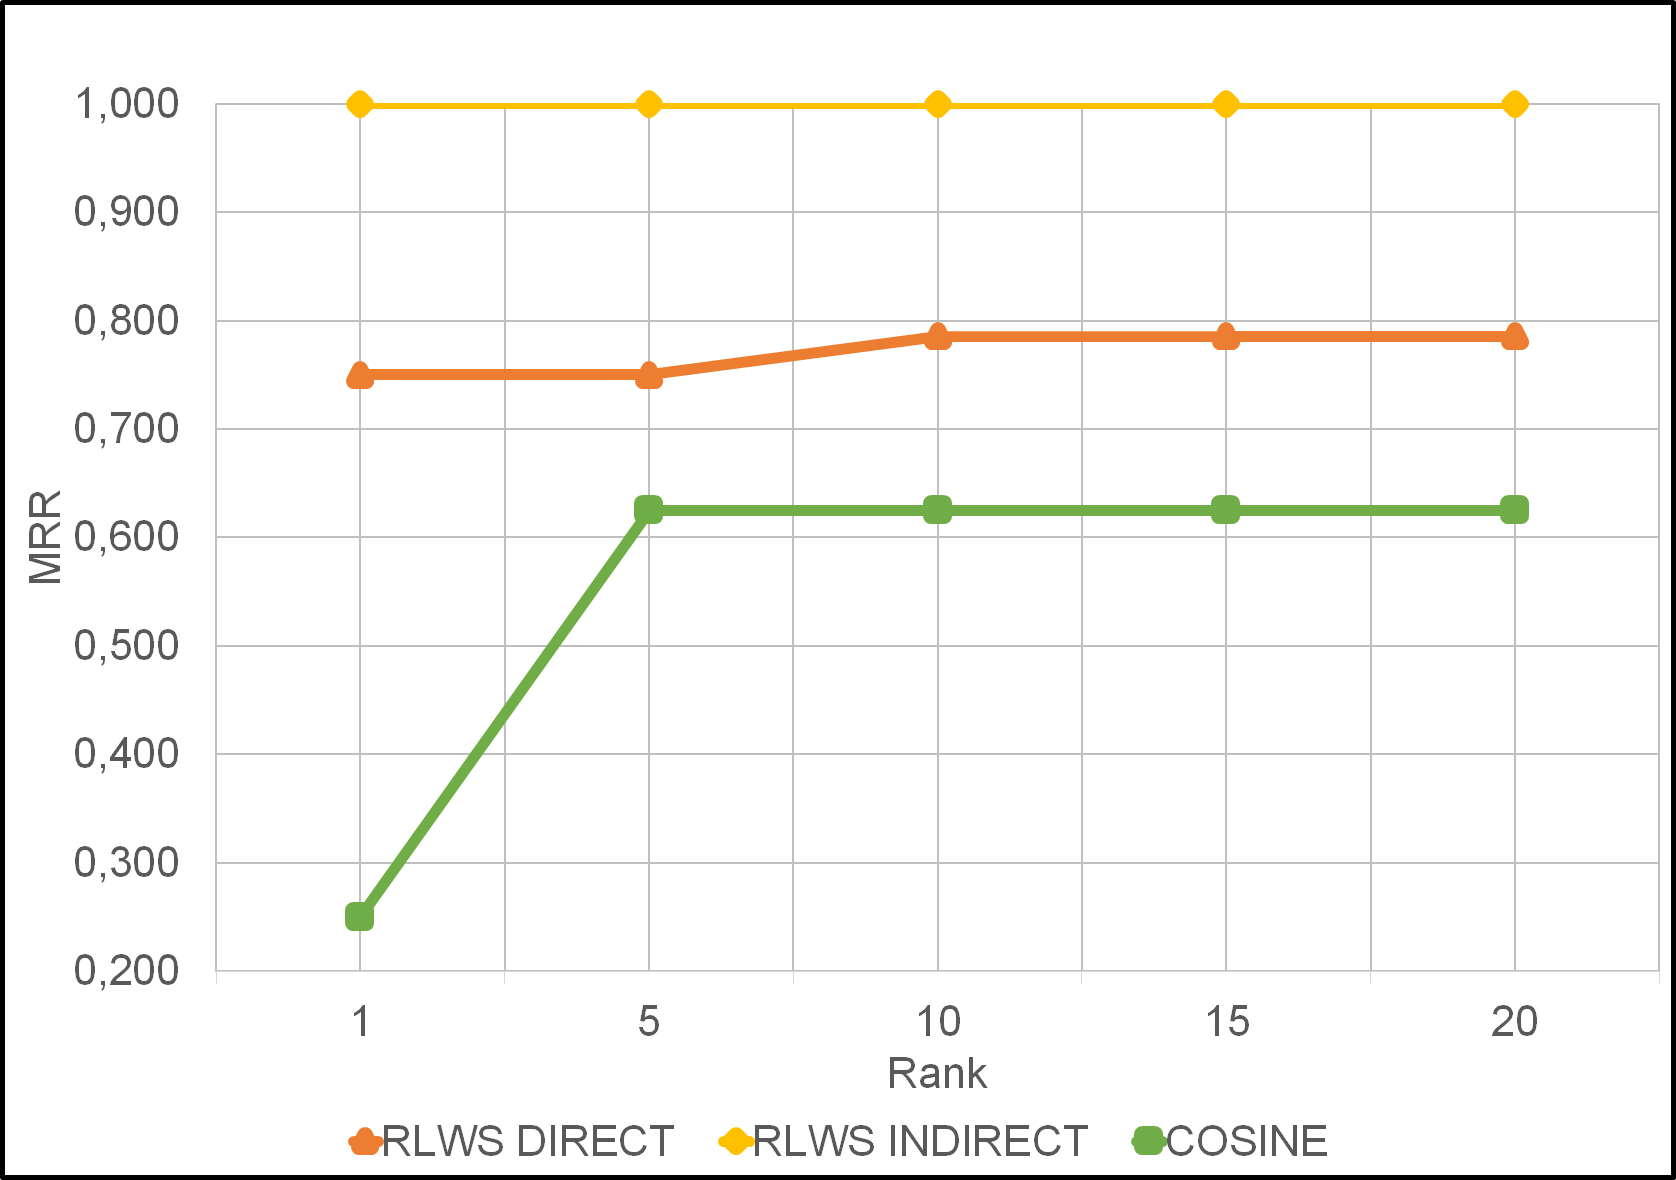
\includegraphics[width=.8\linewidth]{imagens/mrr_results_online.jpg}
        \caption{testes online}
        \label{fig:mrr_line_a}
    \end{subfigure}%
    \begin{subfigure}{.5\textwidth}
        \centering
        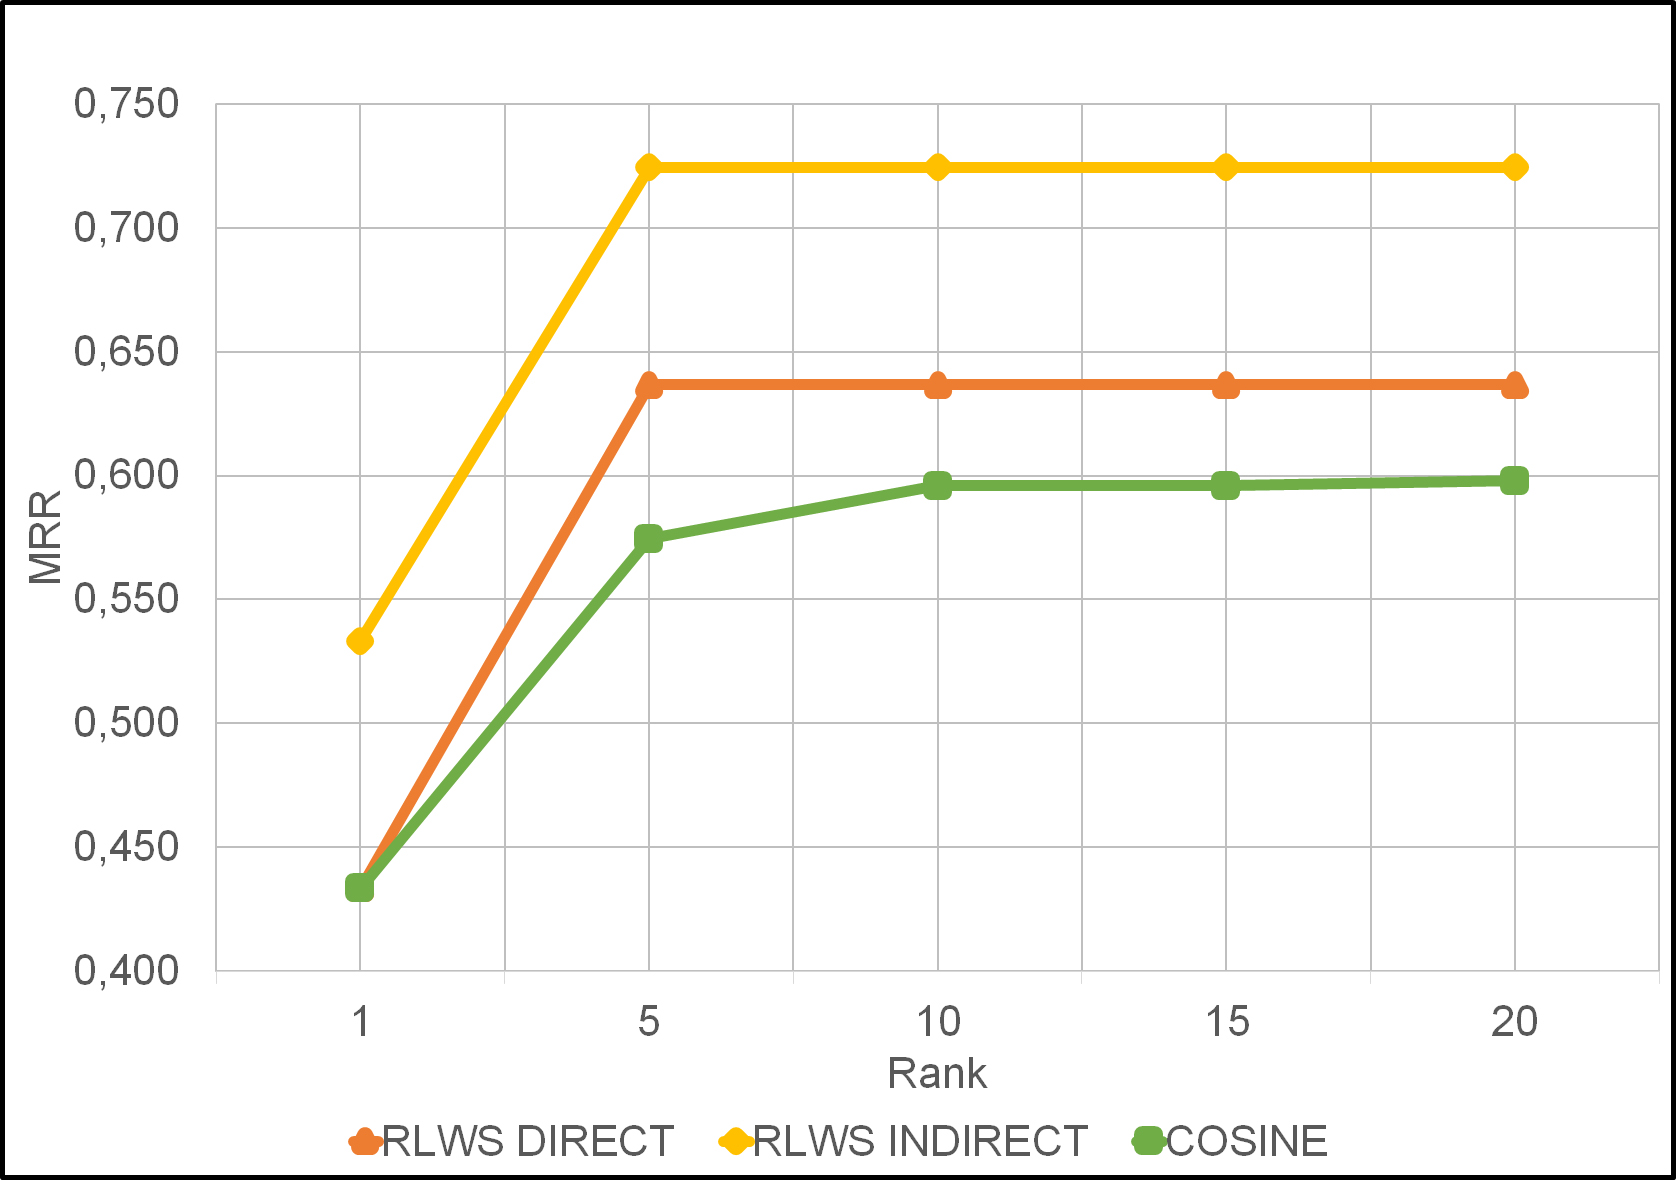
\includegraphics[width=.8\linewidth]{imagens/mrr_results_offline.jpg}
        \caption{testes offline}
        \label{fig:mrr_line_b}
    \end{subfigure}
    \caption{MRR - Gráfico com linhas dos três experimentos nos testes online e offline}
    \label{fig:mrr_line}
\end{figure}

\begin{figure}
    \begin{subfigure}{.5\textwidth}
        \centering
        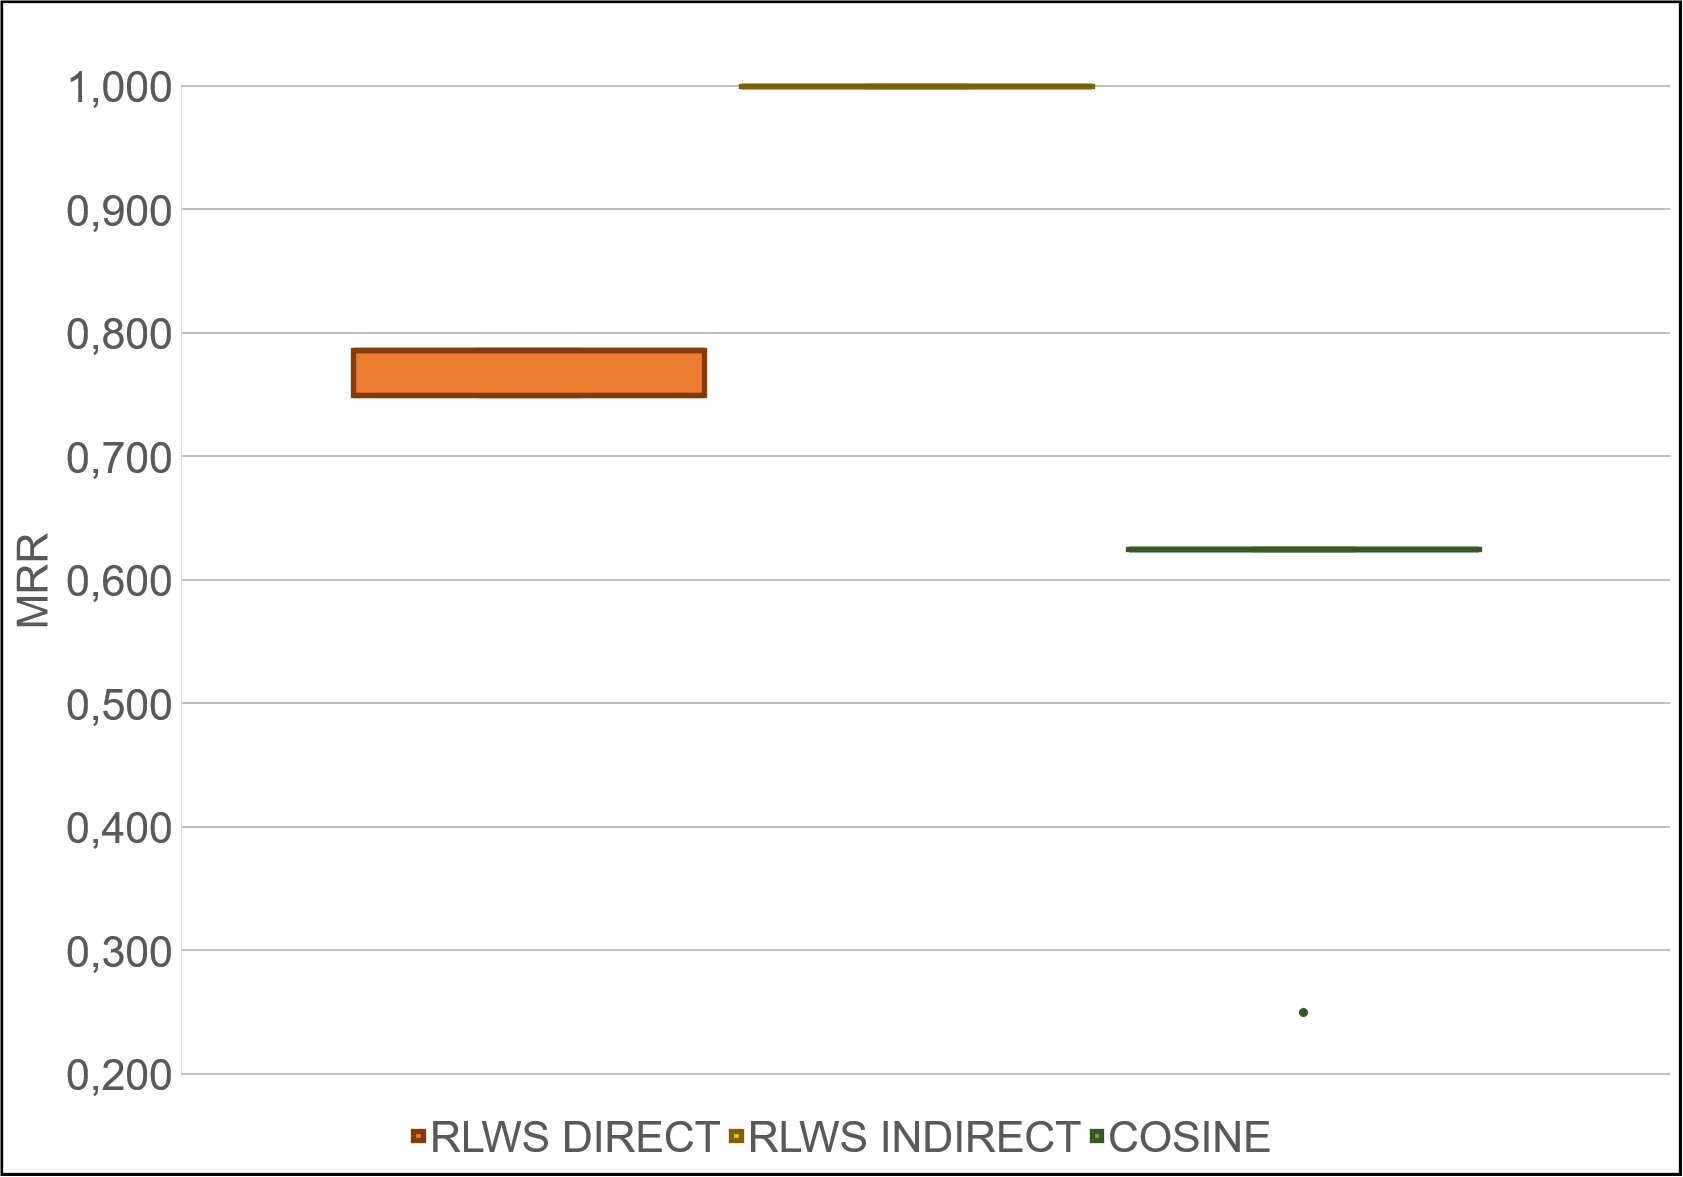
\includegraphics[width=.8\linewidth]{imagens/mrr_box_plot_online.jpg}
        \caption{testes online}
        \label{fig:mrr_box_plot_a}
    \end{subfigure}%
    \begin{subfigure}{.5\textwidth}
        \centering
        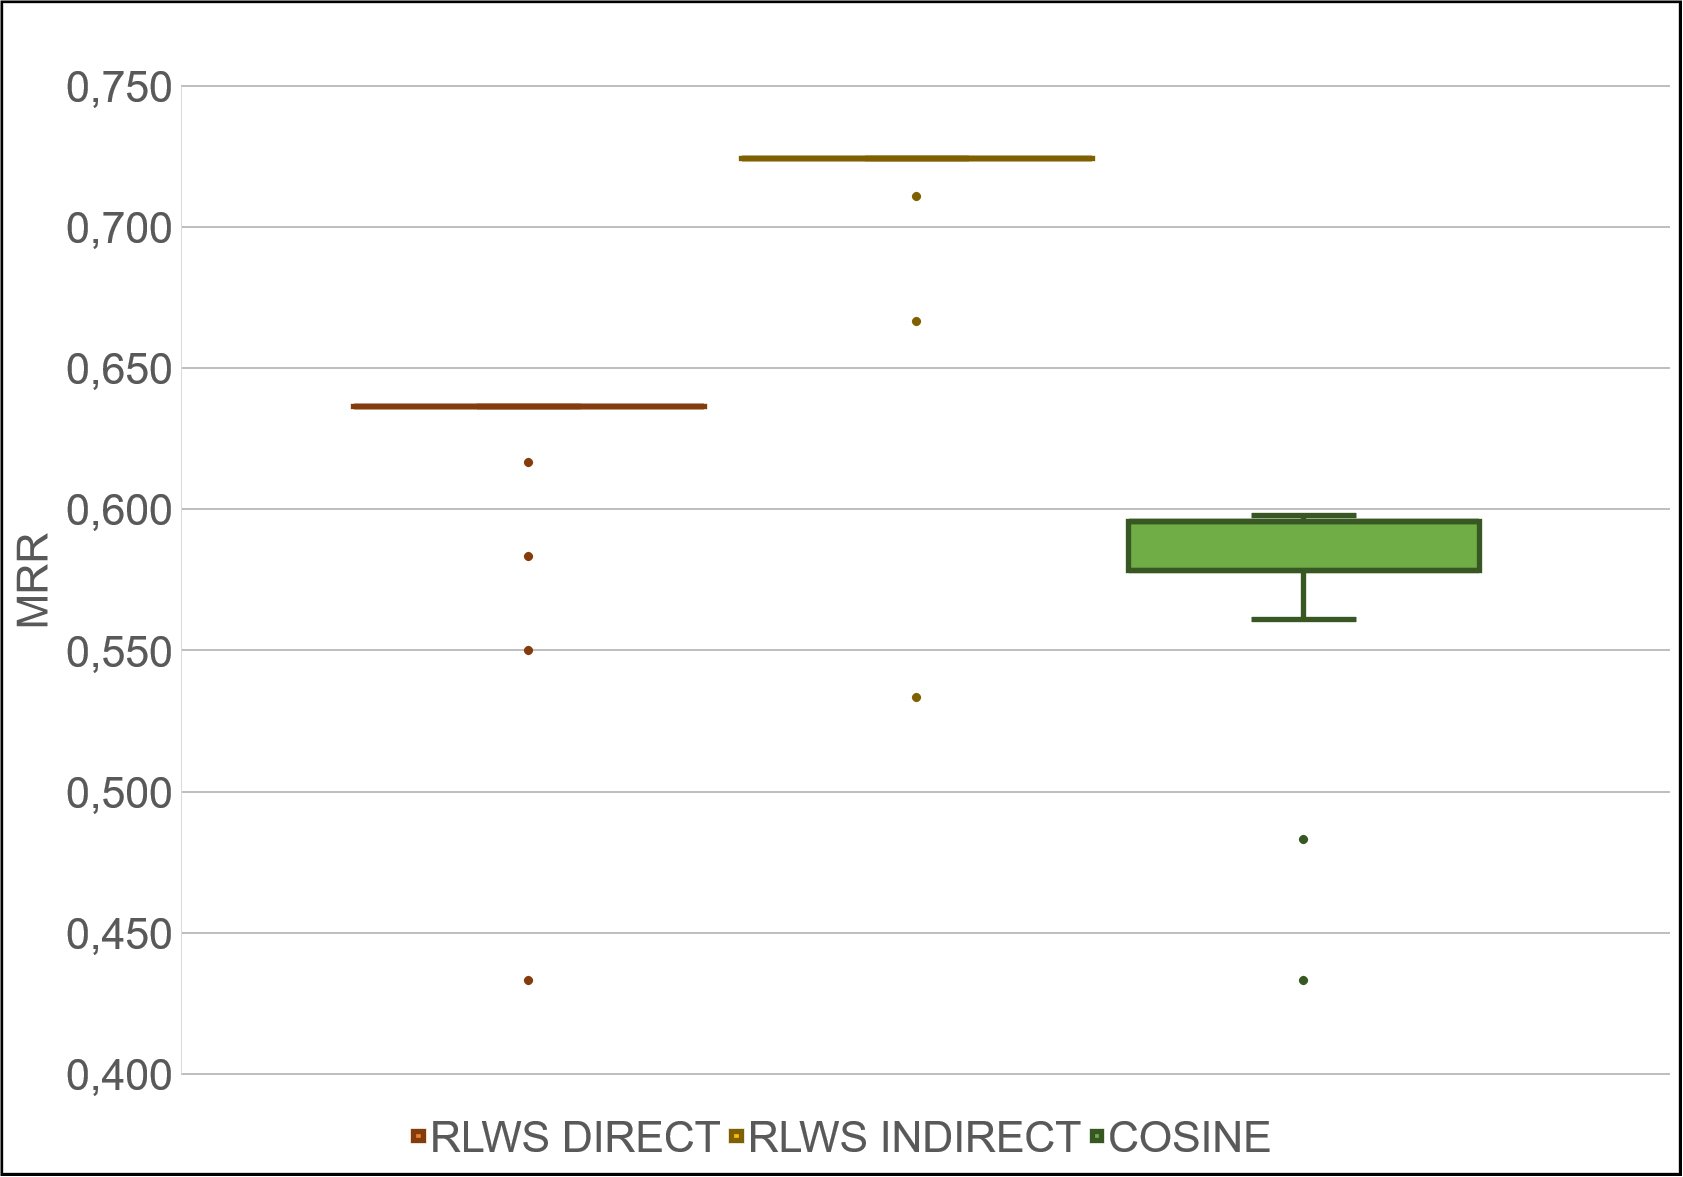
\includegraphics[width=.8\linewidth]{imagens/mrr_box_plot_offline.jpg}
        \caption{testes offline}
        \label{fig:mrr_box_plot_b}
    \end{subfigure}
    \caption{MRR - Gráfico de caixa dos três experimentos nos testes online e offline}
    \label{fig:mrr_box_plot}
\end{figure}

\section{Discussão dos resultados}

Utilizando as métricas apresentadas na metodologia foi possível observar que em especial ao uso de relacionamentos indiretos entre termos, obteve-se um resultado consideravelmente superior a métrica da similaridade do cosseno. Já quanto a variante \textbf{RLWS DIRECT}, obteve um resultado misto, sendo na maior parte das vezes superior em relação a métrica comparada. Ainda que com um grupo de testes limitado, os resultados indicam que é possível tirar proveito de uma análise semântica entre termos, podendo trazer resultados melhores de que uma análise sintática. Outra observação trata-se de que durante as entrevistas dos usuários nos testes \textit{online}, foi notado que o uso da descrição dos itens como \textit{feature} para construção do modelo de recomendação, aparentemente gerou recomendações que \enquote{fugiram à bolha tradicional} de resultados, algo que era um dos pontos do problema apresentado no capítulo \ref{cap:introducao}. Contudo, para um diversa quantidade de usuários o uso de certas \textit{features} dos itens, como ano de lançamento, gênero, autor ainda podem obter bons resultados, em especial de que é difícil avaliar se o modelo do usuário baseado na sinopse dos filmes, obtendo os termos mais relevantes, consegue captar corretamente suas preferências de narrativa, além de que o uso de outras características dos itens podem ser mais relevantes de usuário para usuário.

Outro ponto importante para ressaltar trata-se de que como o modelo de recomendação (ver seção \ref{ssec:rec_alg}) utiliza a descrição do item, um dado não estruturado, torna o sistema não muito dependente do domínio aplicado, sendo perfeitamente possível de ser utilizado numa recomendação para livros, por exemplo. Ainda que a similaridade semântica proposta seja intuitivamente coerente e de que é possível utilizá-la para modelar recomendações potencialmente mais precisas que métodos tradicionais, não seria tão adequada para comparações de textos grandes, sendo o objetivo para modelar um \ac{SR}, devido ao alto custo e carga de consultas a serem realizadas no DBPedia. Para comparar recursos individualmente ou uma coleção de palavras em pequenos textos, seria o uso mais indicado para tal similaridade.

\section{Pontos de melhorias}

Alguns desafios foram encontrados durante a construção do sistema de recomendação, principalmente relacionados a métrica de similaridade. Notou-se que a ambiguidade é um grande problema para análise de recursos na DBPedia\footnote{http://wiki.dbpedia.org}, inclusive ambiguidade em dois sentidos. O primeiro deve-se à ambiguidade no próprio serviço da web semântica que é vista pela propriedade \textit{dbo:wikiPageDisambiguates}, como no exemplo do termo \enquote{Paraná}, que pode ser resolvido para o estado brasileiro, rio ou clube de futebol. Quando uma pesquisa com termo ambíguo é realizada a contagem de links torna-se menos eficaz do que feita sabendo qual termo específico está se referindo. 

O segundo sentido de ambiguidade é a da gerada pela propriedade \textit{dbo:wikiPageRedirects}, que trata-se de como o termo é resolvido para seu nome final, comportando-se como \textit{alias}. Quando se busca um termo como \textit{Automobile}, o mesmo é redirecionado para \textit{Car} como \ac{URI} final, isso para todos os possíveis \enquote{sinônimos}. Ainda que no sistema sejam considerados termos iguais devido à análise de redirecionamentos entre si, quando se compara com outro termo, existe uma divergência para pior na contagem de links indiretos. Em futuros trabalhos poderá ser feito um ajuste nas consultas para que a contagem de links diretos e indiretos sejam mais precisas, diminuindo os problemas de ambiguidade.

Outra questão importante trata-se do custo para se executar o modelo de recomendação proposto, pois ainda que o limite superior da complexidade de tempo seja $O(|Y| * |M_u| * |D_u|)$, dentro do esperado, o modelo do usuário e de filmes tendo um custo $|M_u| * |D_u|$, na prática torna-se um conjunto de termos grande para ser executado no DBPedia. É possível identificar este problema pela Equação \ref{eq:comb_term} que demonstra o cálculo de todas as combinações de termos possíveis, sendo $n$ o total de termos associados a \ac{URI}, que apenas utilizando os 5.107 filmes, foram encontrados 18630, resultado num total de 173.529.135 comparações possíveis. Ainda que este seja o limite teórico, e de que muitos termos não venham a ser comparados, é possível notar o quanto este número pode crescer rapidamente, sendo uma alta carga de comparações, mesmo utilizando \textit{multithreading}\footnote{Multithreading trata-se da possibilidade de trabalhar com múltiplas linhas execução concorrente, tornando um processamento de dados paralelo invés de linear.} e a estrutura de \textit{cache} da contagem de links proposta na seção \ref{sec:cache}.

\begin{equation}
	C(n, 2) = \frac{n!}{2!(n - 2)!}
\label{eq:comb_term}
\end{equation}

O objetivo não é alterar o custo dado pela equação das combinações, mas verificar maneiras de diminuir os modelos para recomendação, assim reduzindo a carga teórica de consultas no DBPedia. Inclusive este problema é um dos fatores que dificultaram a execução de testes com mais usuários, algo que precisa de mais tempo para ter um conjunto maior de comparações. Com essas melhorias realizadas nos modelos, será possível expandir mais facilmente os testes \textit{online}, inclusive relacionado a este ponto também facilitaria a construção de uma plataforma online na Web para que o usuário pudesse escolher suas preferências, exibindo as recomendações para que ele mesmo avalie, dispensando o uso de entrevistas.

Um último ponto de melhoria trata-se do processo de \ac{NLP}, onde foram utilizados modelos pré-treinados oferecidos pela biblioteca \textit{OpenNLP}\footnote{https://opennlp.apache.org}. Com o uso deste modelo ocorreram diversas falhas ao reconhecer nomes de entidades (processo \ac{NER}). Para isso existem algumas possibilidades, como a de realizar um treinamento baseado nos textos dos filmes do próprio projeto, ou experimentar outras ferramentas como a \textit{Stanford CoreNLP}\footnote{https://stanfordnlp.github.io/CoreNLP/}.

\section{Sumário}

Neste capítulo foram apresentados os resultados obtidos com o sistema de recomendação construído, assim como uma análise da métrica de similaridade semântica. Para isso foram discutidas as metodologias junto com os dados utilizadas, além de estudadas as métricas que foram usadas nos resultados.


\bibliographystyle{natbib}
\addcontentsline{toc}{chapter}{\bibliographytocname}
\bibliography{references}

% Appendix
%\clearpage
%\addappheadtotoc
%\appendix
%\appendixpage
%\chapter{Formulário}
\label{ap:formulario}


\def \tick{
$[$\hspace{0.3cm}$]$
}

\def \twooption#1#2{
\tick #1.  \tick #2.
}

\def \threeoption#1#2#3{
\tick #1.\newline
\tick #2.\newline
\tick #3.
}

\def \fouroption#1#2#3#4{
\tick #1.\newline
\tick #2.\newline
\tick #3.\newline
\tick #4.
}

\def \fiveoption#1#2#3#4#5{
\tick #1.\newline
\tick #2.\newline
\tick #3.\newline
\tick #4.\newline
\tick #5.
}
\def \datefield{
%date fied used in time sheets
    /\hspace{0.4cm}/
}

\def \rcolor{
%table row color
    \rowcolor[gray]{0.9}
}

\def \hcolor{
    \rowcolor[gray]{0.7}
}


\section{Formulário para o usuário do NLP Discovery}
\label{ap:sec:feedback}

\textbf{Nome: }
\\
\line(1,0){380}
\\
\textbf{Você tem algum conhecimento técnico a respeito de Serviços Web? }
\\
\twooption{Sim}{Não}
\\
\textbf{Encontrou alguma dificuldade ao utilizar a ferramenta?}
\\
\twooption{Sim}{Não}
\\
\textbf{Caso tenha respondido "Sim", detalhe a dificuldade encontrada:}
\\
\line(1,0){410}
\\
\line(1,0){410}
\\
\line(1,0){410}
\\
\line(1,0){410}
\\
\textbf{Qual foi a consulta realizada na ferramenta (Digite exatamente o mesmo texto que digitou na caixa de pesquisa da ferramenta)?  }
\\
\line(1,0){410}
\\
\line(1,0){410}
\\
\line(1,0){410}
\\
\line(1,0){410}
\\
\textbf{A busca gerou algum resultado relevante?}
\\
\twooption{Sim}{Não}
\\
\textbf{Caso tenha respondido "Sim", qual a posição do Serviço relevante no resultado?}
\\
\line(1,0){100}
\\


\end{document}